%
% !TEX encoding = UTF-8 Unicode
% !TEX TS-program = pdflatex
% !TEX root = Tesi.tex
% !TEX spellcheck = it-IT
%
% 	PREAMBOLO
%
\documentclass[12pt,	% 10-11-12pt (12pt preferibile)
	a4paper,		%
	twoside,		% or oneside
	openright,		% new chapter in odd page
	titlepage,	 	% 
	]{book}%
%
\usepackage[T1]{fontenc}		% output
%
\usepackage[utf8]{inputenc}		% input. Also [latin1] 
%
\usepackage[english,italian]{babel}	% default italian
%
\usepackage{microtype}		% micro-tipografia
%
% 	LAYOUT - MARGINI - RILEGATURA
%
\usepackage[binding=5mm]{layaureo} 	% margins optimized for A4; 5 mm binding
%
\usepackage{emptypage}		% empty page without header and footer
%
\usepackage{indentfirst}	% indent first paragraph of every section
%
% \usepackage{booktabs}		% tables (\toprule, \midrule, \bottomrule). Uncomment if necessary
%
% \usepackage{tabularx}		% Uncomment if necessary
%
\usepackage{graphicx}		% image
%
\usepackage[figuresright]{rotating}	% tables at 90°
%
% \usepackage{subfig}			% subfigures, subtables. Uncomment if necessary
%
\usepackage{caption}		% captions
%
\usepackage{listings}		% piece of code
%
\usepackage[font=small]{quoting}	% citation
%
% \usepackage{amsmath,amssymb}	% math
%
% \usepackage{mathtools}		% math
%
% \usepackage{amsthm}		% math
%
\usepackage[output-decimal-marker={,}]{siunitx}	
%
\usepackage[italian]{varioref}	
%
\usepackage{relsize}			% make text larger or smaller than the surrounding text
%
\usepackage{csquotes} %italian=guillemets
%
\usepackage{hyperref}
%
\usepackage[style=ieee,	
	sorting = none,		% reorder bib entries
	backref,			% back ref citations
	natbib=true, 		% compatibility with natbib
	hyperref,
	backend=bibtex,		% bib engine
	defernumbers=true,	% citation order inside text
	]{biblatex}%
%
\bibliography{Bibliografia}
%
\usepackage[dvipsnames]{xcolor}	% colori - 68 colori predefiniti:
% 				% http://en.wikibooks.org/wiki/LaTeX/Colors
%
\usepackage{lipsum}			% lorem ipsum
%
\usepackage{eurosym}		% Euro symbol
%
\usepackage{hyperref}		% 
%
\usepackage{bookmark}		% 
%
\usepackage{guit}			% Guit symbol
%
\usepackage{fancyhdr}		% custom header and footer
%
\setlength{\headheight}{15pt}
%
\usepackage{colortbl}		% per colorare i filetti delle tabelle
%
\usepackage[footnote,		% descrizione acronimo fatta a piè di pagina
	smaller,			% acronimo scritto con dimensione ridotta
	]{acronym}		% acronimi
%
% \usepackage{multirow}		% celle tabelle alte più di una riga
%
\usepackage{pdfpages}		% inclusione di files pdf esterni
%
\usepackage{setspace}		% imposto l'interlinea del documento
%
\linespread{1.2}
%
\usepackage[nottoc,numbib]{tocbibind}	
%
\usepackage{gensymb}
%
\usepackage{float}
%
\usepackage[xindy,toc,nonumberlist]{glossaries}	% includo il glossario
%
\makeglossaries
%
%
% !TEX encoding = UTF-8 Unicode
% !TEX TS-program = pdflatex
% !TEX root = Tesi.tex
% !TEX spellcheck = it-IT
%
% \addcontentsline{toc}{chapter}{Glossario}
%
\newglossaryentry{dematerializzazione}
{
	name=Dematerializzazione,
	description={Processo di innovazione tecnologica che prevede la conversione di qualunque documento cartaceo in un adeguato formato digitale, fruibile con mezzi informatici, finalizzata alla distruzione della materialità. Il risultato è una stringa digitale che soddisfa i requisiti tecnici e legali previsti per ciascun tipo di documento elettronico nominato (per esempio, la "ricetta elettronica") o, in termini più estesi, le convenzioni stabilite dalla comunità nella quale il documento assume pieno valore.}
}
%%%%
\newglossaryentry{EHR-SF}
{
	name=EHR-S,
	description={L’Electronic Health Record – System Functional Model è uno degli standard realizzati da HL7 International ed è approvato, inoltre, da ISO come ISO/HL7 10781. Il modello
	comprende 322 funzioni e 2.310 criteri di conformità formali.}
}
%%%%
\newglossaryentry{ricetta bianca}
{
	name=Ricetta bianca,
	description={ricetta che il medico compila su carta bianca, sulla quale siano però riportati: il nome e cognome del medico; la data; il luogo; la firma autografa del medico. In questo caso, il nome dell’assistito non è strettamente necessario. Su ricetta bianca possono essere prescritte tutte le prestazioni di specialistica ambulatoriale, di diagnostica strumentale e di laboratorio, di norma correlate alla propria branca di specializzazione e i farmaci, prestazioni che saranno sempre a carico del cittadino assistito. Per la prescrizione a carico del servizio sanitario è infatti necessaria la ricetta del ricettario regionale ed è valida in tutte le farmacie italiane.}
}
%%%
\newglossaryentry{ricetta rossa}
{
	name=Ricetta rossa,
	description={ricetta che può essere compilata solamente dai medici dipendenti di strutture pubbliche o convenzionati con il servizio sanitario nazionale e viene utilizzata per la prescrizione di una terapia farmacologica, la prescrizione di un esame diagnostico o una visita specialistica a carico del servizio sanitario. L’uso di una ricetta rossa non permette l’erogazione a carico del servizio sanitario di farmaci o prodotti parafarmaceutici non compresi tra le formulazioni del prontuario farmaceutico regionale, né di esami, visite o terapie non comprese nei Lea o nelle disposizioni della propria regione.}
}
%%%%
\newglossaryentry{asimmetrica}
{
	name={Cifratura asimmetrica},
	description={tecnica di cifratura in cui chiave di crittazione e chiave di decrittazione sono diverse ma complementari, ossia un messaggio cifrato con la prima pu` o essere decifrato con la seconda e viceversa; in questo caso ogni utente possiede una coppia di chiavi, una pubblica (nota a tutti) ed una privata (nota solo a se stesso) e per questo, dati N utenti, l’insieme complessivo di chiavi è numericamente pari a \emph{2xN}. È una tecnica di cifratura più sicura rispetto a quella simmetrica, ma allo stesso tempo computazionalmente più complessa}
}
%%%%%
\newglossaryentry{simmetrica}
{
	name={Cifratura simmetrica},
	description={tecnica di cifratura tale per cui chiave di crittazione e chiave di decrittazione coincidono, rendendo l’algoritmo molto performante e semplice da implementare; in questo scenario, ogni chiave identifica una coppia di utenti e per questo, dati N utenti, l’insieme complessivo di chiavi definite ha cardinalità: $\binom{N}{2}$}
}
%%%%
\newglossaryentry{dos}
{
	name={Attacco DoS},
	description={attacco informatico che mira a saturare una o più risorse di rete (inviandogli numerose richieste) con lo scopo, solitamente, di rendere un server incapace di erogare servizi ai propri clienti. Se la richiesta proviene da diversi siti contemporaneamente, si parla di \emph{Attacco DDoS} (Distributed Denial of Service)}
}
%%%%%
\newglossaryentry{hash}
{
	name={Hash crittografico},
	description={algoritmo matematico che mappa dei dati di lunghezza arbitraria (messaggio) in una stringa binaria di dimensione fissa chiamata valore di hash, ma spesso viene indicata anche con il termine inglese message digest (o semplicemente digest). Tale funzione di hash è progettata per essere unidirezionale (one-way), ovvero una funzione difficile da invertire: l'unico modo per ricreare i dati di input dall'output di una funzione di hash ideale è quello di tentare una ricerca di forza-bruta di possibili input per vedere se vi è corrispondenza (match). In alternativa, si potrebbe utilizzare una tabella arcobaleno di hash corrispondenti. La funzione di hash deve avere alcune proprietà fondamentali:
		\begin{itemize}
			\item il calcolo dell'hash deve essere semplice indipendentemente dal dato di partenza.
			\item deve essere difficile se non impossibile risalire al dato originario dall'hash.
			\item deve essere improbabile che due messaggi differenti abbiano lo stesso hash
		\end{itemize} 
	}
}
%
\newglossaryentry{pgp}
{
	name={Pretty Good Privacy (PGP)},
	description={è una famiglia di software di crittografia per autenticazione e privacy, da cui è derivato lo standard OpenPGP. È probabilmente il crittosistema più adottato al mondo, descritto dal crittografo Bruce Schneier come il modo per arrivare "probabilmente il più vicino alla crittografia di livello militare". Caratteristica principale: robusto ad attacchi MITM (man in the middle). Per esempio con il metodo forza bruta l’attaccante necessiterebbe di un calcolatore con immense capacità di calcolo e di tempi di elaborazioni “universali” (ammesso che il dispositivo che conserva messaggio e chiave privata del mittente non sia compromesso). Funzionamento: il mittente usa la chiave pubblica (cifratura asimmetrica) del destinatario per cifrare una chiave comune (cifratura simmetrica) con cui si cifra il testo in chiaro del messaggio}
}
%%%%%
\newglossaryentry{qrcode}
{
	name={Qr-code},
	description={Un codice QR (abbreviazione di Quick Response Code) è un codice a barre bidimensionale (o codice 2D), composto da moduli neri disposti all'interno di uno schema di forma quadrata. Viene impiegato per memorizzare informazioni generalmente destinate a essere lette tramite un telefono cellulare o uno smartphone. In un solo crittogramma possono essere contenuti fino a 7.089 caratteri numerici o 4.296 alfanumerici. Genericamente il formato matriciale è di 29x29 quadratini e contiene 48 alfanumerici. Il codice è stato sviluppato al fine di permettere una rapida decodifica del suo contenuto}
}%%%%
\newglossaryentry{permissioned}
{
	name={Permissioned Ledger},
	description={Un sistema \emph{permissioned} è quello in cui l'identità per gli utenti è autorizzata nella whitelist (o nella black list); è il metodo comune di gestione dell'identità nella finanza tradizionale. Al contrario, un sistema privo di autorizzazioni è quello in cui l'identità dei partecipanti è caratterizzata da pseudonimi o addirittura anonima. Bitcoin è stato originariamente progettato con parametri privi di permessi.}
}%%%%

%
\glstoctrue
%
%
% !TEX encoding = UTF-8 Unicode
% !TEX TS-program = pdflatex
% !TEX root = Tesi.tex
% !TEX spellcheck = it-IT
%
% ------------------------------------------------------------------------ %
% Other personal commands
% ------------------------------------------------------------------------ %
%
\newcommand{\myName}{Claudio Petrocco}			% autore
\newcommand{\myMatricola}{1065591}			% matricola
\newcommand{\myTitle}{Gestione delle prescrizioni mediche dematerializzate utilizzando una Blockchain privata}	% titolo
\newcommand{\myUni}{Università Politecnica delle Marche}		% università
\newcommand{\myDegree}{Ingegneria Informatica e dell'Automazione}		% laurea
\newcommand{\myThesis}{Tesi di Laurea Magistrale}	% tipo di tesi
\newcommand{\myDepartment}{Dipartimento dell'Informazione}	% dipartimento
\newcommand{\myProf}{Prof.~Luca~Spalazzi}		% relatore
\newcommand{\myOtherProf}{Ing.~Marco~Baldi}		% eventuale correlatore
\newcommand{\myLocation}{Ancona}			% dove
\newcommand{\myTime}{Dicembre 2017}			% quando
\newcommand{\myAcademicYear}{2016--2017}		% anno accademico
%
% ------------------------------------------------------------------------ %
% Amsmath, amssymb, amsthm
% ------------------------------------------------------------------------ %
%
% Uncomment if necessary
%
% \newenvironment{sistema}%
% {\left\lbrace\begin{array}{@{}l@{}}}%
% {\end{array}\right.}
% %
% % epsilon theta rho phi
% \renewcommand{\epsilon}{\varepsilon}
% \renewcommand{\theta}{\vartheta}
% %\renewcommand{\rho}{\varrho}
% \renewcommand{\phi}{\varphi}
% %
% \renewcommand{\vec}{\mathbf} 
%
% ------------------------------------------------------------------------ %
% Xcolor
% ------------------------------------------------------------------------ %
%
% webcolors
\definecolor{webgreen}{rgb}{0,.5,0}
\definecolor{webbrown}{rgb}{.6,0,0}
%
% Blue
\definecolor{darkbluePoliMi}{rgb}{0,0.18,0.40}	%rgb(0, 46, 103)
\definecolor{midbluePoliMi}{rgb}{0.33,0.47,0.62}	%rgb(84, 121, 157)
\definecolor{lightbluePoliMi}{rgb}{0.53,0.64,0.73}	%rgb(134, 163, 186)
\definecolor{orangePoliMi}{rgb}{1,0.59,0}		%rgb(255, 151, 0)
%
%
% ------------------------------------------------------------------------ %
% Listings
% ------------------------------------------------------------------------ %
%
\lstset{
	basicstyle=\smaller[0]\ttfamily,		% Black & White:
	keywordstyle=\color{RoyalBlue},	% keywordstyle=\color{black}\bfseries,
	commentstyle=\color{webgreen},	% commentstyle=\color{gray},
	stringstyle=\color{webbrown},		% stringstyle=\color{black},
	numbers=left,
	numberstyle=\smaller[2],
	stepnumber=1,
	numbersep=8pt,
	showspaces=false,
	showstringspaces=false,
	showtabs=false,
	breaklines=true,
	frameround=ffff,
	frame=single,
	tabsize=2,
	captionpos=t,
	breakatwhitespace=false,
}
%
% Solution to the encoding issue
\lstset{literate=
	{á}{{\'a}}1 {é}{{\'e}}1 {í}{{\'i}}1 {ó}{{\'o}}1 {ú}{{\'u}}1
	{Á}{{\'A}}1 {É}{{\'E}}1 {Í}{{\'I}}1 {Ó}{{\'O}}1 {Ú}{{\'U}}1
	{à}{{\`a}}1 {è}{{\`e}}1 {ì}{{\`i}}1 {ò}{{\`o}}1 {ù}{{\`u}}1
	{À}{{\`A}}1 {È}{{\'E}}1 {Ì}{{\`I}}1 {Ò}{{\`O}}1 {Ù}{{\`U}}1
	{ä}{{\"a}}1 {ë}{{\"e}}1 {ï}{{\"i}}1 {ö}{{\"o}}1 {ü}{{\"u}}1
	{Ä}{{\"A}}1 {Ë}{{\"E}}1 {Ï}{{\"I}}1 {Ö}{{\"O}}1 {Ü}{{\"U}}1
	{â}{{\^a}}1 {ê}{{\^e}}1 {î}{{\^i}}1 {ô}{{\^o}}1 {û}{{\^u}}1
	{Â}{{\^A}}1 {Ê}{{\^E}}1 {Î}{{\^I}}1 {Ô}{{\^O}}1 {Û}{{\^U}}1
	{œ}{{\oe}}1 {Œ}{{\OE}}1 {æ}{{\ae}}1 {Æ}{{\AE}}1 {ß}{{\ss}}1
	{ç}{{\c c}}1 {Ç}{{\c C}}1 {ø}{{\o}}1 {å}{{\r a}}1 {Å}{{\r A}}1
	{€}{{\EUR}}1 {£}{{\pounds}}1
}
%
% Definizione ambienti per i vari linguaggi
%
\lstnewenvironment{Matlab}{\lstset{language=Matlab}}{}
%
\lstnewenvironment{C++}{\lstset{language=C++}}{}
%
\lstnewenvironment{bash}{\lstset{language=bash}}{}
%
%
% Code listings
%
\addto\captionsitalian{\renewcommand{\lstlistingname}{Codice}}
%
\addto\captionsitalian{\renewcommand{\lstlistlistingname}{Elenco dei codici}}
%
% ------------------------------------------------------------------------ %
% Hyperref
% ------------------------------------------------------------------------ %
%
\hypersetup{
	colorlinks=true,
	linktocpage=true,
	pdfstartpage=1,
	pdfstartview=FitV,
	breaklinks=true,
	pageanchor=true,
	pdfpagemode=UseOutlines,
	bookmarksopenlevel=1,
	hypertexnames=true,
	pdfhighlight=/O,
	urlcolor=webbrown,		
	linkcolor=RoyalBlue,
	citecolor=webgreen,
	pdftitle={\myTitle},		
	pdfauthor={\textcopyright\ \myName, \myUni},
	pdfsubject={},
	pdfcreator={pdfLaTeX},
	pdfproducer={LaTeX with hyperref}
}
%
% ------------------------------------------------------------------------ %
% Graphicx
% ------------------------------------------------------------------------ %
%
\graphicspath{
	{Immagini/}
	{Immagini/Introduzione/}
	{Immagini/Sanitadigitale/}
	{Immagini/Blockchain/}
	{Immagini/Ethereum/}
	{Immagini/Quorum/}
	{Immagini/StrumentiSviluppo/}
	{Immagini/Implementazione/}
}
%
% ------------------------------------------------------------------------ %
% Fancyhdr
% ------------------------------------------------------------------------ %
%
\pagestyle{fancy}			% instead of \pagestyle{header} standard
%
\makeatletter 
%
\renewcommand{\chaptermark}[1]{	% chapter def
	\markboth{\@chapapp\ \thechapter.\ #1}{}} % Chapter / appendix
\makeatother
%
\renewcommand{\sectionmark}[1]{	% section ndef
	\markright{\thesection.\ #1}}
%
\fancyhf{}				% Empty header and footer
%
\fancyhead[LE,RO]{\bfseries}	% numero pagine in alto
%
\fancyhead[LO]{\bfseries\rightmark}	% info section in odd page
%
\fancyhead[RE]{\bfseries\leftmark}	% info chapter in even page
%
\cfoot{\thepage}
%
\renewcommand{\headrulewidth}{0.4pt}	% 
%
\renewcommand{\footrulewidth}{0pt}	% (0pt=hidden)
%
\fancypagestyle{plain}{				% begin chapter style
	\fancyhead{}			% empty header
	\fancyfoot[C]{\bfseries\thepage}		% bold numbers centered
	\renewcommand{\headrulewidth}{0pt}	% no line
}
%
% ------------------------------------------------------------------------ %
% Other
% ------------------------------------------------------------------------ %
%
% Gradiente
\newcommand{\gradiente}[1]{$\nabla #1$}
%
% puntini di omissione [...]
\newcommand{\omissis}{[\dots\negthinspace]}
%
% Eccezioni all'algoritmo di sillabazione
\hyphenation{OpenFOAM}
\hyphenation{Matlab}
\hyphenation{bash}
%
% ------------------------------------------------------------------------ %
% Finezze tipografiche per il Politecnico di Milano
% ------------------------------------------------------------------------ %
%
% Le seguenti modifiche possono essere commentate
% o adeguate ad un'altra università (es. 'Yale Blue'
% per l'università di Yale, 'Rosso Sapienza' per La Sapienza..)
%
% Filetti tabelle colorati
% \arrayrulecolor{darkbluePoliMi}
%
%
% Righe delle note a piè di pagina colorate
\renewcommand{\footnoterule}{%
	\kern -3pt
	{\color{darkbluePoliMi} \hrule width 0.4\textwidth}
	\kern 2.6pt
}
%
% ------------------------------------------------------------------------ %
% Comandi aggiuntivi inseriti 
% ------------------------------------------------------------------------ %
\renewcommand*\thesection{\arabic{section}}		% i numeri delle sezioni passano da #chapter.#section a solo #section
%
\colorlet{punct}{red!60!black}
\definecolor{background}{HTML}{EEEEEE}
\definecolor{delim}{RGB}{20,105,176}
\colorlet{numb}{magenta!60!black}
%
%define json
\lstdefinelanguage{json}{
	basicstyle=\normalfont\ttfamily\linespread{0.9}\small,
	numbers=left,
	numberstyle=\scriptsize,
	stepnumber=1,
	numbersep=7pt,
	showstringspaces=false,
	breaklines=true,
	frame=lines,
	%backgroundcolor=\color{background},
	literate=
	*{0}{{{\color{numb}0}}}{1}
	{1}{{{\color{numb}1}}}{1}
	{2}{{{\color{numb}2}}}{1}
	{3}{{{\color{numb}3}}}{1}
	{4}{{{\color{numb}4}}}{1}
	{5}{{{\color{numb}5}}}{1}
	{6}{{{\color{numb}6}}}{1}
	{7}{{{\color{numb}7}}}{1}
	{8}{{{\color{numb}8}}}{1}
	{9}{{{\color{numb}9}}}{1}
	{:}{{{\color{punct}{:}}}}{1}
	{,}{{{\color{punct}{,}}}}{1}
	{\{}{{{\color{delim}{\{}}}}{1}
	{\}}{{{\color{delim}{\}}}}}{1}
	{[}{{{\color{delim}{[}}}}{1}
	{]}{{{\color{delim}{]}}}}{1},
}%
%define javascript
\definecolor{darkgray}{rgb}{.4,.4,.4}
\definecolor{purple}{rgb}{0.65, 0.12, 0.82}
\lstdefinelanguage{JavaScript}{
	keywords={typeof, new, true, false, catch, function, return, null, catch, switch, var, if, in, while, do, else, case, break},
	keywordstyle=\color{blue}\bfseries,
	ndkeywords={class, export, boolean, throw, implements, import, this},
	ndkeywordstyle=\color{darkgray}\bfseries,
	identifierstyle=\color{black},
	frame=lines,
	basicstyle=\linespread{0.9}\small,
	sensitive=false,
	comment=[l]{//},
	morecomment=[s]{/*}{*/},
	commentstyle=\color{purple}\ttfamily,
	stringstyle=\color{red}\ttfamily,
	morestring=[b]',
	morestring=[b]"
}%
%%%%
\newenvironment{para}[1]
{%here comes what is processed before
	\noindent\textbf{#1}\hspace{1em}\ignorespaces}
{%and here what is processed after
	\par}
%%%%
% COMMAND: \pic
% SYNTAX:  \pic{PATH}!LABEL![SIZE]
% EFFECT:  Draws PATH image scaled to SIZE*columnwidth, eventually with LABEL.
% \DeclareDocumentCommand{\pic}{ m d!! O{0.5} }
% {
% 	\begin{center}\includegraphics[width=#3\columnwidth]{#1}
% 		\IfValueT{#2}
% 		{
% 			\label{#2}
% 		}
% 	\end{center}
% }
		% file con altre impostazioni
%
% ------------------------------------------------------------------------ %
% 	BEGIN DOCUMENT
% ------------------------------------------------------------------------ %
%
\begin{document}
%
% ------------------------------------------------------------------------ %
% 	FRONTMATTER
% ------------------------------------------------------------------------ %
%
\frontmatter
%

\includepdf{AltroMateriale/frontespizio.pdf}
%
%
% !TEX encoding = UTF-8 Unicode
% !TEX TS-program = pdflatex
% !TEX root = ../Tesi.tex
% !TEX spellcheck = it-IT
%
\cleardoublepage
%
% Index
%
\pdfbookmark{\contentsname}{tableofcontents}
%
\setcounter{tocdepth}{2}
%
\tableofcontents
%
\cleardoublepage
%
% figures
%
\phantomsection
%
\listoffigures
%
\cleardoublepage
%
% code listings
%
\phantomsection
%
\pdfbookmark{\lstlistlistingname}{lol}
%
\lstlistoflistings
%
\cleardoublepage
%

%
\cleardoublepage
%
% ------------------------------------------------------------------------ %
% 	MAINMATTER
% ------------------------------------------------------------------------ %
%
\mainmatter
%
% ------------------------------------------------------------------------ %
% !TEX encoding = UTF-8 Unicode
% !TEX TS-program = pdflatex
% !TEX root = ../Tesi.tex
% !TEX spellcheck = it-IT
% ------------------------------------------------------------------------ %
%
% ------------------------------------------------------------------------ %
% 	INTRODUZIONE
% ------------------------------------------------------------------------ %
%
\cleardoublepage
%
\phantomsection
%
\chapter{Introduzione}
%
\markboth{Introduzione}{Introduzione}	% headings
%
\label{cap:introduzione}
%
In poco meno di vent'anni si è passati dal floppy disk al cd e, da questo, alla chiave usb e ad altri tipi di supporti portatili di memoria, fino ad arrivare al cloud computing, eliminando di fatto la necessità del supporto fisico per produrre e preservare i dati, le informazioni e i documenti digitali. L'affermarsi continua di nuove tecnologie ha quindi modificato la concezione del \emph{documento}, in particolar modo della sua creazione e conservazione. \\	
Se fino agli anni ’90 si aveva  una visione più ristretta e univoca del document management, che sostanzialmente coincideva con la digitalizzazione di immagini e l’archiviazione ottica di documenti nati originariamente su supporti analogici (prevalentemente cartacei), negli anni 2000 si è passati al concetto già più complesso di \emph{Gestione documentale e conservazione sostitutiva} ovvero la sostituzione del documento cartaceo con l'equivalente documento digitale. Infatti con la \gls{dematerializzazione} il contenuto del documento viene “cristallizzato” grazie all’utilizzo della firma digitale e della marca temporale\footnote{Garantendone così la sopravvivenza nel tempo come originale “autenticamente” digitale attraverso un sistema di conservazione a norma}. Oggi, invece, ci confrontiamo ormai con processi sempre più nativamente digitali dove non c’è più traccia dell’immagine della carta. D'altro canto, l'abbandono di supporti "analogici" in favore di strumenti digitali ha portato l'utente e i suoi documenti ad essere oggetto di numerose trappole in più. Se è vero che le tecnologie di conservazione e digitalizzazione hanno portato notevoli risparmi sia a livello di risorse utilizzate come carta, inchiosto e ore lavoro delle persone davanti alle stampanti, sia a livello di produttività personale essendo i documenti digitali disponibili istantaneamente è altresì vero che il rischio della falsificazione di documenti è un problema tutt'altro che remoto. Per poter, quindi, gestire correttamente queste nuove tipologie di documenti e informazioni rilevanti bisogna adottare specifici modelli e metodologie finalizzati a garantire l’attribuibilità, l’integrità, l’autenticità e la sicurezza nel tempo del complesso dei documenti digitalizzati. \\ 
Questa spinta verso nuovi processi digitali ha portato il Governo ad interessarsi verso la documentazione digitale arrivando ad emanare il decreto legislativo 82/2005 riguardante il \emph{Codice dell'Amministrazione digitale}\autocite{caddlg} che sancisce la definizione di:
\begin{itemize}
	\item \emph{documento analogico}: rappresentazione non informatica di atti, fatti o dati giuridicamente rilevanti.
	\item \emph{documento informatico}: rappresentazione informatica di atti, fatti o dati giuridicamente rilevanti. Viene inquadrato come elemento centrale di quel processi di innovazione finalizzati alla completa digitalizzazione delle pratiche amministrative e viene dato pieno valore giuridico al processo di dematerializzazione.
\end{itemize}
Infine il Governo, tramite l'Agenzia per l'Italia Digitale (AgID), pubblica un whitepaper riguardante la dematerializzazione della documentazione tramite supporti digitali.\autocite{whtpaperdema}
\subsubsection{Obiettivi della tesi}
In questo lavoro di tesi viene proposto un approccio alla digitalizzazione e alla conservazione di un documento sensibile quale la \emph{ricetta medica}, basato sull'utilizzo della Blockchain, una tecnologia affermatasi recentemente e che sta riscuotendo notevole successo nei più svariati campi applicativi, dallo scambio di moneta digitale alla stipulazione di contratti, dalla gestione di dati sanitari alla pubblica amministrazione. L'avvento di questa tecnologia sta provocando notevole hype ed ottimismo e viene celebrata come una vera e propria rivoluzione tecnologia. \\
Il prototipo di applicazione per la gestione delle ricette bianche dematerializzate è basato sull'utilizzo di una determinata tipologia di blockchain, quelle private ed offre le seguenti caratteristiche:
\begin{itemize}
	\item Meccanismi di garanzia di autenticità e validità delle ricette mediche dematerializzate;
	\item Elevata affidabilità e tolleranza ai guasti del sistema;
	\item Accorgimenti specifici per il trattamento dei dati (sensibili).
\end{itemize}
%
\clearpage
%
\subsection*{Struttura}
%
\par Il testo della tesi è così strutturato:
%
\begin{description}
	%2
	\item[{\hyperref[cap:sanitàdigitale]{Nel primo capitolo}}] viene delineato lo stato dell'arte della sanità digitale in Italia. Viene descritto il Fascicolo Sanitario Elettronico (FSE) e la sua composizione, per poi passare alla ricettazione elettronica (che consiste in una delle principali fonti di dati per il FSE). Viene infine descritto il sistema di ricettazione elettronica delle Regione Marchie come caso di studio da cui partire per superare le criticità del sistema attuale.
	%3
	\item[{\hyperref[cap:blockchain]{Il secondo capitolo}}] viene descritta la tecnologia che si è scelto di utilizzare nel presente lavoro di tesi ovvero la Blockchain. In particolare si illustra il suo funzionamento generale prima di passare alla descrizione della particolare tipologia di blockchain utilizzata nel presente lavoro di Tesi. Infine vengono descritte le attuali limitazioni della tecnologia per l'implementazioni di applicazioni decentralizzate complesse o con particolari requisiti di sicurezza.
	%4
	\item[{\hyperref[cap:ethereum]{Nel terzo capitolo}}] viene descritta le \enquote*{blockchain di seconda generazione} basata sull'utilizzo degli Smart Contract. Viene quindi descritto il funzionamento della blockchain Ethereum, contrapposta alla blockchain \enquote*{classica}, facendo riferimento alle potenzialità degli Smart Contract per la realizzazione di applicazioni decentralizzate complesse.
	%5
	\item[{\hyperref[cap:quorum]{Nel quarto capitolo}}] viene descritta la blockchain privata basata su Ethereum (e sugli Smart Contract) utilizzata nella progettazione dell'applicazione decentralizzata. Il capitolo mostra lo studio realizzato su questo software Ethereum based, denominato \enquote*{Quorum} in relazione alle caratteristiche di sicurezza e privacy che va ad aggiungere rispetto alle blockchain pubbliche come Ethereum
	%6
	\item[{\hyperref[cap:strumenti]{Nel quinto capitolo}}] vengono descritti tutti gli strumenti studiati ed utilizzati nell'implementazione dell'applicazione decentralizzata. Gli strumenti riguardano il linguaggio di programmazione orientato ai contratti ed i framework utilizzati per lo sviluppo.
	%7
	\item[{\hyperref[cap:configurazione]{Nel sesto capitolo}}] viene descritto il procedimento di configurazione dell'ambiente di sviluppo. Vengono mostrati i passi per configurare i framework utilizzati che sono stati descritti nel capitolo precedente e viene anche mostrato il procedimento utilizzato per configurare correttamente un'istanza della blockchain Quorum per utilizzarla nell'implementazione
	%8
	\item[{\hyperref[cap:implementazione]{Nel settimo capitolo}}] viene descritta l'architettura dell'applicazione e le funzionalità offerte.
	%9
	\item[{\hyperref[cap:conclusioni]{Nel settimo capitolo}}] vengono riassunte le considerazioni a livello di sicurezza dell'applicazione e le scelte prese nell'ambito dello sviluppo e dell'implementazione e le conclusioni.
	%
\end{description}
%

%
% ------------------------------------------------------------------------ %
% !TEX encoding = UTF-8 Unicode
% !TEX TS-program = pdflatex
% !TEX root = ../Tesi.tex
% !TEX spellcheck = it-IT
% ------------------------------------------------------------------------ %
%
% ------------------------------------------------------------------------ %
% 	STATO DELL'ARTE
% ------------------------------------------------------------------------ %
%
\chapter{Stato dell'Arte Sanità Digitale} %Sanità Digitale in Italia
%
\label{cap:sanitàdigitale}
%
\section{Introduzione}
%
Con \emph{\enquote*{sanità digitale}} si intendono gli interventi condivisi da tutte le Amministrazioni operanti a livello centrale, regionale e locale per quanto riguarda: 
\begin{enumerate}
	\item la digitalizzazione del ciclo prescrittivo;
	\item la realizzazione di una soluzione federata di Fascicolo Sanitario Elettronico del cittadino;
	\item l’aumento del tasso di innovazione digitale nelle aziende sanitarie;
\end{enumerate}
In particolare, il \emph{Fascicolo Sanitario Elettronico} (FSE) è l’insieme dei dati e documenti digitali di tipo sanitario e socio-sanitario generati da eventi clinici presenti e trascorsi, riguardanti l’assistito. Ha un orizzonte temporale che copre l’intera vita del paziente ed è alimentato in maniera continuativa dai soggetti che lo prendono in cura nell’ambito del SSN\footnote{Sistema Sanitario Nazionale} e dei servizi socio-sanitari regionali ed è costituito, previo consenso dell’assistito, dalle Regioni e Province Autonome per le finalità di prevenzione, diagnosi, cura e riabilitazione perseguite dai soggetti del SSN e dei servizi sociosanitari regionali che prendono in cura l’assistito. È un investimento regionale, con una piattaforma FSE sovra-regionale. 
La normativa che regola la struttura del fascicolo è contenuta nel Decreto Legislativo 18/2012\cite{normaFSE} convertita, con modificazioni, dalla legge 17 dicembre 2012 del Decreto Legislativo 69/2013\autocite{decretofare}.\\
La \emph{Tessera sanitaria (TS)} invece, istituita ai sensi dell’articolo 50, comma 1, del decreto legge 269/2003, abilita all'accesso delle prestazioni sanitarie erogate dal SSN su tutto il territorio nazionale ed è Tessera di assicurazione malattia ai fini del riconoscimento dell'assistenza sanitaria nei Paesi UE, oltre a fungere da codice fiscale.\\
Infine, per quanto riguarda le \emph{Ricette digitali}, l’art. 50 della Legge 326/2003 (modificato dalla Legge finanziaria 2007) ha introdotto l’obbligo di trasmissione telematica dei dati delle ricette ai fini del controllo della spesa, ed il DL 78/2010 (art 11, comma 16)  ha dato valore legale alla trasmissione telematica dei dati delle ricette (scompare “ricetta rossa” cartacea). \\
Tutto il lavoro riguardante la sanità digitale in Italia è stato portato avanti dal gruppo di lavoro coordinato dall'AgID\footnote{Agenzia per l'Italia Digitale}, il quale ha rilasciato le Specifiche tecniche per l’interoperabilità tra i sistemi regionali del Fascicolo Sanitario Elettronico, comprendente il framework e dataset dei servizi base. Questo lavoro è stato il risultato dei test effettuati dalla Regione Emilia-Romagna, Lombardia e Veneto che, su proposta AgID, si sono offerte, con il supporto del CNR, di validare le specifiche di dettaglio per l’interoperabilità dei sistemi regionali di FSE ed in particolare i servizi di ricerca, recupero e indicizzazione dei documenti che compongono il Fascicolo. \\
Durante questa fase di progettazione inoltre, si è pronunciato anche il Garante della privacy \cite{garante} a tutela della protezione dei dati personali dei pazienti, per quanto riguarda il fascicolo sanitario elettronica e la refertazione online. Infatti, il garante ha deliberato che “il paziente deve poter scegliere, in piena libertà, se far costituire o meno un fascicolo sanitario elettronico, con tutte o solo alcune delle informazioni sanitarie che lo riguardano; deve poter manifestare un consenso autonomo e specifico, distinto da quello che si presta a fini di cura della salute; al paziente deve essere inoltre garantita la possibilità di "oscurare" la visibilità di alcuni eventi clinici. Per poter esprimere scelte consapevoli il paziente deve essere adeguatamente informato. Con un linguaggio comprensibile e dettagliato l'informativa deve quindi indicare chi (medici di base, del reparto ove è ricoverato, farmacisti) ha accesso ai suoi dati e che tipo di operazioni può compiere.
Il fascicolo sanitario elettronico potrà essere consultato dal paziente con modalità adeguate (ad es. tramite smart card) e dal personale sanitario strettamente autorizzato, solo per finalità sanitarie. Non potranno accedervi invece periti, compagnie di assicurazione, datori di lavoro.\\
%
\section{Fascicolo Sanitario Elettronico}
La realizzazione del Fascicolo Sanitario Elettronico in Italia ha visto, nel corso degli ultimi anni, uno sviluppo differenziato sul territorio nazionale a seconda dei contesti Regionali e Provinciali, nell'ambito dei quali alcune Amministrazioni hanno realizzato o avviato la realizzazione di infrastrutture di Fascicolo, mentre altre hanno sviluppato esperienze pilota significative. \\ 
In questo contesto le recenti modifiche al D.L. n\degree 179/2012 operate dal D.L. 69/2013\autocite{decretofare} e dalla successiva L. di conv. n\degree 98/2013, hanno dato un impulso decisivo alla realizzazione del Fascicolo Sanitario Elettronico sul territorio nazionale.\footnote{obbligatoria l'istituzione in tutte le Regioni italiane entro il 30 giugno 2015} \\
Le normative hanno inquadrato la fase implementativa nel seguente approccio:
\begin{enumerate}
	\item emanazione dello schema di DPCM attuativo per l'FSE;\cite{dpcmfse}
	\item emanazione, a cura dell’Agenzia per l’Italia Digitale e del Ministero della Salute, di Linee Guida dettagliate per il progetto del Fascicolo Sanitario Elettronico a partire dallo standard HL-7 \gls{EHR-SF};
	\item  presentazione del piano di progetto per la realizzazione del FSE da parte di ciascuna Regione e Provincia Autonoma.
\end{enumerate}
Nelle specifiche tecniche del fascicolo sanitario elettronico, scritte dall'AgID, si afferma che Il nucleo minimo del fascicolo, uguale per tutti i fascicoli istituiti da Regioni e Province autonome, è costituito dai seguenti dati e documenti:
\begin{enumerate}
	\item dati identificativi e amministrativi dell’assistito;
	\item referti;
	\item verbali pronto soccorso;
	\item lettere di dimissione;
	\item profilo sanitario sintetico;
	\item dossier farmaceutico;
	\item consenso o diniego alla donazione degli organi e tessuti;
\end{enumerate}
Il risultato più importante della fase di progettazione è stato la definizione di un modello funzionale del FSE\footnote{ ottenuto dalla localizzazione italiana dello standard ISO/HL7 EHR-S FM R2} al fine di evitare la proliferazione di sistemi funzionalmente incompatibili. Questo perchè le funzioni da realizzare devono essere conformi ad un modello funzionale di riferimento condiviso su scala nazionale e reimplementato a livello di singola regione. \\
Il modello così progettato, è diviso in due blocchi funzionali principali:
\begin{itemize}
	\item \emph{Servizi di interfaccia}: consentono l’interazione da parte degli attori e delle componenti esterne con il sistema di FSE regionale. Ci sono ad esempio i servizi di interfaccia interregionale;
	\item \emph{Macro funzioni}: raccolgono le funzioni del modello logicamente correlate. Tra queste funzioni troviamo ad esempio le funzioni di indicizzazione dei documenti, quelle di alimentazione, quelle per la sicurezza e la privacy etc.
\end{itemize}
La struttura generale infatti è la seguente:
%
\begin{center}
	%
	\begin{figure}[tbhp]
		%
		\centering
		%
		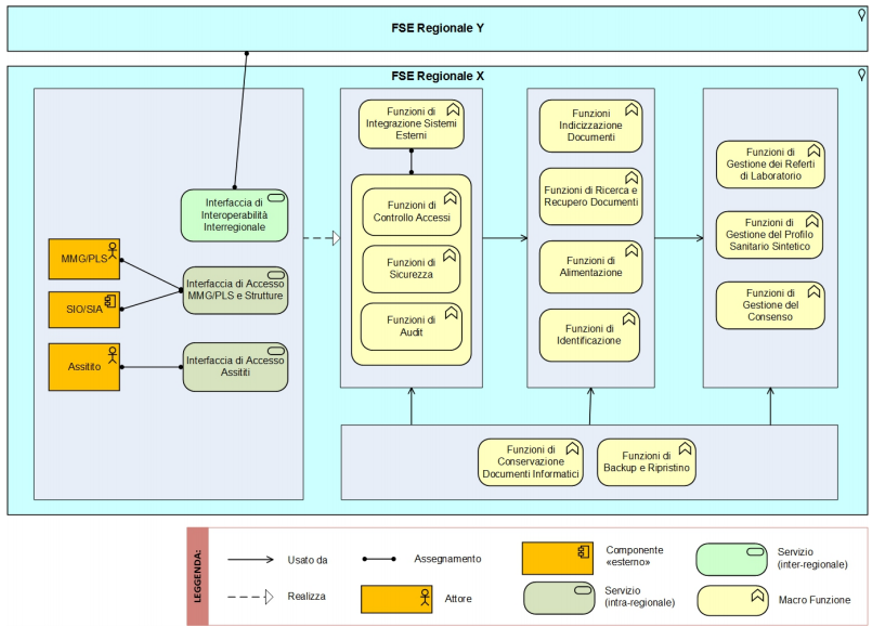
\includegraphics[width=.9\textwidth]{Sanitadigitale/fse}
		%
		\caption{Modello funzionale FSE}
		%
		\label{fig:modelloFSE}
		%
	\end{figure}
	%
\end{center}
%
Mentre le principali fonti di informazioni che il Fascicolo Sanitario Elettronico raccoglie sono le seguenti:
%
\begin{center}
	%
	\begin{figure}[tbhp]
		%
		\centering
		%
		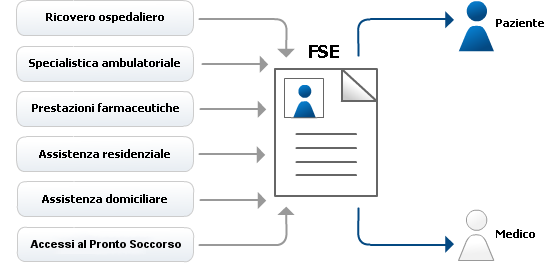
\includegraphics[width=.9\textwidth]{Sanitadigitale/fse2}
		%
		\caption{Schema dei dati raccolti dal FSE}
		%
		\label{fig:schema dati fse}
		%
	\end{figure}
	%
\end{center}
%
% In particolare nei servizi di interfaccia troviamo:
% \begin{itemize}
% 	\item \emph{Interfaccia di Interoperabilità Interregionale}: questa interfaccia rappresenta il punto di accesso ai servizi esposti dai sistemi regionali di FSE che consentono a questi ultimi di interoperare tra loro;
% 	\item \emph{Interfaccia di Accesso MMG/PLS e Strutture}: questa interfaccia consente alle strutture sanitarie e ai MMG/PLS di accedere ed utilizzare il sistema regionale di FSE;
% 	\item \emph{Interfaccia di Accesso Assistiti}: l’interfaccia offre la possibilità agli assistiti di accedere ed utilizzare il FSE;
% \end{itemize}
% Invece le macro funzioni sono state raggruppate nel seguente modo:
% \begin{enumerate}
% 	\item \emph{Funzioni di Integrazione Sistemi Esterni}: il sistema FSE deve predisporre una serie di funzioni che permettano l’utilizzo di servizi esposti da sistemi esterni, come ad esempio il servizio di anagrafe o il sistema di prenotazione delle prestazioni;
% 	\item \emph{Controllo Accessi}: tutti gli attori e le componenti esterne del sistema di FSE devono essere autenticate ed autorizzate da parte del sistema per poter accedere ed utilizzare i servizi messi a disposizione (funzioni di controllo accessi a livello regionale-nazionale);
% 	\item \emph{Sicurezza}: il sistema di FSE deve comprendere una serie di funzioni di supporto alla sicurezza, ad esempio per assicurare lo scambio sicuro dei dati e la tutela della privacy dell’assistito;
% 	\item \emph{Audit}: il sistema di FSE deve tracciare tutte le operazioni effettuate, mediante la memorizzazione e la gestione degli eventi di interesse;
% 	\item \emph{Funzioni Indicizzazione Documenti}: il sistema di FSE deve predisporre una serie di funzioni che consentano di indicizzare, mediante opportuni metadati, i documenti e dati prodotti dalle strutture sanitarie o socio-sanitarie (o condivisi dall’assistito);\footnote{I metadati hanno l’obiettivo di descrivere e di consentire il reperimento (mediante puntatori) dei documenti e dati prodotti sia all’interno che all’esterno del dominio regionale}
% 	\item \emph{Funzioni di Ricerca e Recupero Documenti}: i documenti e dati disponibili nel FSE devono essere facilmente reperibili da parte degli utenti autorizzati tramite opportune funzioni integrate nel sistema;
% 	\item \emph{Funzioni di Alimentazione}: il sistema di FSE deve mettere a disposizione funzioni che consentano agli attori autorizzati l’inserimento di dati e documenti nel sistema di FSE;
% 	\item \emph{Funzioni di Identificazione}: il sistema di FSE deve fornire una serie di funzioni per la gestione dell’identificazione dell’assistito, del professionista sanitario, del MMG/PLS e delle strutture sanitarie;
% 	\item \emph{Gestione Referti di Laboratorio}: il sistema di FSE deve fornire una serie di funzioni per la gestione dei referti di laboratorio;
% 	\item \emph{Gestione Profilo Sanitario Sintetico}: il sistema di FSE deve fornire funzioni atte alla gestione del Profilo Sanitario Sintetico;
% 	\item \emph{Gestione Consenso}: il sistema di FSE deve offrire una serie di funzionalità per la gestione di due tipologie di consenso da parte dell’assistito: consenso all’alimentazione e consenso alla consultazione dei dati e documenti del FSE;
% 	\item \emph{Backup e Ripristino}: il sistema di FSE deve fornire funzionalità trasversali a tutte le altre funzioni offerte, al fine di consentire la gestione di copie di sicurezza dei dati e documenti presenti nel FSE, la continuità ed il ripristino dei servizi erogati dai sistemi regionali.
% 	\item \emph{Conservazione Documenti Informatici}: il sistema di FSE deve rispettare le regole per la conservazione dei documenti e dati informatici (con riferimento ai documenti e dati di propria competenza, quali metadati componenti l’indice, informazioni condivise dall’assistito nel taccuino, dati relativi al consenso, ecc.), per il periodo di tempo previsto dalla normativa vigente;
% \end{enumerate}
La realizzazione di sistemi di FSE così strutturati costituisce, a livello regionale, un salto di notevole importanza per il miglioramento dell’efficacia ed efficienza delle cure percepite dai cittadini all’interno di un sistema sanitario regionale rispetto al modello precedente basato su registri e cartelle cartacee e blocchi di prescrizione stampati dalla zecca di Stato e consegnati personalmente ad ogni medico del distretto sanitario di appartenenza. \\
Una delle fonti di informazioni maggiori del Fascicolo Sanitario Elettronico, che è anche oggetto di studio in questo lavoro di tesi, risulta essere composta dall'insieme delle prescrizioni che i medici generano per i propri pazienti e che vengono erogate dalle farmacie presenti sul territorio nazionale. Il governo ha inoltre lasciato libertà di implementazione e gestione delle strutture alle singole regioni portando così alla creazione di sistemi eterogenei che fanno capo ad alcuni punti di riferimento gestiti dal Governo tramite le infrastrutture della Sogei. Il sistema complessivo si presenta come un sistema di tipo centralizzato caratterizzato dalle tipiche problematiche dei central points of failure. Inoltre, per quanto riguarda il sistema delle prescrizioni, esso gestisce solo le ricette mediche \emph{rosse} mentre le ricette mediche bianche non sono oggette ancora di prescrizione elettronica in tutte le regioni. Le funzionalità da cui si è partito per sviluppare questo lavoro di Tesi sono quelle riguardanti la prescrizione e l'erogazione delle ricette mediche \emph{bianche} che differiscono dalle ricette mediche rosse per una serie di caratteristiche che saranno illustrate nel proseguio del capitolo.
%
\section{Ricetta Elettronica}
%
Parallelamente al processo di istituzione del Fascicolo Sanitario Elettronico, anche il sistema di prescrizione farmaceutica è, al momento, oggetto di grandi modifiche in quanto sta diventando digitale. \\
Infatti, attraverso il \emph{Sistema Tessera Sanitaria} (TS), è stata realizzata la diffusione della ricetta elettronica, con la \gls{dematerializzazione} delle ricette mediche, introdotta con il D.L. n\degree 78/2010, il decreto ministeriale del 2/11/2011 ed il D.L. n\degree 179/2012. \cite{agendadigitale} Questo sistema è il sistema informativo centralizzato, realizzato in attuazione dell'art 50 del D.L. 269/2003, dal Ministero dell'economia e delle finanze - Ragioneria Generale dello Stato e gestito per la parte informatica da Sogei\footnote{Società di Information Technology interamente controllata dal Ministero dell'Economia e delle Finanze}.
La ricetta elettronica prevede la completa eliminazione del supporto cartaceo della ricetta nell’intero iter che va dalla fase di prescrizione del medico, alla erogazione della prestazione, al successivo controllo e rendicontazione. \\
Le finalità del progetto sono:
\begin{itemize}
	\item potenziamento dei controlli e prevenzione errori nelle prescrizioni;
	\item maggiore interscambio di informazioni favorito dal formato digitale;
	\item semplificazioni accesso prestazioni sanitarie a carico del SSN;
\end{itemize}
La prescrizione elettronica quindi, si presenta come il primo importante tassello nella costruzione del FSE in quanto rappresenta una delle porzioni più importanti dei dati clinici del paziente.\\
Esistono due tipi principali di ricette:
\begin{itemize}
	\item \emph{\gls{ricetta rossa}}: può essere compilata solamente dai medici dipendenti di strutture pubbliche o convenzionati con il servizio sanitario nazionale e viene utilizzata per la prescrizione di una terapia farmacologica, la prescrizione di un esame diagnostico o una visita specialistica a carico del servizio sanitario. L’uso di una ricetta rossa non permette l’erogazione a carico del servizio sanitario di farmaci o prodotti parafarmaceutici non compresi tra le formulazioni del prontuario farmaceutico regionale, né di esami, visite o terapie non comprese nei Lea o nelle disposizioni della propria regione. Un esempio è illustrato nella seguente figura:
	      %
	      \newline
	      %
	      \begin{figure}[h!]
	      	%
	      	\centering
	      	%
	      	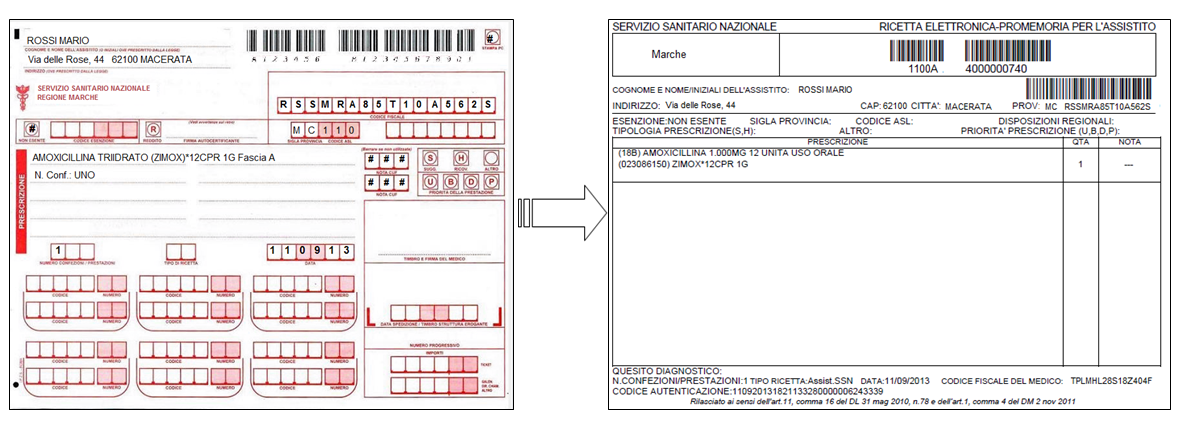
\includegraphics[width=1.0\textwidth]{Sanitadigitale/ricetta}
	      	%
	      	\caption{Ricetta rossa dematerializzata}
	      	%
	      	\label{fig:Ricetta rossa dematerializzata}
	      	%
	      \end{figure}
	      %
	      \newline
	      %
	\item \emph{\gls{ricetta bianca}}: ricetta che il medico compila su carta bianca, sulla quale siano però riportati: il nome e cognome del medico; la data; il luogo; la firma autografa del medico. In questo caso, il nome dell’assistito non è strettamente necessario. Su ricetta bianca possono essere prescritte tutte le prestazioni di specialistica ambulatoriale, di diagnostica strumentale e di laboratorio, di norma correlate alla propria branca di specializzazione e i farmaci, prestazioni che saranno sempre a carico del cittadino assistito. Per la prescrizione a carico del servizio sanitario è infatti necessaria la ricetta del ricettario regionale ed è valida in tutte le farmacie italiane. Una delle attuali criticità del sistema è che il procedimento della dematerializzazione delle ricette non si applica per le ricette bianche che vengono ancora compilate su normale carta:
	      \begin{center}
	      	%
	      	\begin{figure}[tbhp]
	      		%
	      		\centering
	      		%	      		      	
	      		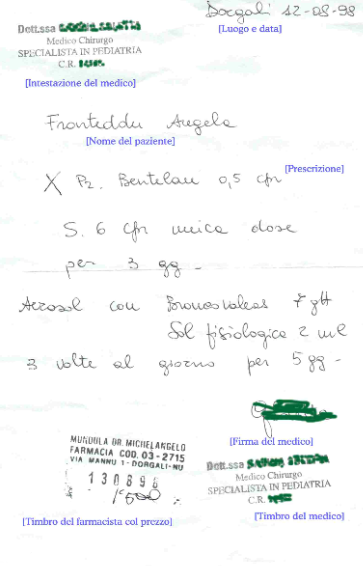
\includegraphics[width=0.5\textwidth]{Sanitadigitale/ricettaBianca}
	      		%
	      		\caption{Ricetta bianca}
	      		%
	      		\label{fig:Ricetta bianca}
	      		%
	      	\end{figure}
	      	%
	      \end{center}
\end{itemize}
%
\section{Architettura del Sistema}
%
L'attività di accoglienza dei dati delle ricette prescritte, prevede l'utilizzo di due sistemi centrali:
\begin{enumerate}
	\item \emph{Sistema di accoglienza} (SAC): è il Sistema di Accoglienza Centrale gestito da Sogei per il Ministero dell'Economia e delle Finanze (MEF). Il SAC gestisce la circolarità nazionale delle ricette dematerializzate, ovvero la possibilità per gli assistiti di utilizzare una prescrizione in qualunque Regione, garantendo anche che la stessa prestazione non sia erogata più volte in regioni diverse;
	\item \emph{Sistema di accoglienza regionale} (SAR): è il Sistema di Accoglienza Regionale gestito da CUP 2000 che colloquia con il Sistema di Accoglienza Centrale del Ministero (SAC) per l’invio e il recupero delle ricette dematerializzate, ed aggiorna lo stato della ricetta (prenotata, sospesa,bloccata ed erogata) E' in grado di: \begin{itemize}
	\item raccogliere tutte le prescrizioni dematerializzate inviate dai medici prescrittori della Regione;
	\item rendere disponibili le prescrizioni dematerializzate ai sistemi che, se abilitati, possono accedere alla ricetta stessa (CUP, accettazioni, farmacie, etc.);
	\item fornire servizi di ritorno informativo verso le Aziende sanitarie e le farmacie;
	\item sviluppare le regole e i controlli regionali necessari a garantire l’emissione di prescrizioni corrette;
	\end{itemize}
\end{enumerate}
Questi due sistemi coesistono contemporaneamente, in quanto nel caso in cui le regioni non avessero sviluppato un proprio sistema di accoglienza, il SAC si configura come sistema di riferimento per i medici prescrittori, le farmacie e le strutture di erogazione di prestazioni di specialistica ambulatoriale, generando per questi le credenziali di accesso al sistema\footnote{abilitazione al SAC. Credenziali inviate tramite busta chiusa alle ASL territoriali}. Invece nel caso in cui la regione abbia a disposizione un SAR proprio, esso si andrà ad interfacciare con il SAC, che fungerà da secondo centro di accoglienza con le stesse funzionalità del SAR, solamente estese a livello nazionale.
%
\subsection{Caso di studio: Regione Marche}
%
Nella Regione Marche, la delibera 677\cite{drmarche} della Giunta Regionale 04/06/2014 per l'approvazione dello "schema di protocollo di intesa con i medici di medicina generale per la riqualificazione della medicina del territorio e la messa a regime della rete regionale per la ricetta dematerializzata e per l'implementazione dei flussi di dati" che ha dato il via al progetto di dematerializzazione delle ricette SSN il quale prevede la sostituzione della ricetta rossa cartacea con la ricetta elettronica dematerializzata. La procedura per l'emissione di una ricetta è la seguente:
\begin{itemize}
	\item il medico prescrittore:
	      \begin{enumerate}
	      	\item si collega al Sistema Centrale Tessera Sanitaria (anche attraverso un eventuale SAR)\footnote{essendo nelle Marche presente anche il SAR, la comunicazione avviene verso il SAR e poi verso il SAC e successivamente viene effettuato un controllo incrociato delle informazioni inserite nei due sistemi};
	      	\item genera i dati della ricetta elettronica. Il contenuto della ricetta viene salvato nel Sistema Tessera Sanitaria a livello centrale (tenuto sempre conto che il contenuto sarà anche salvato nel SAR, se presente). La ricetta sarà identificata tramite un codice univoco nazionale denominato \emph{Numero di Ricetta Elettronica} (NRE) e conterrà i seguenti elementi: NRE, dati anagrafici dell'assistito titolare della prescrizione, eventuali esenzioni e la prestazione da erogare;
	      	\item se i dati risultano corretti, il medico rilascia al paziente un \emph{promemoria} cartaceo contenente i dati della ricetta dematerializzata;
	      \end{enumerate} 
	\item la struttura erogatrice:
	      \begin{enumerate}
	      	\item presso la struttura erogatrice, l'assistito presenterà il promemoria;
	      	\item la struttura si collegherà al sistema centrale (SAR o SAC) e procederà alla ricerca della ricetta attraverso l'NRE riportato su di essa, unitamente al codice fiscale dell'assistito riportato sulla sua tessera sanitaria;
	      	\item nel caso in cui la ricetta risulti erogabile, la struttura procede all'erogazione della prestazione comunicando al tempo stesso le informazioni sulla prestazione erogata (al SAR e/o al SAC);
	      	\item completata l'erogazione la struttura ritira il promemoria al paziente;
	      \end{enumerate}
\end{itemize}
Questa sequenza viene mostrata nella figura seguente:
%
\begin{figure}[H]
	%
	\centering
	%
	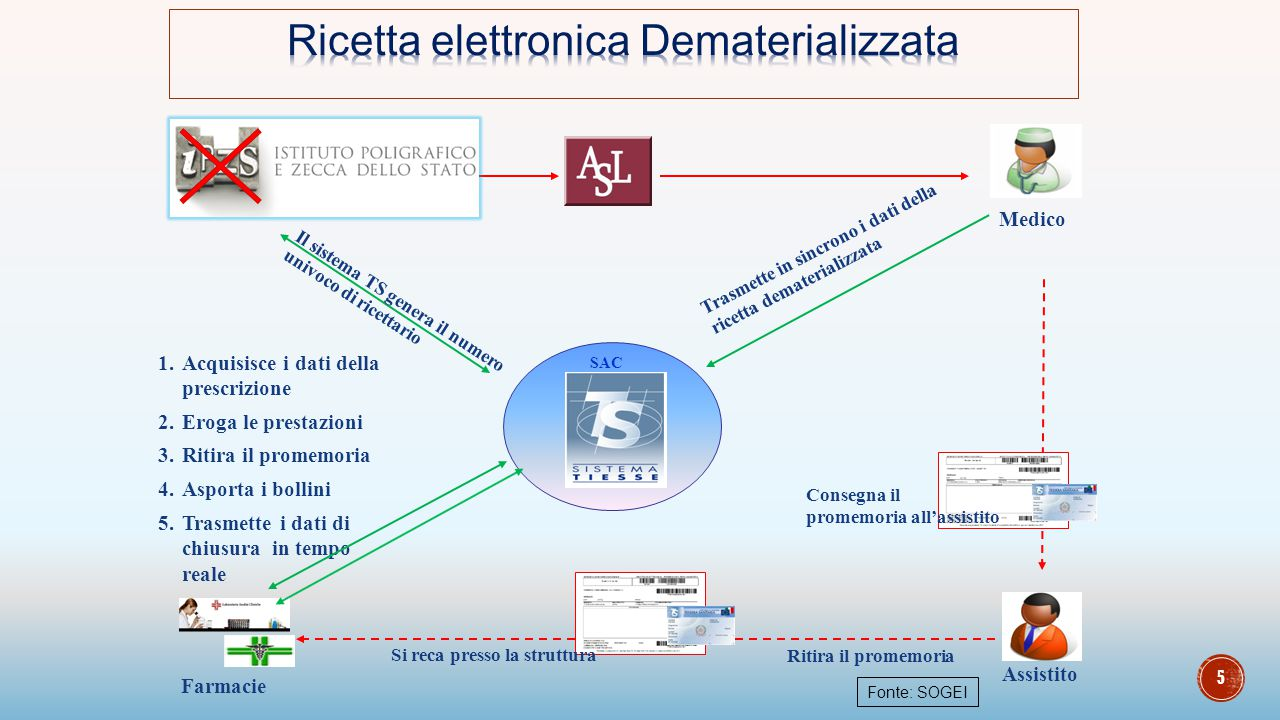
\includegraphics[width=.9\textwidth]{Sanitadigitale/erogazioneRicetta}
	%
	\caption{Diagramma dell'erogazione di una ricetta}
	%
	\label{fig:Erogazione di una ricetta dematerializzata}
	%
\end{figure}
%
Il complesso dei servizi offerti dal FSE nell'ambito della Regione Marche è garantito da un insieme di componenti applicative cooperanti tra loro supportate da un apparato infrastrutturale allocato presso il data center sanità e i nodi aziendali, il tutto integrato all’interno di un contesto regionale caratterizzato dall’esistenza di sistemi preesistenti, con cui il FSE si troverà ad interagire  per l’esposizione dei propri servizi rispetto al SAC centrale. Le componenti sono eterogenee e sono riassunte nella seguente figura:
%
\begin{figure}[H]
	%
	\centering
	%
	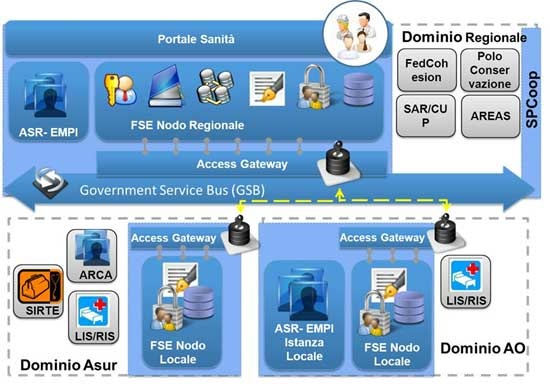
\includegraphics[width=.9\textwidth]{Sanitadigitale/sanitaMarche}
	%
	\caption{Schema architetturale sanità digitale Marche}
	%
	\label{fig:Schema architetturale sanità digitale Marche}
	%
	\vfill
\end{figure}
%
\section{Una soluzione decentralizzata}
%
\subsection{Criticità del sistema}
Questo sistema ha dimostrato alcune criticità a seguito delle sperimentazioni fatte e dell'attuale utilizzo:
\begin{itemize}
	\item la mancanza di collegamenti internet o di una piattaforma di gestione troppo lenta in alcune zone crea problemi di utilizzo e di sovraccario del sisstema;
	\item la presenza di due distinti sistemi di trasmissione dati e accoglienza delle ricette (SAC/SAR) ha aggiunto un ulteriore grado di complessità alle architetture dei sistemi a livello regionale ed inter-regionale in quanto alcune regioni hanno optato per l'utilizzo del SAC mentre altre del SAR (che si interfaccia con il SAC). Inoltre, normalmente un SAR risulta essere più lento di un SAC a livello di gestione del flusso dei dati;
	\item la prescrizione delle ricette bianche risulta essere esclusa dalla dematerializzazione. Quindi una ricetta bianca può essere oggetto di falsificazione o truffa, nel caso in cui il blocco di ricette con i dati del medico venga rubato;
\end{itemize}
Inoltre, possono verificarsi casi in cui i server di Sogei del SAC responsabili della prescrizione e spedizione della ricetta digitale risultino irragiungibili con conseguenze che vanno dal mancato invio della ricetta digitale al non poter verificare la veridicità del contenuto di un promemoria se non in modo "postumo" all'erogazione del contenuto della prescrizione cartacea.
%
\subsection{La decentralizzazione}
Una possibile soluzione di queste criticità può essere trovata nell'utilizzo di un approccio decentralizzato che risiede nell'utilizzo della blockchain (si eliminano i Single Point of Failure) per registrare gli eventi (che saranno organizzati in blocchi) e le transazioni di prescrizione ed erogazione.  L'utilizzo della blockchain ci garantisce:
\begin{itemize}
	\item \emph{Non ripudio}: la decisione riguardante la validità di un’informazione non viene presa unilateralmente ma attraverso un meccanismo di raccolta del consenso all’interno della rete, rendendo così particolarmente difficile metterne in discussione l’esito;
	\item \emph{Autenticità}: tutti gli eventi possono essere fatti risalire con certezza alle identità digitali che li hanno generati, attraverso l’utilizzo di meccanismi di crittografia asimmetrici;
	\item \emph{Integrità}: i dati che sono stati scritti all’interno della Blockchain non possono essere modificati, se non attraverso specifiche regole del protocollo che definiscono rigorosamente le modalità con cui si possono effettuare cambiamenti;
	\item \emph{Tracciabilità}: a tutti gli eventi registrati vengono assegnati un identificativo e una marca temporale che li rende facilmente tracciabili e verificabili.
	\item \emph{Programmabilità}: all’interno dei blocchi possono essere incluse istruzioni che facciano scatenare specifiche azioni al verificarsi certe condizioni.
\end{itemize}

%
% ------------------------------------------------------------------------ %
% !TEX encoding = UTF-8 Unicode
% !TEX TS-program = pdflatex
% !TEX root = ../Tesi.tex
% !TEX spellcheck = it-IT
% ------------------------------------------------------------------------ %
%
% ------------------------------------------------------------------------ %
% 	NOME CAPITOLO
% ------------------------------------------------------------------------ %
%
\chapter{Blockchain}
%
\label{cap:blockchain}
%
\section{Introduzione}
Una blockchain è una base di dati distribuita organizzata in blocchi, ciascuno dei quali contiene un insieme di record. Questi ultimi rappresentano la registrazione di un particolare evento associato ad un istante temporale (un timestamp). La struttura complessiva della rete assume la forma di una catena poichè ciascun blocco è legato al precedente, come è illustrato nella seguente immagine:
\begin{center}%
	\begin{figure}[h!]
		%
		\centering
		%
		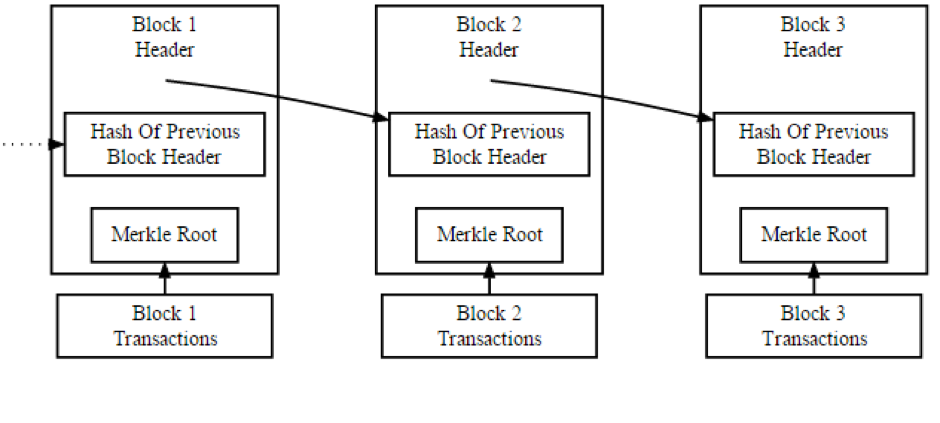
\includegraphics[width=.95\textwidth]{Blockchain/bloccoBlockchain}
		%
		\caption{Catena di blocchi in una blockchain}
		%
		\label{fig:catena di blocchi in una blockchain}
		%
	\end{figure}%
\end{center}
Il legame tra un blocco ed il suo predecessore viene realizzato attraverso l'inserimento, in ciascun blocco, di un riferimento al blocco precedente. Questa dipendenza all'indietro trova la sua conclusione nel blocco iniziale della catena, che solitamente viene generata da zero. Questa tecnologia nasce come infrastruttura della criptovaluta conosciuta come \emph{Bitcoin}, il cui fondatore, noto con lo pseudonimo di Satoshi Nakamoto, l'ha creata nel 2009 generando il primo blocco dopo aver spiegato il funziomento del sistema nel suo documento pubblicato un anno prima. \cite{bitcoin} \\
Ma questa non è l'unica definizione che si può dare della blockchain in quanto ogni definizione può mettere  in evidenza uno o più aspetti salienti della tecnologia stessa.
%
\paragraph{Blockchain come evoluzione del concetto di \enquote*{Ledger}} 
Con \emph{Ledger} si intende il \enquote*{libro mastro} in cui vengono registrate tutte le transazioni del sistema. Sotto quest'ottica la Blockchain è la realizzazione del \emph{Distributed Ledger}, come evoluzione dal \emph{Centralized Ledger}, passando per il \emph{Decentralized Ledger}. Tipicamente, la logica centralizzata è rappresentata dal tradizionale \enquote*{Centralized Ledger} con un rapporto rigorosamente centralizzato \enquote*{Uno-A-Tanti}, dove tutto deve essere gestito facendo riferimento a una struttura o autorità o sistema centralizzato. Nel Centralized Ledger la fiducia è nell’autorità, nell’autorevolezza del soggetto o sistema che rappresenta il \enquote*{centro} dell’organizzazione. \\
Dal modello centralizzato, si passa attraverso il \enquote*{Decentralized Ledger}, che ripropone la logica della centralizzazione a livello \enquote*{locale} con \enquote*{satelliti} organizzati a loro volta nella forma di Uno-A-Tanti che si relazionano a loro volta in una forma che ripete il modello Uno-A-Tanti. Non c’è più un \enquote*{grande} soggetto centrale ma ci sono tanti \enquote*{soggetti centrali}. La fiducia anche in questo caso viene delegata a un soggetto centrale, logicamente più vicino, ma comunque centralizzato. Le organizzazioni basate su Decentralized Ledger definiscono una Governance che stabilisce delle forme di coordinamento di tipo centralizzato. \\
Infine si arriva al \enquote*{Distributed Ledger}, ovvero ad una reale e completa logica distribuita dove non esiste più nessun centro e dove la logica di governance viene costruita attorno a un nuovo concetto di fiducia tra tutti i soggetti. Il processo decisionale passa attraverso un rigoroso processo di costruzione del Consenso.
%
\begin{center}%
	\begin{figure}[H]
		%
		\centering
		%
		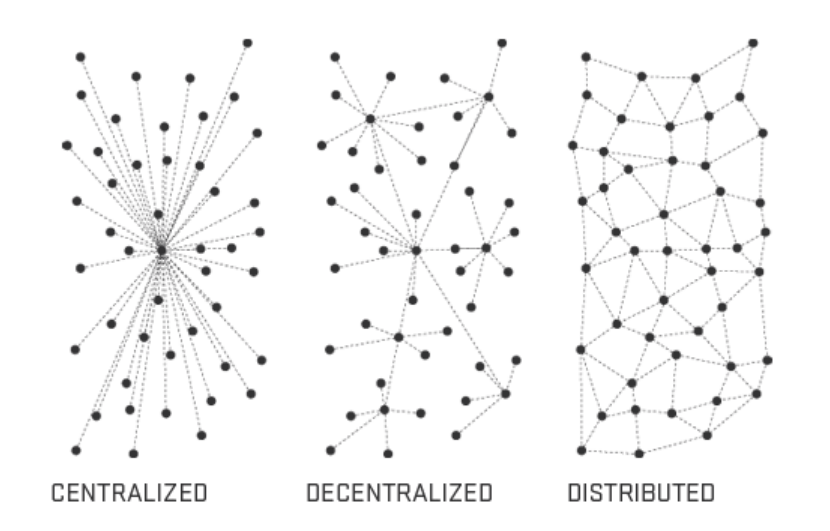
\includegraphics[height=5cm,width=.85\textwidth]{Blockchain/cdd}
		%
		\caption{Da Centralized a Decentralized Ledger}
		%
		\label{fig:da centralized a decentralized ledger}
		%
	\end{figure}%	
\end{center}
%
\section{Caratteristiche Generali}
%
La blockchain si evolve attraverso l'attività di un timestamp server distribuito, che prende un blocco di item e tramite la Marca Temporale\footnote{istante temporale o timestamping} marca il blocco e ne calcola l'hash. Mentre nei centralized ledger il punto di forza era localizzato nella fiducia che tutti i partecipanti dovevano avere nel gestore del central ledger (un soggetto di terze parti al di sopra dei partecipanti che garantisce la fiducia), nel distributed ledger la blockchain può essere considerata come una base di dati senza intermediari, ovvero che per utilizzarla non è necessario rivolgersi ad un server. Infatti le sue caratteristiche e la sua natura decentralizzata sono quelle che garantiscono l'affidabilità e la fiducia senza la presenza di un’autorità centrale che regoli le attività dei vari utenti. Questo ad esempio, nel caso di Bitcoin, si traduce nell'eliminazione di entità bancarie in grado di controllare (ed eventualmente anche alterare) le transazioni. \\
Una blockchain gode quindi delle seguenti proprietà:
\begin{enumerate}
	\item è distribuita: le informazioni sono replicate e dislocate su più nodi della rete;
	\item è inviolabile: essendo i blocchi condivisi tra più nodi ed dato che, per alterarne il contenuto è necessario il consenso della maggioranza assoluta, è improbabile che un attacco vada a buon fine;
	\item può essere pubblica (Unpermissioned Ledger) dove chiunque può controllare l'attività di chiunque, ma può anche essere privata (Permissioned Ledger) dove i partecipanti alla blockchain sono un numero limitato di attori che sono definiti come trusted. Le \gls{permissioned} sono più vicine alle esigenze di imprese ed istituzioni che vogliono comunque servirsi della tecnologia della blockchain;
	\item rispetta i requisiti di:
	      \begin{itemize}
	      	\item \emph{confidenzialità}: le informazioni sono accessibili solo agli utenti autorizzati;
	      	\item \emph{integrità}: ognuno può alterare solo i dati per cui è autorizzato;
	      	\item \emph{non ripudio}: le transazioni irrevocabili (caratteristica fondamentale della blockchain);
	      	\item \emph{autenticità}: vengono utilizzati meccanismi di cifratura per garantire l'autenticità nella blockchain.
	      \end{itemize}%
\end{enumerate}
%
\section{Architettura}
%
L'architettura di una blockchain (semplificata), può essere osservata nella seguente figura:
% \begin{center}
\begin{figure}[H]
	%
	\centering
	%
	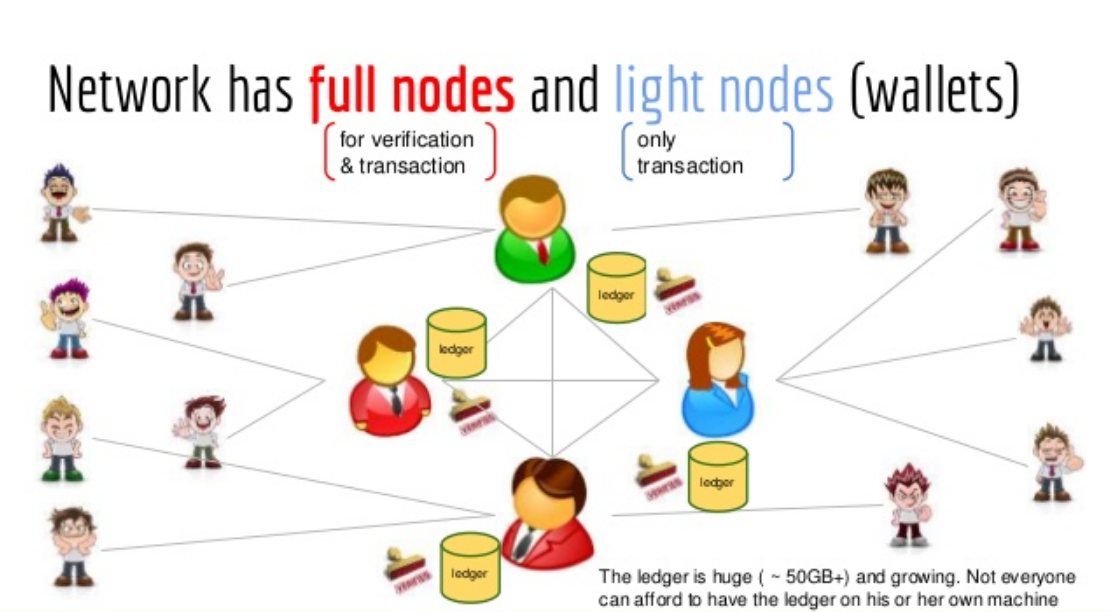
\includegraphics[width=.9\textwidth]{Blockchain/node}
	%
	\caption{Architettura di una blockchain su cui operano full node e lightweight node}
	%
	\label{fig:architettura di una blockchain}
	%
\end{figure}
%	
% \end{center}
Possiamo notare come l'assenza di intermediari si rispecchi a livello architetturale. Infatti la rete su cui si basa questa tecnologia è di tipo "peer to peer". Questa architettura risulta essere scalabile, dato che ciascun nodo può essere rimosso dalla rete o aggiunto alla stessa senza che l'attività complessiva risulti compromessa. Un nodo, per unirsi alla blockchain, ha due possibilità:
\begin{enumerate}
	\item diventare un \emph{full node}: il nodo deve scaricare una copia della blockchain al fine di poter effettuare operazioni e, al tempo stesso, validare le operazioni effettuate dagli altri utenti della blockchain;
	\item diventare un \emph{lightweight node}: il nodo può comunque partecipare alle attività della blockchain, senza però validare le operazioni degli altri utenti. Il vantaggio di un lightweight node risiede nel fatto che non deve scaricare l'intera copia della blockchain (ne scarica solamente una parte) per poter compiere delle operazioni ma agisce interrogando esso stesso uno dei full node presenti nella rete.
\end{enumerate}
%
\section{Mining e Proof of Work}
Il processo di consenso decentralizzato del Bitcoin richiede l'esistenza dei nodi nel network che continuamente tentano di produrre pacchetti di transazioni chiamati \enquote*{blocchi}. Il network produce all'incirca un blocco ogni dieci minuti ed ogni blocco contiene, come abbiamo detto in precedenza, una marca temporale, un numero casuale(nonce), un riferimento al precedente blocco (l'hash del precedente blocco) e una lista di tutte le transazioni che sono avvenute dal precedente blocco. Con il passare del tempo si crea quindi una persistente, sempre crescente catena che si aggiorna costantemente per rappresentare l'ultimo stato del libro mastro di Bitcoin. \\ 
Questo processo di creazione di un nuovo blocco va sotto il nome di \emph{mining} e viene realizzato da entità facenti parte della rete chiamate \emph{miners}. Per generare un blocco generalmente è necessario:
\begin{itemize}
	\item stabilire quali transazioni andranno a far parte del nuovo blocco;
	\item verificare la validità di queste transazioni;
	\item selezionare il blocco più recente della blockchain (l'ultimo creato) ed inserire il suo hash nel nuovo blocco;
	\item risolvere infine la \emph{Proof-of-work} (POW) e, contemporaneamente, assicurarsi che eventuali blocchi generati prima del proprio siano validi.
\end{itemize}
La componente principale dell'attività di mining è la fase che riguarda la Proof-of-work, ovvero quella che involve tutti i miners e che li vede impegnati nella risoluzione di un problema ad elevata complessità (in cui è richiesta un'elevata capacità di calcolo), la cui risoluzione avrà come risultato l'aggiunta di un nuovo blocco alla rete e un pagamento in Bitcoin al miner che ha risolto il blocco. La POW si articola nel seguente modo: viene utilizzato l'algoritmo di hash SHA-256 che produce un numero formato da 256 bit. L'oggetto su cui si applica la funzione di hash, costituito dal blocco di transazioni corrente, è il cosiddetto \emph{header}\footnote{comprende il numero di versione del protocollo, l’hash del blocco precedente, l’hash di un sommario delle transazioni del blocco corrente, una timestamp (cioè data e ora di creazione del blocco) e il grado di difficoltà stabilito per il blocco corrente blocco e il nonce} del blocco. L'obiettivo di questa sfida è ottenere un valore di hash inferiore di un target regolato dinamicamente\footnote{generalmente il target viene ricalibrato dal network ogni 2016 blocchi, al fine di lasciar costante il tempo di produzione di un blocco (10 minuti)}. Poichè SHA-256 è progettato peressere una funzione completamente imprevedibile e pseudo-randomica, l'unico modo per creare un blocco valido è un insieme di tentativi con l'incremento ripetuto del nonce al fine di trovare il valore richiesto dalla proof-of-work. Si nota come questa sfida computazionale sia difficile da completare ma facilmente verificabile all'interno della rete. \\
Una volta risolta la proof-of-work e generato il blocco associato, per alterare una transazione in un blocco, bisognerebbe modificare anche tutte le transazioni passate (essendo esse collegate in cascata da una serie di firme digitali) e rimettere quindi in gioco tutta la capacità di calcolo utilizzata nella risoluzione perchè si dovrebbe rimodificare quel blocco e tutti i suoi successori. Infine al minatore che ha risolto il blocco generato viene ricompensato con una certa quantità di bitcoin. In altre implementazioni della blockchain esistono altri strumenti per stabilire chi andrà a minare il blocco successivo:
\begin{itemize}
	\item \emph{proof-of-stake}: il diritti di minare viene concesso in funzione della quantità di denaro che si possiede (adatta in contesti con bassa capacità di calcolo);
	\item \emph{prrof-of-burn}: il miner può  aggiudicarsi la contesa dimostrando di aver consumato monete, inviandole ad un indirizzo non suo e non potendole quindi più utilizzare, dimostrando di aver fatto un sacrificio.
\end{itemize}
%
\section{Le transazioni}
%
Una transazione rappresenta un trasferimento di valore che viene registrato in un blocco della blockchain. Bitcoin, ad esempio, utilizza un sistema di transizioni di stato dove:
\begin{itemize}
	\item stato: consistente nella proprietà dello status di tutti i bitcoins esistenti;
	\item funzione di transizione di stato: riceve uno stato ed una transizione e trasmette un nuovo stato che ne costituisce il risultato.
\end{itemize}
In bitcoin lo \enquote*{stato} è la raccolta di tutte le monete (tecnicamente definite come \enquote*{transazioni in uscita non spese} o UTXO\footnote{Unspend Transaction Output}). Ogni UTXO ha una denominazione ed un proprietario definito da un indirizzo di 20 byte che corrisponde essenzialmente alla sua chiave pubblica. Una transazione viene costruita in riferimento a transazioni passate da cui prelevare i fondi che vengono trasferiti al nuovo destinatario. Quindi ogni transazione contiene:
\begin{itemize}
	\item uno o più vettori di input, dove ogni input contiene un riferimento ad uno UTXO esistente ed una firma crittografica prodotta da una chiave privata associata all'indirizzo del proprietario\footnote{in questo modo si evita la possibilità che una persona spenda monete non di sua proprietà};
	\item uno o più vettori di output, dove ogni output contiene un nuovo UTXO che deve essere aggiunto allo stato;
\end{itemize}
Una transazione può avvenire nel seguente modo:
\begin{center}
	\begin{figure}[H]
		%
		\centering
		%
		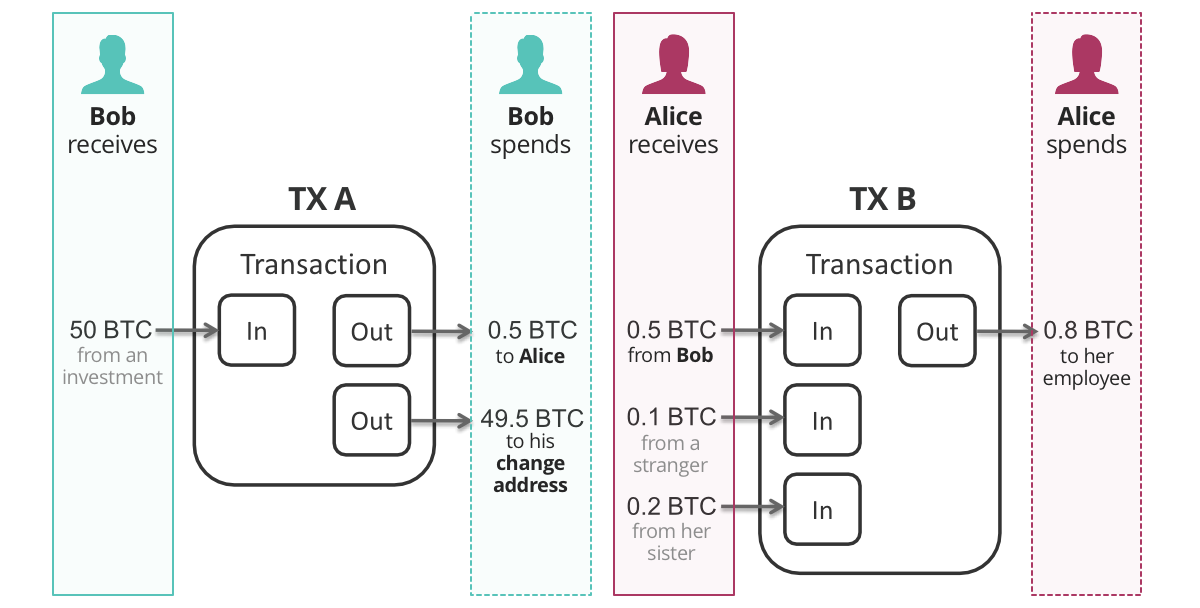
\includegraphics[width=.9\textwidth]{Blockchain/bitcoinTransaction}
		%
		\caption{Esempio di transazione}
		%
		\label{fig:esempio di transazione}
		%
	\end{figure}
\end{center}
%
Ogni transazione effettuata viene quindi inviata a tutti i nodi i quali raccolgono le nuove transazioni in un blocco e partecipano alla proof-of-work per minare il nuovo blocco. Un blocco, per essere accettato deve contenere al suo interno solamente transazioni valide e non deve essere presente il problema del \emph{double spending} (spendere gli stessi soldi due volte).
%
\section{Permissioned Blockchain}
%
Sono attualmente presenti numerosi progetti di blockchain permissioned, come il progetto Hyperledger\cite{website:hyperledger} della Linux Foundation, o la rete Gem Health\cite{gem}. Alcuni ritengono che le blockchain private siano sono un modo alternativo di definire uno shared-database. Infatti, come sostenuto da Gideon Greenspan, CEO di CoinSciences :"se fiducia e robustezza non sono un target, non c'è nulla che una blockchain possa fare ed un database no", a conferma del fatto che le due tecnologie sono tutto sommato alternative, ma non analoghe.\\
Nel presente lavoro di tesi, verrà utilizzata una blockchain \emph{permissioned} (privata). Una blockchain permissioned gode innanzitutto delle stesse proprietà di una blockchain pubblica, ovvero:
\begin{itemize}
	\item è una rete peer-to-peer decentralizzata dove ogni partecipante mantiene una replica di un libro mastro di transazioni firmate digitalmente;
	\item le repliche sono mantenute sincronizzate attraverso un protocollo di consenso;
	\item sono presenti garanzie di immutabilità anche in presenza di partecipanti maligni.
\end{itemize}
Quello che una blockchain permissioned aggiunge ad una blockchain pubblica è un meccanismo di controllo degli accessi integrato nei client, così che i peer possano essere aggiunti nella rete sulla base di un valore di controllo (un certificato o un indirizzo ad esempio). La scelta di utilizzare blockchain permissioned si adatta alla volontà di aziende, governance e pubbliche amministrazioni che vogliono utilizzare il livello tecnlogico e la sicurezza raggiunte dalle blockchain, mantenendo al tempo stesso la loro presenza all'interno della rete, necessaria per mantenere il controllo sui partecipanti. Queste blockchain sono sì adatte a gestire moneta, ma le loro potenzialità si manifestano soprattutto in altri campi come la condivisione di dati medicali (i quali non devono essere alterati in alcun modo) o la catena di distribuzione di farmaci (per evitare frodi a qualsiasi livello della supply-chain, dalla produzione alla vendita al dettaglio). \\
Le blockchain permissioned imitano il processo di sicurezza utilizzato dalle blockchain pubbliche come Bitcoin, ma essendo il numero e l'identità dei partecipanti conosciuto, non c'è il bisogno della proof-of-work o della proof-of-stake, mentre utilizzano la stessa crittografia e le stesse strutture dati come i Merkle trees\cite{merkle} per assicurare che transazioni non valide non siano aggiunte alla blockchain. I meccanismi di consenso più popolari includono Raft\cite{raft} e Juno\cite{juno}. Questi protocolli di consenso funzionano sulla base di un modello leader-follower, in cui per ogni blocco viene selezionato un leader che crea il blocco e lo aggiunge alla blockchain, mentre errori ed anomalie vengono automaticamente corretti dal sistema. \\
Anche le blockchain permissioned godono della robustezza tipica della loro controparte pubblica dato che mantengono la proprietà di essere ridondanti e quindi estremamente fault-tolerant. Ogni nodo processa le transazioni, perciò nessun nodo risulta indispensabile. Per questo motivo, e per la natura peer-to-peer della rete, la replicazione che nei database viene realizzata tramite tecniche apposite, nelle blockchain è un processo naturale dato che i nodi si sincronizzano a vicenda. Infine ogni volta che si effettua una transazione rispetto ai database tradizionali, i sistemi basati su blockchain devono farsi carico di ulteriori oneri:
\begin{itemize}
	\item verifica della firma: ogni transazione deve essere firmata con uno schema di crittografia a chiave pubblica;
	\item meccanismo di conenso: i nodi della rete devono raggiungere il consenso;
	\item ridondanza delle operazioni.
\end{itemize}
Questo ovviamente si traduce in prestazioni minori rispetto ai database tradizionali.\\
Le blockchain permissioned quindi cercano di unire le capacità di prestazione e riservatezza (tipiche dei database tradizionali) con i meccanismi di fault-tolerance e disintermediazione (per quanto possibile nelle blockchain private) tipiche della blockchain.
%
\section{Limiti delle Blockchain}
%
Per quanto valida la tecnologia della blockchain come quella presentata ed implementata da Bitcoin, essa presenta dei limiti nel caso in cui si voglia costruire applicazioni avanzate su di essa. Infatti Bitcoin presenta un linguaggio di scripting estremamente limitato, che soffre dei seguenti limiti:
\begin{enumerate}
	\item \emph{mancanza di completezza del linguaggio di Turing}: ovvero, mentre esiste un grande sottoinsieme di calcolo che il linguaggio di scripting del Bitcoin supporta, quest ultimo non supporta tutto. Infatti troviamo la mancanza dei \enquote{loop};
	\item \emph{cecità del valore}: non c'è un modo per un UTXO di fornire un controllo a setaccio sull'ammontare ritirabile;
	\item \emph{mancanza di stato}: UTXO può essere sia speso che non speso, non c'è possibilità per scripts di mantenere altri stati interni oltre questo.
\end{enumerate}
La soluzione sta nelle blockchain di seconda generazione che riprendono un concetto teorizzato negli anni '70, gli Smart Contract, e lo implementano all'interno della loro rete peer-to-peer.
%

%
% ------------------------------------------------------------------------ %
% !TEX encoding = UTF-8 Unicode
% !TEX TS-program = pdflatex
% !TEX root = ../Tesi.tex
% !TEX spellcheck = it-IT
% ------------------------------------------------------------------------ %
%
% ------------------------------------------------------------------------ %
% 	NOME CAPITOLO
% ------------------------------------------------------------------------ %
%
\chapter{Ethereum}
%
\label{cap:ethereum}
%
% ------------------------------------------------------------------------ %
%
\section{Introduzione e Smart Contracts}
%
Gli Smart Contract sono stati oggetto di sperimentazione già negli anni ’90 quando le tecnologie hanno permesso di attuare forme di sperimentazione di Smart Contract, ma l’idea di Contratto Intelligente risale in realtà alla metà degli Anni ’70. Il termine adottato all’epoca non era quello di Smart Contract, ma il concetto era sostanzialmente quello che ha portato ai contratti intelligenti. Infatti all’epoca l’esigenza atteneva alla necessità di gestire l'attivazione o disattivazione di una licenza software in funzione di alcune condizioni molto semplici. La licenza di determinati software venne di fatto gestita da una chiave digitale che permetteva il funzionamento del software se il cliente aveva pagato la licenza e ne cessava il funzionamento alla data di scadenza del contratto è stato il primo esempio di uno Smart Contract. \\
\emph{Ethereum}\autocite{eth} nasce invece nel 2013 per opera di Vitalik Buterin, uno sviluppatore di origini russe che ha unito la sua competenza di programmatore a quelle di ricercatore nell’ambito delle cryptocurrency. Lo scopo di Ethereum è quello di creare un protocollo alternativo per la costruzione di applicazioni decentralizzate in situazioni in cui sono essenziali: un tempo rapido di sviluppo, un alto gradi di sicurezza nelle applicazioni e la capacità di far interagire tra di loro in modo efficace applicazioni differenti. In definitiva, Ethereum è una blockchain con un linguaggio di programmazione costruito al suo interno, Turing completo, che permette a chiunque voglia di scrivere Smart Contracts e applicazioni decentralizzate (o DAPP) nelle quali è possibile stabilire:
\begin{itemize}
	\item le proprie regole di proprietà;
	\item i formati delle transazioni;
	\item le funzioni di transizione di stato.
\end{itemize}%
L’uso delle risorse computazionali di Ethereum è remunerato con una speciale “moneta virtuale” denominata \emph{Ether} che rappresenta essa stessa sia la potenza elaborativa necessaria per produrre i contratti sia la cryptovaluta che permette di “pagare” per la realizzazione dei contratti\footnote{in maniera simile a quanto avviene sulla blockchain di Bitcoin}. Ether è fondamentalmente un token che viene trattato come cryptocurrency exchange con il ticker symbol di ETC. \\
Una generica applicazione Ethereum decentralizzata può essere schematizzata ad alto livello nel seguente modo: 
\begin{center}%
	\begin{figure}[H]
		%
		\centering
		%
		\includegraphics[width=.9\textwidth]{Ethereum/dapp}
		%
		\caption{Esempio di applicazione decentralizzata}
		%
		\label{fig:esempio di dapp}
		%
	\end{figure}
	%
\end{center}%
\section{Ethereum Accounts} 
%
In Ethereum, lo stato è costituito da oggetti chiamati \enquote*{accounts}. Ognuno di essi ha un indirizzo di 20 byte e le transizioni di stato sono trasferimenti diretti del valore e dell'informazione tra gli accounts. Un account Ethereum, è composto dai seguenti campi:
\begin{enumerate}
	\item il nonce: contatore utilizzato per assicurarsi che ogni transazione venga elaborata una sola volta;
	\item il bilancio ether: rappresenta il conto corrente dell'account;
	\item il contract code: il codice del contratto che può essere eseguito dai nodi della rete. Contiene funzioni che possono essere richiamato, perciò può essere paragonato ad un oggetto di un linguaggio object-oriented;
	\item lo storage dell'account.
\end{enumerate}%
In generale, esistono due tipi di accounts:
\begin{enumerate}
	\item \emph{accounts posseduti dall'esterno}: controllati da chiavi private. Questi non hanno codice ed è possono mandare messaggi esterni creando e firmando una transazione;
	\item \emph{accounts contratto}: controllati dal loro codice di contratto. Ogni volta che un account contratto riceve un messaggio (transazioni o messaggi) da altri contratti, il suo codice si attiva, permettendo a questo di leggere e scrivere verso uno storage interno e spedire altri messaggi oppure creare a sua volta contratti. \\ Sono controllati da chiavi private.
\end{enumerate}%
Quindi tutte le azioni sulla blockchain Ethereum sono innescate da transazioni inviate da account controllati esternamente. 
\begin{center}
	%
	\begin{figure}[H]
		%
		\centering
		%
		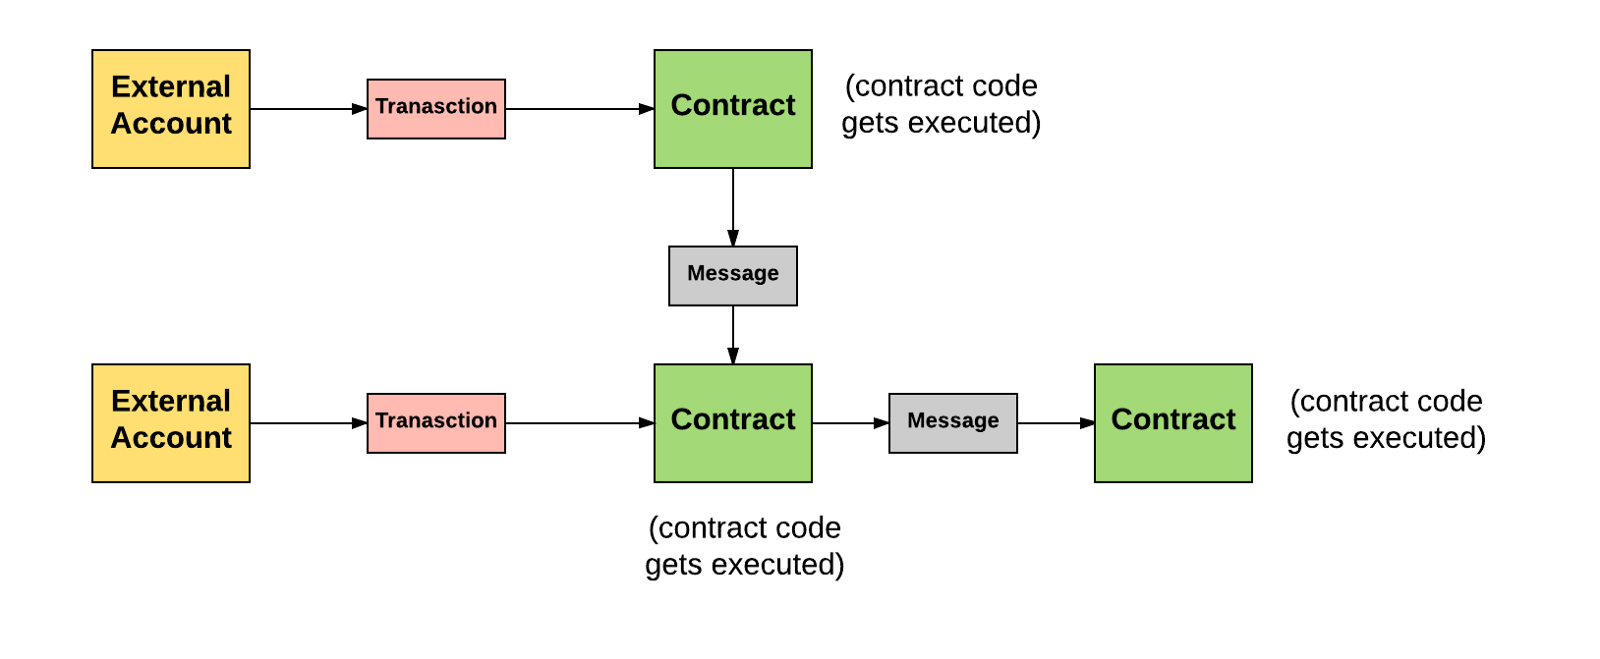
\includegraphics[width=.9\textwidth]{Ethereum/accounts}
		%
		\caption{Esempio di interazione tra accounts}
		%
		\label{fig:esempio di interazione tra accounts}
		%
	\end{figure}
	%
\end{center}
All'interno di Ethereum quindi gli account possono interagire tra di loro tramite messaggi oppure tramite transazioni.
%
\section{Messaggi e Transazioni}
%
\subsection{Transazioni}
%
Il termine \emph{transazione}, in Ethereum, viene utilizzato per riferirsi all'insieme di dati firmati che contengono un messaggio da inviare da un account posseduto dall'esterno. Le transazioni contengono:
\begin{enumerate}
	\item il destinatario del messaggio;
	\item una firma che identifica il mittente;
	\item l'ammontare di ether da trasferire al destinatario;
	\item un campo dati opzionale;
	\item un valore chiamato \emph{STARTGAS}: rappresenta il massimo numero di steps computazionali che l'esecuzione della transazione può impiegare;
	\item un valore chiamato \emph{GASPRICE}:  rappresenta la commissione che il mittente paga per lo step computazionale;
	\item v, r, s: usati per generare la firma che identifica il mittente della transazione.
\end{enumerate}
%
I campi (1.), (2.), (3.) sono campi standard previsti da qualsiasi criptovaluta. Il campo dati (4.) non ha una struttuda di default, potrebbe contenere un messaggio arbitrario oppure il codice per creare un contratto. Infatti la virtual machine di Ethereum ha un codice operativo con cui un contratto può accedere ai dati. Ad esempio, se un contratto sta funzionando come un servizio di gestione di ricette mediche basato su blockchain, potrebbe interpretare i campi che gli vengono passati come i campi della ricetta relativa in modo tale da poterli salvare correttamente nello storage. \\
I campi STARTGAS e GASPRICE sono essenziali per il modello di servizio anti-denial di Ethereum. Infatti al fine di prevenire loop infiniti, accidentali o malevoli che siano, o evitare spreco computazione di codice, ad ogni transazione è richiesto di impostare un limite per l'uso degli step computazionali di codice di esecuzione. L'unita fondamentale di computazione è il \emph{gas}. Solitamente uno step computazionale costa 1 gas ma potrebbe anche costa di più in quanto dipende dal livello di complessità computazionale delle operazioni o dalla quantità di dati che deve essere conservata come parte dello stato.\\
Infine, anche in Ethereum è presente una commissione (di gas) per ogni byte della transazione. Questa commissione ha uno scopo ben preciso, ovvero quello di obbligare un qualsiasi aggressore della rete a pagare proporzionalmente per ogni risorsa che essi vogliano consumare andando quindi ad includere la computazione, la larghezza di banda e lo storage.
%
\subsection{Messaggi}
%
I contratti hanno l'abilità di inviare "messaggi" ad altri contratti. I messaggi sono oggetti virtuali che non vengono mai serializzati ed esistono solo nell'ambiente di esecuzione di Ethereum (questi messaggi interni non sono quindi mai pubblicati sulla blockchain). Un messaggio è composto dai seguenti campi:
\begin{enumerate}
	\item il mittente del messaggio (implicito);
	\item il destinatario del messaggio;
	\item l'ammontare di ether da inviare attraverso il messaggio;
	\item un campo dati;
	\item un valore STARTGAS.
\end{enumerate}%
Un messaggio quindi è simile ad una transazione, eccetto che esso viene prodotto da un contratto e non da un attore esterno. Un messaggio viene prodotto quando un contratto che sta eseguendo il codice effetta una \emph{call}, che produce ed esegue appunto un messaggio. Come succede in una transazione, un messaggio comporta che l'account del destinatario esegua il proprio codice. In definitiva i contratti possono avere relazioni con altri contratti così come avviene con degli attori esterni e questo permette di avere un alto grado di libertà nella costruzione di applicazioni complesse. \\
In questo ambiente, la quantità di gas necessaria ad una transazione o ad un contratto, si applica alla totalità del gas consumato da quella transazione e da tutte le subesecuzioni. Ad esempio:
\begin{enumerate}
	\item un attore esterno A trasmette una transazione a B con 1000 gas;
	\item B consuma 600 gas prima di inviare il messaggio a C;
	\item C consuma internamente 300 gas prima di ritornare;
\end{enumerate}%
Dopo questi step B può spendere solo altri 100 gas prima di rimanere a corto di gas.
%
\section{Funzione Transazione di Stato}
%
Ethereum, quindi, si presenta come una macchina a stati basata sulle transazioni. Infatti quando una transazione viene eseguita all'interno della blockchain, la transizione verso uno stato finale rappresenta, in qualsiasi momento, lo stato attuale di Ethereum. Ad esempio nella seguente figura possiamo osservare la transizione da uno stato "State" ad uno stato "State'":
\begin{center}
	%
	\begin{figure}[h!]
		%
		\centering
		%
		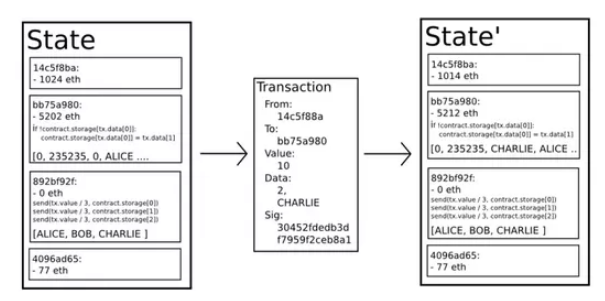
\includegraphics[width=.9\textwidth]{Ethereum/state}
		%
		\caption{Esempio di transizione di stato}
		%
		\label{fig:esempio di transazione di stato}
		%
	\end{figure}
	%
\end{center}
La funzione di transizione di stato di Ethereum può essere descritta, ad alto livello, nel seguente modo:
\begin{enumerate}
	\item controlla se la transazione è ben impostata (possiede il giusto numero di valori), se la firma è valida e il nonce corrisponde a quello dell'account del mittente. In caso contrario si verifica un abort;
	\item calcola la commissione di transazione come $STARTGAS*GASPRICE$ e determina l'indirizzo del mittente dalla firma. Sottrae poi la commissione dal bilancio dell'account del mittente e incremente il nonce del mittente. In caso in cui il bilancio da spendere sia insufficiente si verifica un abort;
	\item inizializza $GAS = STARGAS$ e toglie una certa quantità di gas per byte per pagare i byte della transazione;
	\item trasferisce il valore della transazione dall'account del mittente all'account del destinatario. Se l'account del destinatario non esiste ancora, lo crea. Se invece l'account destinatario è un contratto, esegue il codice del contratto per il completamento o fino all'esaurimento del gas;
	\item se il trasferimento del valore fallisce perchè il mittente non ha abbastanza soldi, il codice dell'esecuzione esaurisce il gas e ripristina tutti i cambiamenti di stato tranne che per il pagamento della commisione e aggiunge le stesse commissioni sul conto del minatore;
	\item se l'esecuzione termina correttamente, risarcisce al mittente le commissioni per il gas rimanente ed invia le commissioni pagate per il gas e consumante al miner.
\end{enumerate}%
\subsection{Esecuzione del Codice}
%
Il codice nei contratti Ethereum è scritto in un linguaggio di basso livello denominato \emph{codice virtual machine Ethereum} oppure \emph{codice EVM} che consiste in una serie di byte, dove ogni byte\footnote{in realtà il codice viene solo successivamente compilato in bytecode. Lo sviluppatore può servirsi di linguaggi di alto livello come Solidity o Serpent} rappresenta un'operazione eseguita all'interno dell'Ethereum Virtual Machine. \\ 
L'Ethereum Virtual Machine (EVM) è, quindi, l'ambiente di runtime per gli Smart Contract in Ethereum. L'ambiente risulta completamente sandboxato ed isolato il che significa che il codice in esecuzione al suo interno non ha accesso alla rete, al filesystem o ad altri processi. In generale, l'esecuzione del codice è un loop infinito che consiste nel realizzare ripetutamente l'operazione al contatore attuale del programma (che parte da 0) e incrementa il contatore di un'unità fino ad ottenere:
\begin{itemize}
	\item la fine del codice;
	\item un errore o STOP;
	\item viene rilevata l'istruzione RETURN.
\end{itemize}%
Le operazioni hanno accesso a tre tipi di spazio nel quale registrare i dati:
\begin{enumerate}
	\item Stack: un contenitore di tipo Last-In-First-Out (LIFO) nel quale i valori possono essere spinti;
	\item Memoria: un array di byte temporaneo (volatile) espandibile all'infinito;
	\item Storage: memoria non volatile mantenuta come parte dello stato e caratterizzata dall'essere di tipo chiave-valore.
\end{enumerate}%
La struttura dell'EVM è la seguente:
\begin{center}
	\begin{figure}[h!]
		%
		\centering
		%
		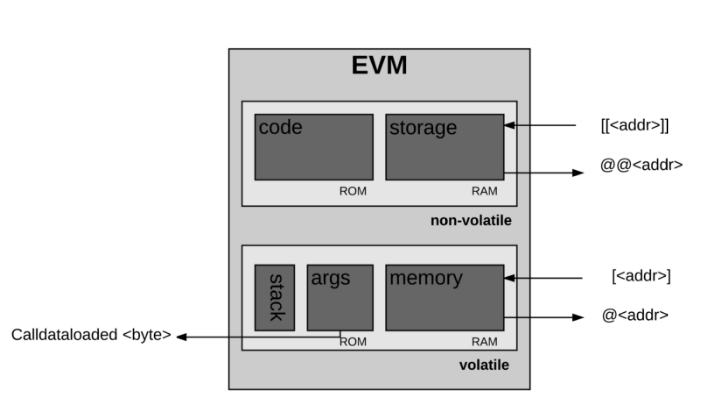
\includegraphics[width=.85\textwidth]{Ethereum/evm}
		%
		\caption{Schema dell'Ethereum Virtual Machine (EVM)}
		%
		\label{fig:schema dell'ethereum virtual machine}
		%
	\end{figure}
	%
\end{center}
Il modello di esecuzione formale del codice EVM risulta estremamente semplice. Infatti mentre la virtual machine di Ethereum funziona, tutto il suo stato computazionale può essere definito dall'insieme di dati (\emph{$stato_del_blocco$, transazione, messaggio, codice, memoria, stack, pc( i.e. program counter), gas}) dove $stato_del_blocco$ rappresenta lo stato globale che contiene tutti gli accounts e include i bilanci e lo storage. 
%
\section{Mining e Validazione}
%
Una volta validate, tutte le transazioni devono essere inserite in un blocco che deve essere anch'esso validato all'interno della rete. Un blocco (block header) in Ethereum si presenta nel seguente modo:
\begin{center}
	%
	\begin{figure}[h!]
		%
		\centering
		%
		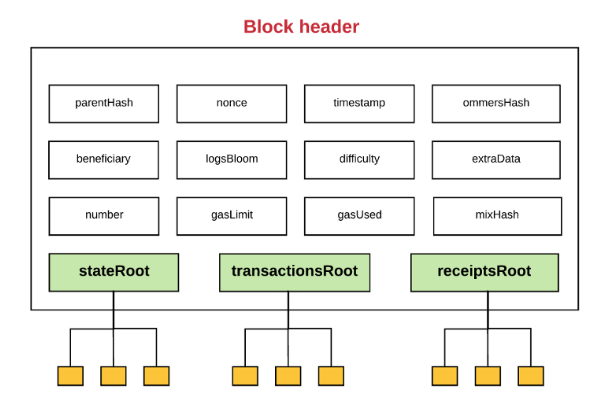
\includegraphics[width=.6\textwidth]{Ethereum/blockHeader}
		%
		\caption{Blocco in Ethereum}
		%
		\label{fig:blocco in Ethereum}
		%
	\end{figure}
	%
\end{center}
Per una descrizione dettagliata della struttura del block header si rimanda all'\autoref{cap:blockheader}. \\
L'algoritmo di validazione del blocco in Ethereum funziona nel seguente modo:
\begin{itemize}
	\item controlla se il precedente di riferimento essite ed è valido;
	\item controlla se la marca temporale del blocco è più grande di quella del blocco di riferimento precedente ed inferiore a 15 minuti nel futuro;
	\item controlla se il numero di blocco, la difficoltà del blocco, il transaction root, l'uncle root e il GASLIMIT sono validi;
	\item controlla se la proof-of-work sul blocco sia valida;
	\item sia $S[0]$ lo stato finale del blocco precedente;
	\item sia data la lista TX delle transazioni del blocco, con \emph{n} transazioni. Per tutti $i$ in $0..n-1$ sia $S[i+1]$ il risultato dell'applicazione della funzione transazione di stato sulla $TX[i]$ (ovvero ottengo il nuovo stato finale).\\ Viene restituito un errore in caso di superamento del GASLIMIT o in caso di errore dell'applicazione;
	\item sia lo stato finale $S[n]$ aggiungendo però la ricompensa per il blocco pagata al miner;
	\item l'algoritmo controlla che il root state del merkle tree sia uguale allo state root finale fornito nell'intestazione del blocco. Se i due valori corrispondono il blocco viene dichiarato valido. 
\end{itemize}%
Come in Bitcoin, anche in Ethereum la fase del mining passa attraverso la proof-of-work chiamata "Ethash" (conosciuta precedentemente come Dagger-Hashimoto)\cite{dh}. \\ L'algoritmo di valutazione, che a prima vista potrebbe sembrare inefficiente dato che registra l'intero stato di ogni blocco, risulta a livello di efficienza comparabile con quella di Bitcoin. Questo perchè lo stato viene registrato in una struttura ad albero e dopo ogni blocco solo una minima parte dell'albero necessita di essere cambiata. Quindi, in generale, tra due blocchi adiacenti la grande maggioranza dell'albero dovrà essere la stessa e quindi i dati possono essere registrati solo una volta e referenziati due volta tramite puntatori (ad es. gli hash degli alberi inferiori). Per raggiungere tutto questo Ethereum utilizza un tipo di albero conosciuto come \emph{Patricia Tree}\footnote{Permette ai nodi di essere non solo modificati con efficienza, ma anche inseriti e cancellati} , che consiste in una modifica ai Merkle Tree descritti in precedenza. Inoltre dato che tutta l'informazione sullo stato è una parte dell'ultimo blocco, non c'è bisogno di registrare tutta la storia della blockchain (ulteriore punto a favore rispetto alla blockchain di Bitcoin). 
%
 
%
% ------------------------------------------------------------------------ %
% !TEX encoding = UTF-8 Unicode
% !TEX TS-program = pdflatex
% !TEX root = ../Tesi.tex
% !TEX spellcheck = it-IT
% ------------------------------------------------------------------------ %
%
% ------------------------------------------------------------------------ %
% 	NOME CAPITOLO
% ------------------------------------------------------------------------ %
%
\chapter{Software Ethereum-based per Blockchain private: Quorum}
%
\label{cap:quorum}
%
% ------------------------------------------------------------------------ %
%
\section{Introduzione}
%
Come abbiamo scritto nei precedenti capitoli, gli Smart Contract si presentano come un libro mastro condiviso e replicato in ambiente Enterprise con la promessa di migliorare l'efficienza e diminuire i costi comparati con le altre soluzioni fornite da sistemi enterprise pre-esistenti\footnote{Ad esempio Zcash} basati sulla logica di business duplicata e su un protocollo del consenso basato sulla riconciliazione. Però gli attuali sistemi basati su smart contracts non sono capaci di fornire la privacy di dati essendo lo stato delle transazioni e degli smart contract esposti in chiaro nella rete. Questo lavoro di tesi concentra la sua attenzione su una blockchain che è stata costruita sulle specifiche di Ethereum e poi modificata per ottenere i requisiti di privatezza in ambiente enterprise, dove avviene lo scambio dati sensibili (come ad esempio i dati medici).\\
\emph{Quorum}\autocite{website:quorum} è un libro mastro distributo, privato, permissioned ed Ethereum-based che è stato sviluppato da J.P. Morgan per fornire all'industria dei servizi finanziari un'implementazione di Ethereum basata su permessi che possa supportare la privacy di contratti e transazioni. Quorum include quindi un fork minimo del client Ethereum (ovvero geth) facendo così leva sui traguardi tecnologici raggiunti dalla comunità degli sviluppatori di Ethereum.\footnote{ La libreria go-ethereum e i suoi file binari sono licenziati sotto la GNU Lesser General Public License v3.0} Le feature principali di Quorum, che corrispondono anche alle principali aggiunte rispetto alla blockchain pubblica Ethereum, sono:
\begin{enumerate}
	\item privatezza di contratti e transazioni. Quorum supporta transazioni e contratti privati attraverso la separazione tra stato pubblico e privato servendosi di \emph{constellation} uno strumento per lo scambio di messaggi criptati peer-to-peer per lo scambio diretto privati tra i partecipanti della rete;
	\item meccanismo di consenso basato sul voto multiplo. Essendo quorum una blockchain privata i partecipanti sono noti e non è strettamente necessario utilizzare la proof-of-work;
	\item gestione dei permessi sia a livello di rete che a livello di singolo peer. Il permissioning viene realizzato utilizzando la logica degli smart contracts;
	\item performance maggiori rispetto alla sua controparte pubblica.
\end{enumerate}%
%
\begin{figure}[H]
	%
	\centering
	%
	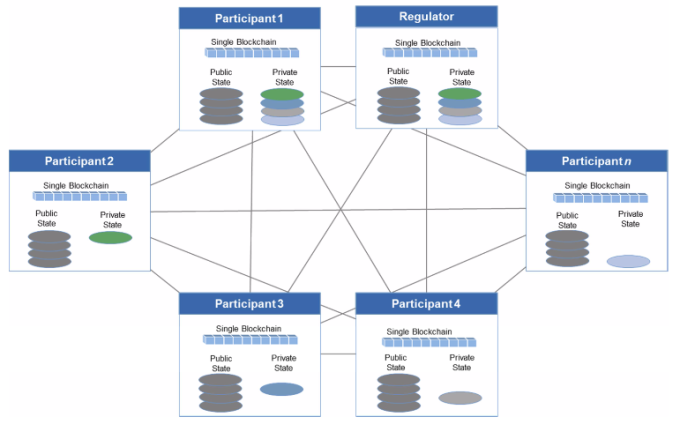
\includegraphics[width=.9\textwidth]{Quorum/quorum}
	%
	\caption{Diagramma di Quorum}
	%
	\label{fig:diagramma di quorum}
	%
\end{figure}
%
Lo scopo principale degli sviluppatori è stato quello di riutilizzare per quanto possibile l'attuale tecnologia minimizzando i cambiamenti rispetto all'attuale versione di Ethereum sia per favorire i tempi di sviluppo e deploy delle applicazioni decentralizzate sia per minimizzare lo sforzo di mantenere sincronizzata la code-base comune di Ethereum presente in Quorum. Inoltre, anche se è stata pensata in prima istanza per implementare servizi finanziari in cui si vuole comunque mantenere una figura di tipo controllore all'interno della rete, è possibile utilizzare Quorum per ambiti esterni alla finanza in quanto mantiene tutte l'espressività a livello di codice della blockchain Ethereum.
%
\section{Architettura}
%
Attualmente Quorum include le seguenti componenti:
%
\begin{figure}[H]
	%
	\centering
	%
	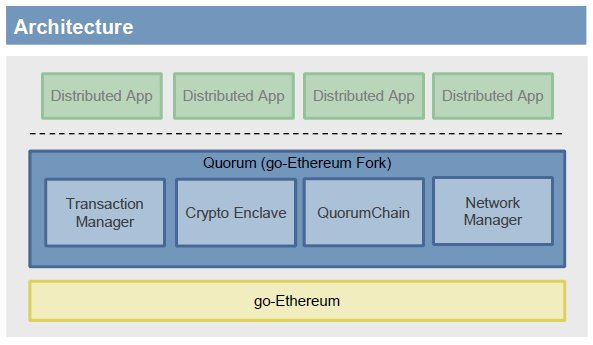
\includegraphics[width=.9\textwidth]{Quorum/comp}
	%
	\caption{Componenti di Quorum}
	%
	\label{fig:componenti di quorum}
	%
\end{figure}
%
L'essenza di Quorum è quella di utilizzare la crittografia al fine di prevenire l'accesso ai dati sensibili a chiunque, eccetto per gli utenti coinvolti. Questa soluzione è stata realizzata utilizzando una singola blockchain condivisa e combinando l'architettura software degli smart contract (che fornisce la segmentazione dei dati privati) e le modifiche al client Ethereum (che include le modifiche al processo di proposta e validazione dei blocchi). Le sue componenti principali sono le seguenti:
%
\paragraph{Quorum Node}
%
Un nodo Quorum corrisponde al client geth modificato. Rispetto alla sua controparte pubblica contiene le seguenti modifiche:
\begin{enumerate}
	\item l'algoritmo di consenso basato sulla proof-of-work è stato rimpiazzato da un meccanismo di tipo vote-based (più adatto alle blockchain private) denominato \emph{QuorumChain}. Quorum attualmente offre anche delle alternative rispetto a QuorumChain stesso:
	      \begin{itemize}
	      	\item \emph{Raft-based Consensus}: un modello di consenso per tempi di blocco maggiori, immutabilità delle transazioni e creazioni di blocchi on-demand.
	      	\item \emph{Istanbul BFT}: un algoritmo di consenso basato sul "Practical Byzantine Fault Tolerance" (PBFT).\cite{pbft}
	      \end{itemize}%
	\item il layer P2P è stato modificato al fine di permettere connessioni solo da/verso nodi autorizzati;
	\item sia la logica di generazione del blocco che la logica di validazione del blocco sono state modificate per sostituire il "Global state root" nel block header di Ethereum con il "Global public state root". Inoltre la logica di validazione del blocco è stata ulteriormente modificata per supportare le transazioni private;
	\item il Patricia tree è stato diviso in: public state tree e private state tree;
	\item la creazione delle transazioni è stata modificata per permettere che i dati della transazione vengano sostituiti con l'hash crittografico al fine di preservare la privatezza del dato quando richiesto;
	\item Il prezzo del Gas è stato rimosso (anche se il concetto di gas rimane presente all'interno della blockchain).
\end{enumerate}%
%
\paragraph{Constellation}
%
Constellation è un sistema general purpose per trasmettere informazioni in modo sicuro. Può essere paragonato ad una rete di MTA (Message Transfer Agents) dove i messaggi sono criptati tramite il software \enquote*{\gls{pgp}}. Non è un modulo pensato specificatamente per le blockchain ma è utilizzabile ogni volta che si vuole scambiare messaggi \enquote*{sigillati} individualmente all'interno di una rete di partecipanti. Questo componente è composto da due sotto componenti: il nodo Constellation (che viene utilizzato nell'implementazione standard del \emph{PrivateTransactionManager}) ed Enclave.%
\subparagraph{Il Transaction Manager.} È responsabile per la privacy delle transazioni. Esso infatti conserva e permette l'accesso ai dati criptati delle transazioni, lo scambio di payload criptati con i transaction manager degli altri partecipanti e, al tempo stesso, non ha accesso ad alcuna chiave privata sensibile. Utilizza Enclave per le funzionalità crittografiche. Ogni Quorum node possiede il suo Transaction Manager che dialoga con le sue controparti distribuite sugli altri nodi.%
\subparagraph{Enclave.} Abbiamo visto come i protocolli di ledger distribuiti facciano tipicamente uso di tecniche crittografiche per l'autenticità delle transazioni, l'autenticazione dei partecipanti e la conservazione storica dei dati (attraverso una catena di hash crittografici dei dati). Al fine di ottenere una separazione di compiti e al tempo stesso di garantire un miglioramento delle performanze attraverso la parallelizzazione delle operazioni che riguardano la crittografia, la maggior parte del lavoro crittografico inclusa la generazione di chiavi simmetriche e la cifratura/decifratura dei dati è delegata appunto ad Enclave. \\ Questo componente lavora quindi insieme al transaction manager per rafforzare la privacy attraverso la gestione della cifratura/decifratura in modo isolato. Esso quindi si comporta a tutti gli effetti come un \enquote*{Hardware Security Module} (HSM) isolato da tutti gli altri componenti.
%
\paragraph{Il Network Manager} si occupa del controllo degli accessi alla rete, permettendo quindi la creazione di una rete permissioned. %
%
\section{Transazioni}
%
Un'altra delle feature chiave di Quorum, come abbiamo detto, è la privatezza delle transazioni. Quorum infatti introduce la nozione di \emph{transazione privata} contrapposta alla classica \emph{transazione pubblica}. Questo però non vuol dire che gli sviluppatori di quorum hanno introdotto un nuovo tipo di transazione stravolgendo quindi il modello di Ethereum, bensì hanno esteso l'Ethereum Transaction Model nel seguente modo:
\begin{itemize}
	\item viene aggiunto un parametro opzione \emph{privateFor}\footnote{privateFor è un array di chiavi pubbliche} che, quando specificato, contraddistingue una transazione come privata e i nodi della blockchain la tratteranno di conseguenza;
	\item viene aggiunto un nuovo metodo al Transaction Type, denominato \emph{isPrivate}, necessario per identificare le nuove transazioni private.
\end{itemize}%
\paragraph{Transazioni pubbliche}%
Le transazioni pubbliche sono quelle transazioni in cui il payload è visibile a tutti i partecipanti della rete Quorum (hanno la stessa visibilità delle transazioni in Ethereum). Questo tipo di transazione viene eseguito nel modo standard di Ethereum ovvero se una transazione pubblica viene inviata ad un account che possiede il codice di un contratto, ogni partecipante eseguirà lo stesso codice e il loro stateDb verrà aggiornato di conseguenza. Il valore $V$ della firma della transazione viene settato dal nodo Quorum a $27 o 28$.
%
\paragraph{Transazioni private}%
Le transazioni private sono quelle transazioni in cui il payload è visibile solamente ai partecipanti della rete le cui chiavi pubbliche sono specificate nel parametro privateFor della transazione. Quando il nodo di Quorum incontra una transazione con un parametro privateFor non nullo, setta il valore $V$ della firma della transazione a $37 o 38$. Le transazioni private non sono eseguite nella modalità standard di Ethereum. Infatti prima che il nodo di Quorum del mittente propaghi la transazione al resto della rete, rimpiazza il payload originale della transazione con un hash del payload crittografato che riceve dal modulo Constellation. I partecipanti che fanno parte della transazione potranno rimpiazzare l'hash con il payload attuale attraverso la loro istanza di Constellation, chiamare l'EVM per l'esecuzione ed il loro stateDb sarà aggiornato di conseguenza. Invece i partecipanti che non fanno parte della transazione potranno leggere solamente l'hash e non eseguiranno la transazione (la transazione sarà a tutti gli effetti saltata da loro). Quindi questi due set di partecipanti termineranno con differenti stateDb e non potranno raggiungere il consenso perciò Quorum, al fine di supportare questa "biforcazione" dello stato del contratto immagazzina lo stato del contratto pubblico in un \emph{Public State trie} sincronizzato globalmente mentre immagazzina lo stato dei contratti privati in un \emph{Private state trie} non sincronizzato globalmente. Inoltre un contratto privato può essere creato solo attraverso una transazione privata.\\
Per una descrizione del flusso di una transazione privata all'interno di Quorum, si rimanda all'\autoref{cap:transaction}.%
\section{Consenso in Quorum}
%
Quorum\footnote{Nella sua versione studiata 1.5} supporta il meccanismo di consenso denominato \emph{QuorumChain}, un algoritmo a tempo a maggioranza di voto che utilizza:
\begin{enumerate}
	\item uno smart contract per governare il consenso e gestire chi può partecipare al consenso;
	\item transazioni Ethereum per propagare i voti attraverso la rete;
	\item validazione della firma di Ethereum per validare le firme ricevute dai nodi \emph{maker} e \emph{voter}.
\end{enumerate}%
Quorum utilizza nel meccanismo di consenso una divisione di ruoli tra i nodi. Infatti all'interno della rete possono esistere nodi con il ruolo di \emph{Voter} il quale permette loro di votare quale blocco dovrebbe essere la testa canonica ad una particolare altezza. Il blocco più recente con la maggioranza dei voti viene considerato la testa canonica di una catena ed un blocco viene considerato valido se e solo se ha ricevuto un numero minimo di voti dai Voters (supera la soglia minima). \\ 
La creazione dei blocchi invece è consentita solo ai nodi a cui è stato dato il ruolo di \emph{Maker}. Un nodo con questo ruolo infatti può creare un blocco e firmarlo settando la sua firma nel campo \emph{extraData} del blocco. All'atto dell'importazione del blocco come parte della procedura di Block Header Validation, i nodi verificano che il blocco sia stato firmato da uno dei nodi con il ruolo maker andando a cercare l'indirizzo di chi ha firmato il blocco nella lista dei makers validi contenuta nel \emph{Voting contract}. \\
Un nodo può anche non ricevere un ruolo oppure riceverli entrambi.%
\subsection{Voting Smart Contract}
%
Quorumchain è implementata nel contratto \emph{Blockvoting} che è settato all'indirizzo $0x0000000000000000000000000000000000000020$ all'interno del Genesis Block\footnote{Il primo blocco della blockchain, contiene i parametri relativi all'inception della blockchain}. All'interno del client Quorum sono hard-codati:
\begin{itemize}
	\item quell'indirizzo;
	\item il bytecode pre-compilato per il contratto BlockVoting e il suo ABI\footnote{Application Binary Interface} associato.
\end{itemize}
Nel caso in cui le regole del consenso all'interno del contratto BlockVoting dovessero essere aggiornate allora il nuovo codice dovrà essere compilato ed il client Quorum dovrà essere aggiornato per riflettere il nuovo codice. Tramite il contratto possono essere aggiunti o rimossi sia i nodi Voters che i nodi Makers e può essere configurato il numero minimo di voti (soglia) prima che un blocco venga selezionato come vincitore. Infine, come parte della validazione del blocco, il contratto deve determinare l'ultimo blocco che soddisfa il numero richiesto di voti (l'altezza canonica della catena) sul quale il blocco proposto si dovrà agganciare (il genitore del blocco proposto). Nel contratto sono inoltre registrati gli indirizzi dei nodi makers e voters. In particolare deve esserci almeno un nodo maker configurato nel contratto. In realtà sia l'insieme iniziale dei voti maker che dei voters è preconfigurato nel genesis block tramite il file di configurazione \emph{genesis.json}, tuttavia una volta creata la rete i nodi maker possono aggiungere o rimuovere altri nodi maker inviando una transazione con la chiamata appropriata alla funzione contenuta nel contratto così come i nodi voters possono fare la stessa cosa verso altri nodi voters. %
\subsection{Observer node}%
Classe di nodi che non riceve ne il ruolo di maker ne quello di voter. Quindi non potranno prendere parte alla creazione di blocchi e alla votazione degli stessi ma bensì riceverà e validerà semplicemente i vari blocchi della rete.%
\subsection{Creazione e Votazione del blocco}%
Abbiamo visto come all'interno di una rete Quorum possano esistere più voti makers tuttavia, al fine di ridurre la probabilità per due o più maker di creare un blocco nello stesso momento, ogni maker genera un timeout che deve rispettare prima di poter creare un nuovo blocco. Il primo nodo maker ad uscire dal proprio timeout potrà creare il blocco e, una volta creato, genererà un nuovo timeout per se stesso e così via. Una volta che un nodo maker inizia il processo di creazione di un blocco, gli altri nodi maker resetteranno il proprio timeout corrente, generandone quindi uno nuovo e aspetteranno la sua fine prima di provare a creare un nuovo blocco. \\
La durata del timeout cade casualmente tra un valore minimo e un valore massimo espressi in secondi che sono definiti nella \emph{Blockmaker strategy} e può essere settato tramite la cli\footnote{Command Line Interface} flag \emph{--minblocktime} e \emph{--maxblocktime}. Saranno invece usati i default in caso in cui questi valori non saranno settati esplicitamente. \\
Dopo che un blocco è stato importato con successo come testa della catena, un nuovo blocco in attesa viene preparato sopra quel blocco. A questo punto tutte le transazioni processabili sono selezionate e applicate allo stato in sospeso nel nuovo blocco. Se il nodo è configurato con il ruolo Maker e gli viene ordinato di creare un blocco, prima convaliderà che l'hash del blocco genitore sia un hash canonico valido (ultimo blocco con numero di voti richiesto). Se questo blocco differisce dall'attuale testa locale, la creazione del blocco fallisce. Se invece il blocco è stato costruito sopra il blocco corretto, il nuovo blocco viene inserito nella catena di blocchi e propagato verso gli altri nodi. Durante questo processo, al fine di evitare il problema del \emph{Chain halting} che può essere causato della limitata disponibilità dei nodi online, il nodo Maker invierà voti (se è configurato per essere anche un Voters) per il blocco principale al fine di soddisfare la soglia e consentire alla catena di progredire. Questo ha naturalmente implicazioni di controllo e dovrebbe essere gestito assicurandosi che i nodi dei voters soddisfino i loro obblighi verso la rete rimanendo disponibili.\\
La fase di voto invece deve avvenire entro un periodo preciso la cui durata è legata alla durata della creazione del blocco appena descritta. Dopo aver validato con successo un blocco, i voters trasmetteranno un voto per blocco chiamando il contratto BlockVoting. Nel caso in cui due nodi maker escano contemporaneamente dal loro timeout e creino entrambi un blocco, i nodi voters voteranno su entrambi i blocchi, ma quello con più voti alla fine della finestra di votazione sarà quello selezionato per la testa canonica della catena. Una descrizione schematica del processo di creazione, validazione e consenso in Quorum è contenuto nell'\autoref{cap:conseus}. La struttura di un blocco Quorum includerà quindi:
\begin{enumerate}
	\item \emph{Global Transaction Hash}: l'hash di tutte le transazioni (pubbliche e private) presenti in un blocco;
	\item \emph{Public State root hash}: la controparte Quorum di quello che in Ethereum si chiama Global State root hash;
	\item firma del blocco Maker nel campo \emph{extraData}.
\end{enumerate}%
\section{Sicurezza in Quorum}%
Quorum è una blockchain di tipo permissioned ovvero è possibile controllare quale nodo può connettersi ad un dato nodo e anche quali nodi un dato nodo può chiamare. Al momento della scrittura di questo lavoro di tesi, Quorum gestisce i permessi a livello di nodo individuale tramite la cli flag \emph{--permissioned} all'atto dell'avvio del nodo. Se questa flag viene settata il nodo cerca un file chiamato $<data-dir>/permissioned-nodes.json$ che contiene la whitelist dei nodi a cui questo nodo può connettersi e da cui può accettare connessioni. Quindi, con il flag abilitato solo i nodi che sono elencati nel file di configurazione json diventano parte di una rete, ma se il file dovesse essere vuoto a quel punto il nodo non potrà connettersi a nessun nodo ne accettare nessuna connessione in ingresso. Il file $permissioned-nodes.json$ ha una struttura precisa:
\begin{lstlisting}[language=json, firstnumber = 1]
{
	[ 
		"enode://remoteky1@ip1:port1",
		"enode://remoteky1@ip2:port2",
		"enode://remoteky1@ip3:port3", 
	]
}
\end{lstlisting}%
Ogni nodo avrà la sua versione di questo file.%
\subsection{Enclave}%
Enclave critta i payload che riceve dal Transaction Manager usando\footnote{Sono primitive contenute nella "Networking and Cryptography library" (NACL)} \emph{xsalsa20poly1305}\cite{nacl} (payload container) e  \emph{curve25519xsalsa20poly1305}\cite{nacl} (recipient box). Ogni crittografia del payload produce un payload container così come $N$ Recipent box dove $N$ è il numero dei destinatari specificato nel parametro "privateFor" della transazione. In particolare:
\begin{enumerate}
	\item il payload container contiene il payload crittato con la chiave simmetrica (\gls{simmetrica}) e un nonce casuale;
	\item il recipient box è la master key per il payload container crittato con la chiave pubblica di un destinatario utilizzando un nonce casuale (che corrisponde, in modo semplificato, al funzionamento di PGP ma usando le primitive crittografiche in NaCl);
\end{enumerate}
In questa versione di Quorum la whitelist delle chiavi pubbliche viene definita manualmente e non viene eseguita la rotazione automatica delle chiavi. Questa funzionalità verrà inserita nelle successive versioni. Inoltre risulta anche mancante un sistema di PKI essendo le chiavi generate casualmente e manualmente aggiunte alla whitelist (tutto questo viene effettuato e/o gestito da un operatore). \\
L'algoritmo per gestire le chiavi private è il seguente:
\begin{enumerate}
	\item Data una password P;
	\item Generato nonce casuale \emph{Argon2i};
	\item Generato nonce casuale \emph{NaCl secretbox};
	\item Eseguito lo stretch di P utilizzando \emph{Argon2i} (e \emph{Argon2i nonce}) in una \emph{master key} (MK) di 32-byte;
	\item Crittare la chiave privata nella secretbox usando \emph{secretbox nonce} e \emph{Argon2i-stretched MK}.
\end{enumerate} 
%
% ------------------------------------------------------------------------ %
% !TEX encoding = UTF-8 Unicode
% !TEX TS-program = pdflatex
% !TEX root = ../Tesi.tex
% !TEX spellcheck = it-IT
% ------------------------------------------------------------------------ %
%
% ------------------------------------------------------------------------ %
% 	NOME CAPITOLO
% ------------------------------------------------------------------------ %
%
\chapter{Strumenti di sviluppo}
%
\label{cap:strumenti}
%
% ------------------------------------------------------------------------ %
%
\section{Introduzione}
%
L'applicazione che si vuole implementare è costituita da tre tipologie di entità: le prime corrispondo agli account dei \emph{medici} che hanno il compito di creare e rilasciare le ricette mediche bianche dematerializzate ai pazienti che le richiedono; le seconde sono i \emph{farmacisti} che hanno il compito di accertarsi che la ricetta dematerializzata non sia stata manomessa per procedere all'erogazione dei farmaci contenuti nella ricetta stessa; le terze sono gli account che, in questa implementazione, avranno il ruolo di \emph{amministratore} (admin) con la possibilità di associare un determinato ruolo (medico o farmacista) agli account esistenti.\\
Questo tipo di sistema può essere realizzato utilizzando come infrastruttura una blockchain privata: questa catena infatti contiene un insieme di transazioni attestanti ogni ricetta emessa dai medici e garantisce l'immutabilità del contenuto delle ricette stesse, permettendo i controlli di integrità sui contenuti inseriti. Inoltre la blockchain viene condivisa da tutte le parti coinvolte che, previo permesso, all'atto dell'ingresso nella rete possono scaricare localmente la copia più aggiornata e da quel momento in poi possono interagire con essa con nuovi inserimenti. Questa tecnologia infine rende immediatamente disponibili ogni inserimento di ricetta medica che viene trasmesso ad ogni nodo della rete. \\ 
Per una maggiore velocità nello sviluppo del prototipo applicativo, esso è stato pensato come un applicativo web. Generalmente, la struttura di una web application può essere schematizzata come nella seguente figura:
\begin{center}
	%
	\begin{figure}[H]
		%
		\centering
		%
		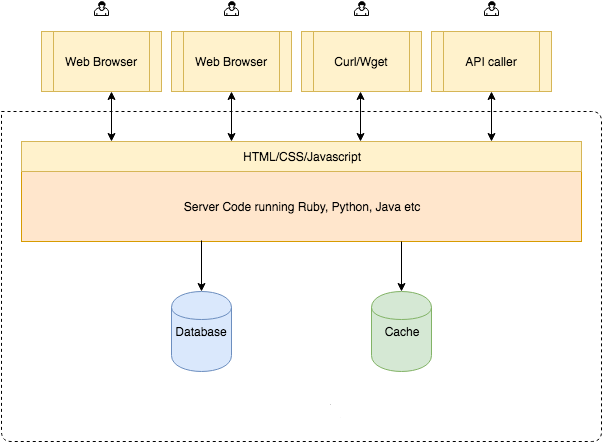
\includegraphics[width=.9\textwidth]{webapp}
		%
		\caption{Web application generica}
		%
		\label{fig:web application generica}
		%
	\end{figure}
	%
\end{center}
L'applicazione può essere ad esempio hostata su un servizio di hosting e tutti i client possono interagire con questa singola applicazione centrale. Un client può essere un browser oppure un'altra API che utilizza il servizio ecc. Quando il client effettua un richiesta al server quest ultimo prende in carico la richiesta, dialoga con il database e/o con la cache, legge/aggiorna/scrive il database\footnote{CRUD Model. Create, Read, Update, Delete} e serve il client. Questa tipologia di architettura è, al giorno d'oggi, una delle soluzioni tecniche più consolidate nell'ambito dello sviluppo del software. Però esistono anche determinate applicazioni dove sarebbe molto più utile se il database fosse ad esempio accessibile, in modo sicuro, da tutti senza dover dipendere da una terza parte. Questo è uno dei concetti chiave alla base di quelle che abbiamo definito precedentemente come \emph{Applicazioni decentralizzate} (Decentralized Application o Dapp). La struttura di una generica applicazione decentralizzata può essere invece schematizzata come segue:
\newline
%
\begin{center}
	%
	\begin{figure}[H]
		%
		\centering
		%
		\includegraphics[width=.9\textwidth]{dapp}
		%
		\caption{Decentralized application generica}
		%
		\label{fig:decentralized application generica}
		%
	\end{figure}
	%
\end{center}
Possiamo vedere come il client (nel nostro caso il browser) comunica con la propria istanza dell'applicazione. Non c'è alcun server centrale al quale i client si connettono. Ogni elemento in figura rappresenta una scelta tecnologica relativa allo sviluppo della dapp. In particolare:
\begin{enumerate}
	\item i contratti sono scritti in \emph{Solidity}, linguaggio per scrivere Smart contract Ethereum che girano sulla EVM;
	\item \emph{Truffle} è uno dei framework più utilizzati a disposizione dello sviluppatore per lo sviluppo e il testing in ambiente Ethereum;
	\item \emph{Web3.js} è una Api Javascript per i client Ethereum che permette di comunicare con il nodo locale attraverso Remote Procedure Calls (RPC);
	\item la blockchain alla base della Dapp sarà Quorum.
\end{enumerate}
%
\section{Solidity}
Solidità è un linguaggio di alto livello \enquote*{contract-oriented} per l'implementazione di Smart Contract su varie piattaforme di Blockchain. È stato sviluppato da Gavin Wood ed è stato influenzato da C++, Python e JavaScript. Questo linguaggio viene compilato in bytecode eseguibile nell'Ethereum Virtual Machine (EVM) e supporta l'ereditarietà, le librerie e i tipi complessi definiti dall'utente. \\ 
Con Solidity, gli sviluppatori sono in grado di scrivere applicazioni che implementano una logica di business autodefinita ed integrata nello Smart contract, fornendo una transazione non ripudiabile ed autorevole. Come specificato da Wood, il linguaggio è progettato attorno alla sintassi \emph{ECMAScript} per renderlo familiare agli sviluppatori web ma, a differenza di ECMAScript, ha tipizzazione statica e tipi di ritorno variadici. Rispetto ad altri linguaggi attuali che vengono eseguiti su EVM come Serpent e Mutan, Solidity presenta delle differenze importanti:
\begin{itemize}
	\item sono supportate variabili membro complesse per contratti, incluse mappature e strutture arbitrariamente gerarchiche;
	\item è supportata l'ereditarietà, inclusa l'ereditarietà multipla con la linearizzazione C3;
	\item introduce una ABI che facilita funzioni multiple con la type-safety\footnote{la "sicurezza di tipo" è il modo con cui un linguaggio di programmazione previene o avvisa gli errori di tipo};
	\item è supportato da un sistema di documentazione che specifica una descrizione, di tipo user-centric, delle ramificazioni di una chiamata del metodo nota come \enquote*{Natural Language Specification}.
\end{itemize}%
Solidity inoltre ha a disposizione un ulteriore strumento molto potente per gli sviluppatori, chiamato \emph{Remix}, che consiste in un IDE Browser-based con integrato il compilatore e l'ambiente di runtime di Solidity senza componenti server-side. Le sue caratteristiche principali sono:
\begin{enumerate}
	\item sviluppo di smart contracts grazie all'editor integrato solidity;
	\item debug dell'esecuzione di uno smart contract;
	\item accesso allo stato e alle proprietà di uno smart contract già stato deployato;
	\item debug di transazioni che hanno già effettuato il commit;
	\item analisi del codice per minimizzare l'errore e per forzare le best practises.
\end{enumerate}
%
\begin{figure}[H]
	%
	\centering
	%
	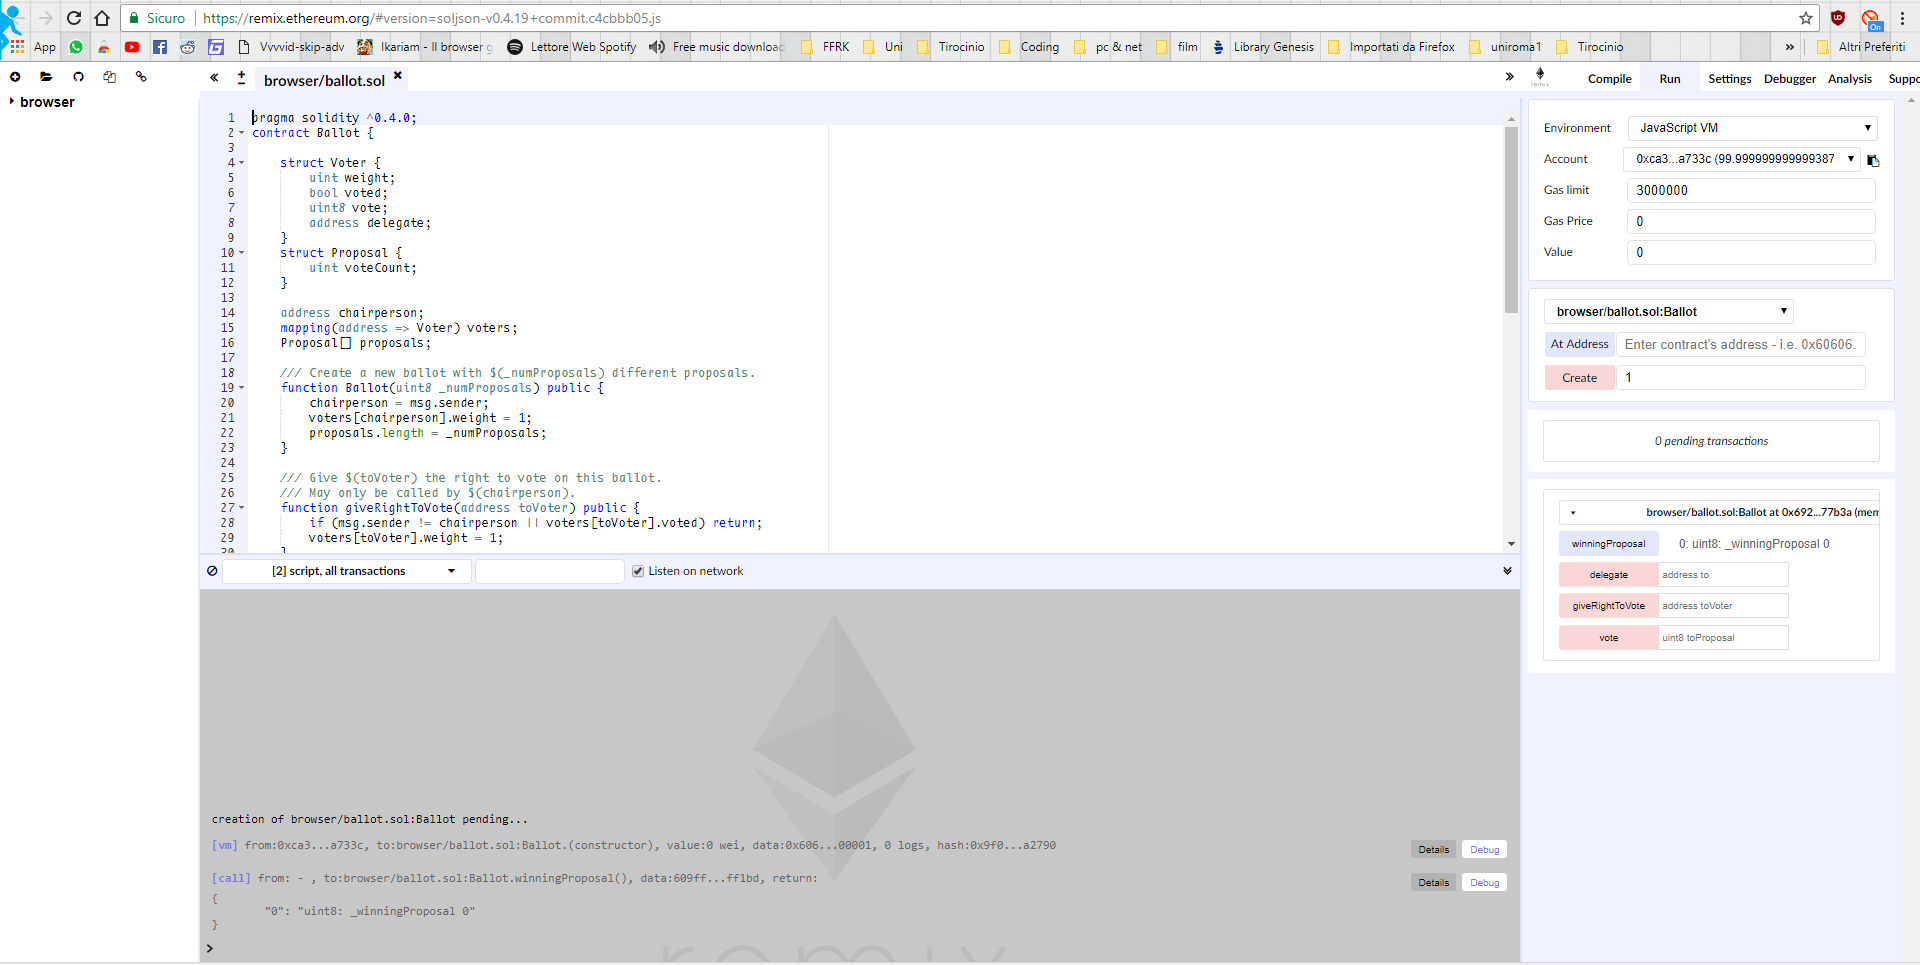
\includegraphics[width=.9\textwidth]{remix}
	%
	\caption{Remix IDE}
	%
	\label{fig:remix ide}
	%
\end{figure}
%
\section{Node.js \& Npm}%
\emph{Node.js} è un ambiente di run-time JavaScript, cross-platform e open-source per eseguire codice JavaScript lato server. Storicamente il linguaggio JavaScript è sempre stato principalmente usato come scripting lato client dove gli script erano integrati nelle pagine HTML per essere essere poi eseguiti dai motori JavaScript contenuti nei web browser degli utenti. Node.js permette al JavaScript di essere eseguito lato server per produrre pagine web dinamiche prima che esse vengano inviate al web browser dell'utente. Il modello di funzionamento di node è caratterizzato da un modello di I/O asincrono basato sugli eventi particolarmente adatto per le applicazioni web. La normale procedura di esecuzione di una applicazione server-side, scritta ad esempio in PHP, prevede lo scorrere di una serie di istruzioni che coinvolgono chiamate a servizi esterni come ad esempio query per un database, o l'accesso al filesystem per operazioni di lettura e scrittura. Tutti questi eventi sono bloccanti ovvero l'esecuzione dello script viene fermata finché non riceve una risposta dal componente esterno a cui l'ha richiesta. In tal modo il web server impiega la maggior parte del proprio tempo attendendo che i processi bloccati si completino, e questo porta ad una vistosa inefficienza nello sfruttamento delle risorse a disposizione. Tutto questo invece non succede in Node perchè, usando la programmazione asincrona, si elimina l'attesa e si eseguono le richieste successive, permettendo cosi un throughput e una scalabilità ottimizzate nelle web application. 
\subparagraph{Npm} è invece un gestore di pacchetti per il linguaggio JavaScript. In particolare è il gestore di pacchetti JavaScript predefinito nell'ambiente Node.js. Esso è composto da un client a riga di comando e da un database online di package pubblici (o moduli) denominato Npm registry. Un package è una directory che contiene uno o più file insieme ad un file chiamato package.json che contiene i dati relativi al pacchetto. Una web application che utilizza questa tecnologia per la gestione delle dipendenze in un progetto può contenere svariati pacchetti. Il vantaggio nell'usare un package manager risiede nella possibilità di aggiornare automaticamente tutte le dipendenze utilizzate evitando allo stesso tempo possibili "rotture" del codice causate da un aggiornamento manuale da parte dello sviluppatore. \\ 
Le tecnologie usate nello sviluppo dell'applicazione che si basano su Node.js sono:
\begin{itemize}
	\item Truffle framework;
	\item Express.js.
\end{itemize}
%
\subsection{Truffle Framework}
%
Truffle, attualmente, è il framework di sviluppo più popolare per applicazioni Ethereum based\footnote{Truffle supporta allo stesso modo la Blockchian Quorum essendo un fork di Ethereum}. Le feature che caratterizzano questo framework e che hanno portato alla sua scelta per lo sviluppo sono:
\begin{enumerate}
	\item \emph{Compilazione, linking, deployment e gestione dei binary degli smart contract integrata}. Il framework Truffle si occupa autonomamente della gestione degli artefatti dei contratti. Inoltre include il supporto per deploy custom, linking di librerie e applicazioni Ethereum complesse;
	\item \emph{Testing automatizzato dei contratti per un rapido sviluppo}. Truffle permette di scrivere test automatizzati sia in JavaScript che in Solidity per una maggiore rapidità di sviluppo;
	\item Permette di scrivere \emph{script di deploy custom} che riconoscono come l'applicazione possa cambiare nel tempo e che quindi permettono di avere uno sforzo di mantenimento minore;
	\item \emph{Gestione delle reti}. Truffle gestisce il deploy verso blockchain sia pubbliche che private. In questo modo lo sviluppatore non deve gestire manualmente gli artifatti di rete;
	\item Per utilizzare Truffle è necessario avere Node.js installato e questo permette di scaricare facilmente migliaia di dipendenze per gli Smart contracts via NPM;
	\item Truffle offre infine un ambiente ottimizzato nelle fasi di compilazione e test.
\end{enumerate}
Lo scheletro di un progetto Truffle è composto da quattro cartelle principali:
\begin{itemize}
	\item \emph{contracts/}: cartella dove sono contenuti i contratti Solidity.
	\item \emph{migrations/}: cartella dove sono contenuti gli scripts di migrazione.
	\item \emph{test/}: cartella dove sono contenuti i file per il test dell'applicazione e dei contratti.
	\item \emph{truffle.js}: file di configurazione di truffle.
\end{itemize}%
\subsection{Express.js}%
Express.js, o semplicemente Express, è un framework MVC per applicazioni web per Node.js, rilasciato come software libero ed open-source tramite MIT License ed è attualmente il framework server standard per Node.js. La filosofia di Express è quella di fornire un piccolo e robusto strumento per i server HTTP rendendolo la scelta preferita per le single page application, i siti web e le API. Come vedremo infatti, il compito principale di express all'interno del progetto sarà quello di gestire gli assett\footnote{I file statici come le viste} dell'applicazione e definire le rotte che saranno utilizzate per le richieste che arrivano dal client. Una rotta può essere una richiesta di tipo GET (semplice richiesta di file,passaggio di pochi parametri) e di tipo POST(passaggio di molti parametri con attivazione di logica lato server)
Nel nostro caso express ha in carico:
\begin{enumerate}
	\item gestione dei file statici dell'applicazione;
	\item la generazione del codice univoco NRE inserito nella ricetta dematerializzata ed utilizzato per la ricerca della ricetta stessa da parte dei farmacisti.
	\item la generazione server side del pdf della ricetta dematerializzata.
\end{enumerate}
La scelta di utilizzare di introdurre un elemento di tipo web server all'interno dell'architettura dell'applicazione è stata presa per motivi di sicurezza che saranno meglio spiegati durante la descrizione dell'implementazione dell'applicazione. 
%
\section{Web3.js} % 
Web3.js è una collezione di librerie scritte in JavaScript che permettono allo sviluppatore di interagire con un nodo locale o remoto di Ethereum/Quorum utilizzando una connessione HTTP o IPC. Web3 è necessaria affinche la dapp lavori con la blockchain in quanto fornisce lo strumento di comunicazione verso il nodo locale attraverso Remote Procedure Calls (RPC). In particolare, la libreria contiene un oggetto specifico per interagire con le blockchain Ethereum-based, l'oggetto \emph{web3.eth}. Per utilizzare la libreria, una volta importata nel progetto, si deve creare un'istanza di web3 andando a settare il provider per comunicare con il nodo locale:
\begin{lstlisting}[language=javascript]
	if (typeof web3 !== 'undefined') {
		web3 = new Web3(web3.currentProvider);
		} else {
		// set the provider you want from Web3.providers
		web3 = new Web3(new Web3.providers.HttpProvider("http://localhost:22000"));
	}
\end{lstlisting}%
A questo punto è possibile utilizzare le API dell'oggetto web3.
%
 
%
% ------------------------------------------------------------------------ %
% !TEX encoding = UTF-8 Unicode
% !TEX TS-program = pdflatex
% !TEX root = ../Tesi.tex
% !TEX spellcheck = it-IT
% ------------------------------------------------------------------------ %
%
% ------------------------------------------------------------------------ %
% 	NOME CAPITOLO
% ------------------------------------------------------------------------ %
%
\chapter{Configurazione dell'ambiente di sviluppo} % (fold)
%
\label{cap:configurazione}
%
\section{Introduzione}
Prima di procedere cn l'implementazione si è dovuti procedere a configurare l'intero ambiente di sviluppo locale relativo ai framework descritti nel capitolo precedente e al nodo locale della blockchain Quorum. Per lo sviluppo si è scelto di utilizzare un ambiente linux, precisamente Ubuntu 16.04 LTS. \\
La versione della blockchain Quorum utilizzata durante lo sviluppo di questa applicazione è stata la 1.5\footnote{Nel mese di ottobre Quorum è stata aggiornata ad una major version 1.8 per riallinearsi alla blockchain Ethereum (aggiornamento client geth in uso alla versione 1.7) e migliorare la propria gestione dei permessi e della privacy}, caratterizzata da una procedura di configurazione divisa in più step che permette di avere un ambiente Quorum completamente funzionale composto da sette nodi indipendenti. Gli sviluppatori di Quorum consigliano, per questa versione, di utilizzare \emph{Vagrant} e l'hypervisor di \emph{Virtualbox}.%
\section{Vagrant} 
Vagrant è un software open-source progettato per cotruire e mantenere ambienti di sviluppo software portabili, capace di utilizzare i maggiori hypervisor attualmente utilizzati come VirtualBox (scelta predefinita all'atto dell'installazione), Hyper-V, Docker, VMware e KVM. L'idea alla base di questo software risiede nel fatto che mantenere l'ambiente di configurazione diventa particolarmente difficoltoso con l'aumentare delle tecnologie utilizzate in uno specifico progetto. Vagrant semplifica i passi della gestione delle configurazioni software al fine di aumentare la produttività dello sviluppo. Vagrant è scritto in Ruby ma il suo ecosistema supporta quasi tutti i maggiori linguaggi. Il software si basa sul concetto di "box". Una box può essere paragonata ad una scatola contenente il sistema operativo, e tutto quello di cui abbiamo bisogno come i software di base ed ogni loro configurazione associata. Invece le impostazioni del software che regolano la creazione di una determinata box sono racchiuse in un file scritto in ruby denominato \enquote*{VagrantFile}. \\
Quindi, una volta scaricato ed installato sia VirtualBox che Vagrant, il passo successivo è stato quello di customizzare i file di configurazione di Vagrant utilizzati nello sviluppo. Per completezza, i file sono stati inseriti nell' \autoref{cap:codici} relativa ai codici utilizzati nel progetto, nella sezione ~\nameref{cap:vagrantConfig}, contiene:
\begin{enumerate}
	\item la box utilizzata. Nel nostro caso \emph{Ubuntu 16.04.3 LTS} (xenial);
	\item la direttiva che specifica l'esecuzione di un file script di configurazione immediatamente dopo la creazione della box (bootstrap.sh);
	\item il mapping delle porte TCP/UDP tra la macchina guest e la macchina host;
	\item la quantità di memoria allocata alla box.
\end{enumerate}
Il file realizzato per configurare la macchina dopo la sua creazione è denominato \emph{bootstrap.sh} e contiene tutte le direttive per installare tutte le dipendenze di Quorum per avere una blockchain completamente funzionante. La sua esecuzione avrà come risultato:
\begin{enumerate}
	\item l'aggiunta del repository ppa:ethereum/ethereum per avere l'accesso in download dei pacchetti Ethereum necessari in Quorum;
	\item l'installazione di Constellation ed Enclave;
	\item l'installazione di Golang, linguaggio di programmazione denominato "GO" scritto da Google. Il core di Quorum infatti è scritto in GO;
	\item la build dei file sorgenti di Quorum scaricati dal repository di Quorum;
\end{enumerate}
Il risultato di bootstrap.sh è un ambiente Quorum pronto per essere utilizzato. Una volta preparati i file, la procedura automatizzata di installazione e configurazione viene lanciata tramite il comando da shell: \emph{vagrant up}. Terminata la configurazione, è possibile accedere alla macchina (e quindi alla blockchain) tramite il comando da shell: \emph{vagrant ssh} che avrà il seguente output:
%
\begin{figure}[H]
	%
	\centering
	%
	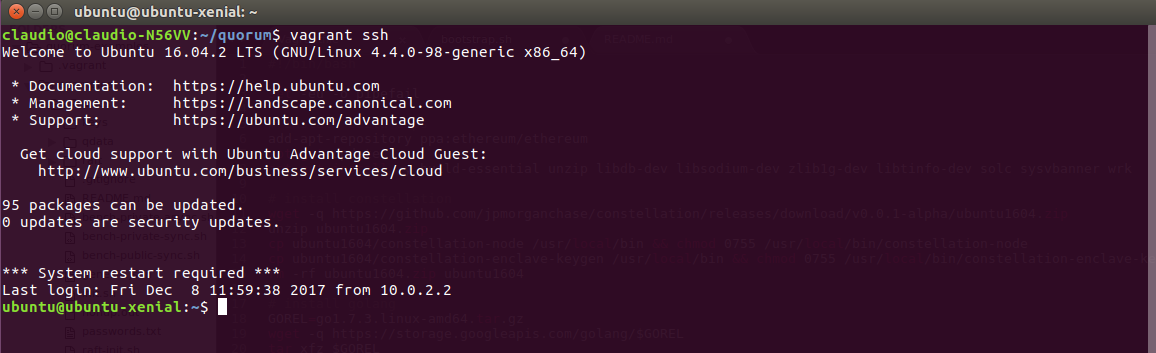
\includegraphics[width=.8\textwidth]{Implementazione/vagrantssh}
	%
	\caption{Terminale per interagire con la blockchain via ssh}
	%
	\label{fig:terminale per interagire con la blockchain}
	%
\end{figure}
%
\section{Quorum}
%
Una volta stabilita la connessione con la macchina virtuale contenente la blockchain, possiamo vedere come l'esecuzione del file bootstrap.sh descritto in precedenza, ha creato due cartelle nella home della macchina:
\begin{itemize}
	\item una cartella \emph{quorum} contenente tutti i file necessari al corretto funzionamento della blockchain;
	\item una cartella \emph{quorum-examples} contenente i file per gestire e personalizzare una istanza locale di Quorum composta da sette nodi indipendenti.
\end{itemize}
Nella cartella \enquote*{quorum-examples/7nodes} troviamo i file per interagire con la blockchain, come possiamo vedere nella seguente immagine:
%
\begin{figure}[H]
	%
	\centering
	%
	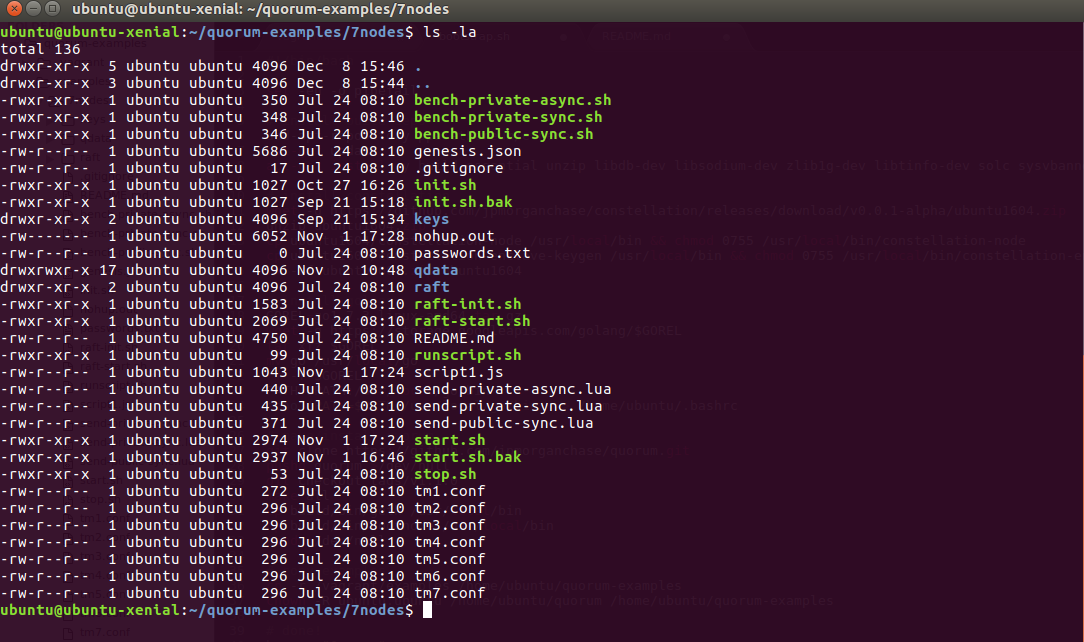
\includegraphics[width=.9\textwidth]{Implementazione/7nodes}
	%
	\caption{Struttura dei file della Blockchain Quorum}
	%
	\label{fig:file blockchain quorum}
	%
\end{figure}
%
In particolare, i file che ci interessano in questa fase di avvio sono:
\begin{enumerate}
	\item \emph{init.sh}. Script da terminale per inizializzare la blockchain. Pulisce le cartelle con i file temporanei locali della blockchain ed inizializza i 7 nodi della blockchain;
	\item \emph{start.sh}. Avvia la blockchain (può accettare ulteriori parametri di configurazione a livello di singolo nodo;
	\item \emph{stop.sh}. Termina tutti i processi della blockchain in modo sicuro.
\end{enumerate}
Questi file, in particolare init.sh e start.sh sono stati modificati per venire incontro alle esigenze dell'applicazione. Anche in questo caso, per l'intera struttura dei file, si rimanda all'\autoref{cap:codici} nella sezione ~\nameref{cap:quorumCode}.
\subsubsection{init.sh}
Il file init.sh è stato riorganizzato al fine di avere, all'avvio della blockchain, due account correttamente configurati sul nodo 1 (dove sarà deployato successivamente il contratto). Per configurare correttamente gli account è necessario:
\begin{enumerate}
	\item per ogni nodo corrispondente viene creata una cartella che andrà a contenere i \emph{keystore} associati ad ogni account e si copiano le informazioni relative alle chiavi pubbliche degli account in ognuna delle cartelle, ove necessario;
	\item si inizializzano i client geth (uno per nodo) tramite i file copiati, a seconda di come si vuole avviare la blockchain, e tramite l'utilizzo ulteriore del file \emph{genesis.json}.
\end{enumerate}
Nel caso invece si vogliano aggiungere ulteriori account, basterà generare tutte le informazioni e le chiavi per il nuovo account tramite Constellation e poi modificare il file init.sh (e lo start.sh di conseguenza).
\subsubsection{start.sh}
Il file start.sh contiente invece i comandi principali per lanciare correttamente l'esecuzione della blockchain. La sua esecuzione ha i seguenti risultati:
\begin{enumerate}
	\item la configurazione del bootnode della blockchain con le direttive a tutte le componenti (eth, web3, quorum ecc);
	\item l'avvio di un'instanza di Constellation per nodo;
	\item l'avvio del bootnode;
	\item l'avvio dei 7 nodi della blockchain. Per lo sviluppo è stata usata la seguente struttura di nodi:
	      \begin{itemize}
	      	\item sul nodo 1 vengono configurati due account, uno dei quali con ruolo voter;
	      	\item sul nodo 2 vengono configurati due account, uno con ruolo voter ed uno con voto maker;
	      	\item nodo 3 configurato senza account;
	      	\item sul nodo 4 viene configurato un nodo voter;
	      	\item i nodi 5,6 e 7 vengono configurati senza account.
	      \end{itemize}
\end{enumerate}
A questo punto la blockchain risulta correttamente configurata ed avviata. Gli account saranno poi associati agli attori dell'applicazione, come vedremo in seguito.
%
\section{Node, Truffle \& Express}
Una volta configurata la blockchain è necessario configurare l'ambiente Node. Per farlo, si devono eseguire i seguenti comandi: 
\begin{itemize}
	\item \textit{\textbf{sudo apt-get install nodejs}}: verrà installata sulla macchina locale l'ultima versione di Node.js\footnote{La versione utilizzata nello sviluppo è stata la v.6.11.1};
	\item \textit{\textbf{sudo apt-get install npm}}: verrà installato il package manager di Node.js.
\end{itemize}
A questo punto è possibile creare la cartella di progetto da dentro cui si andranno ad eseguire i seguenti comandi da terminale:
\begin{itemize}
	\item \textit{\textbf{npm init}}. Questo comando andrà a creare il file \emph{package.json} per l'applicazione, un descrittore json con le informazioni base del progetto e delle sue dipendenze. I campi inseriti sono:
	      \begin{itemize}
	      	\item \emph{name}: nome dell'applicazione;
	      	\item \emph{version}: versione dell'applicazione che, insieme al name, crea un identificatore univoco.
	      	\item \emph{description}: descrizione dell'applicazione
	      	\item \emph{scripts}: dizionario chiave-valore che elenca gli script da lanciare (valore) associati agli eventi del ciclo di vita del progetto (chiave);
	      	\item \emph{dependencies}: contiene le dipendenze necessarie a runtime. Nel nostro caso contiene tutte le librerie per utilizzare correttamente le funzionalità offerte dall'applicazione.
	      \end{itemize}
	\item \textit{\textbf{npm install -g truffle}}: installa globalmente la libreria Truffle;
	\item \textit{\textbf{npm install -g express}}: installa globalmente la libreria Express.
\end{itemize}
A questo punto l'utente ha configurato tutto il necessario e può eseguire il comando \textit{\textbf{truffle init}} che andrà ad inizializzare la cartella di progetto con lo scheletro di progetto di Truffle visto precedentemente. A questo punto, l'ultimo cambiamento da effettuare è la modifica del file truffle.js per farlo puntare verso la blockchain (nel nostro caso è stato scelto il nodo 1 precedentemente configurato), che sarà quindi il localhost sulla porta 22000 (già autorizzata a livello di permessi).
%
\section{Deploy di un contratto sulla blockchain}
%
Una volta configurato truffle per inviare i contratti sulla blockchain si dovrà effettuare quella che viene definita \emph{migrazione}. La migrazione viene realizzata tramite file JavaScript che automatizzano l'attività di deploy del contratto sul nodo di Quorum. Questi file sono scritti in modo tale da poter essere facilmente mantenuti e modificati a seconda di come cambiano le necessità del progetto rispetto al deploy su una particolare blockchain. Si possono avere più file di migrazione all'interno del progetto. \\
Il comando per eseguire la migrazione è \emph{truffle migrate}. Questo comando eseguirà tutti i file di migrazione inseriti nella cartella \emph{migrations/}. Nel caso in cui tutte le migrazioni sono state eseguite con successo, l'esecuzione di truffle migrate partirà dall'ultimo file eseguito, andando ad eseguire solo le nuove migrazioni create. La migrazione verrà eseguita verso il nodo della blockchain specificato nel file \emph{truffle.js}. Per usufruire delle features delle migrazioni di Truffle è necessario avere all'interno del progetto il contratto di migrazione\footnote{Viene configurato in maniera autonoma dal comando \emph{truffle init}} e deve essere deployato come primo contratto nell'ordine di migrazione. \\
Il file di migrazione verso la blockchain Quoruma utilizzato nell'applicazione è il seguente:
\newline	
\begin{lstlisting}[language=javascript,caption={Script di migrazione del contratto dell'applicazione},captionpos=b,frame=lines,basicstyle=\linespread{0.9}\small]
var Prescriptions = artifacts.require("./Prescriptions.sol");
module.exports = function(deployer) {
  deployer.deploy(Prescriptions, {privateFor: ["ROAZBWtSacxXQrOe3FGAqJDyJjFePR5ce4TSIzmJ0Bc="]});
};
\end{lstlisting}
Possiamo vedere la presenza del parametro aggiuntivo, trattato nei capitoli precedenti, denominato \emph{privateFor}. Questo parametro, specifico di Quorum, va ad indicare che il contratto è privato per tutti gli account specificati nell'array privateFor. Questo array andrà a contenere le chiavi pubbliche degli account della blockchain. A questo punto, potranno interagire con il contratto privato tutti gli account la cui chiave pubblica è stata specificata all'atto del deploy e, inoltre, gli account che vorranno effettuare transazioni private dovranno specificare le chiavi pubbliche degli account con cui si vuole interagire all'atto dell'invio della transazione.\\
Lo script completo per il deploy e l'esecuzione dell'applicazione è il seguente:
\newline
\begin{center}
	\begin{lstlisting}[language=sh,caption={Comandi per l'avvio dell'intero ambiente di sviluppo},captionpos=b,frame=lines,basicstyle=\linespread{0.9}\small]
truffle compile && truffle migrate --network quorum && NODE_ENV=development node server.js
	\end{lstlisting}
\end{center}
Questo comando è composto da tre direttive:
\begin{itemize}
	\item \emph{truffle compile}: vengono compilati tutti i contratti presenti nella cartella \emph{contracts/} o, eventualmente, solamente quelli modificati dopo l'ultima compilazione.
	\item \emph{truffle migrate --network quorum}: vengono effettuate tutte le migrazioni dei contratti verso la blockchain in uso.
	\item \emph{NODE\textunderscore ENV=development node server.js}: server.js è il file principale per avviare l'istanza del web server Express (rappresenta il suo entry point)
\end{itemize}

%
% ------------------------------------------------------------------------ %
% !TEX encoding = UTF-8 Unicode
% !TEX TS-program = pdflatex
% !TEX root = ../Tesi.tex
% !TEX spellcheck = it-IT
% ------------------------------------------------------------------------ %
%
% ------------------------------------------------------------------------ %
% 	NOME CAPITOLO
% ------------------------------------------------------------------------ %
%
\chapter{Implementazione dell'applicazione}
%
\label{cap:implementazione}
%
\section{Obiettivo}
%
L’obiettivo dell’attività di tesi è stato quello di sviluppare un prototipo di applicazione per la dematerializzazione delle ricette bianche, in grado di offrire:
\begin{enumerate}
	\item meccanismi di garanzia di autenticità e validità delle ricette;
	\item elevata affidabilità e tolleranza ai guasti del sistema; 
	\item accorgimenti specifici per il trattamento dei dati (sensibili).
\end{enumerate}
Gli attori del sistema saranno:
\begin{enumerate}
	\item I \textit{\textbf{medici prescrittori}} che avranno il ruolo di erogare le ricette bianche dematerializzate e di rilasciare il relativo promemoria digitale (o cartaceo in caso di necessità) al paziente.
	\item Le \textit{\textbf{farmacie}} che avranno il ruolo di erogare la ricetta sulla base delle informazioni sul promemoria. In particolare le farmacie andranno a scansionare il qr-code contenuto sulla ricetta elettronica contenente una stringa rappresentante la ricetta stessa; prima dell'erogazione verrà utilizzata questa stringa per effettuare un controllo di integrità del contenuto della ricetta andando ad interrogare la blockchain per verificare se c'è stata una manomissione.
	\item Una figura regolatrice nella veste di \textit{\textbf{admin}} il cui unico compito nel prototipo sarà quello di assegnare il ruolo agli account della blockchain (medici prescrittori o farmacisti).
\end{enumerate}
Le informazioni che saranno oggetto d'interazione per queste entità, saranno salvate in una blockchain permissioned che, nel caso in esame, è rappresentata da Quorum. In particolare, si propone la definizione di una rete che rispetti i seguenti requisiti:
\begin{itemize}
	\item i nodi dei medici prescrittori possono essere rappresentati come full node (per via degli oneri come il mining).
	\item i nodi dei farmacisti possono essere rappresentati sia come full node che come lightweight node. La scelta dipende dall'adattabilità della soluzione implementativa e dall'eventuale riluttanza nell'allocazione dello spazio (seppur minimo) della blockchain.
	\item la figura dell'admin è stata inserita come gestore delle identità (associazione ruolo-account) all'interno della blockchain. Non andrà ad intervenire nel flusso dei dati tra medici prescrittori e farmacisti (nessun intermediario).
	\item nell'architettura di questa applicazione è stato introdotto, per motivi relativi alla sicurezza del dato, un application server con il ruolo di generatore del promemoria digitale.
\end{itemize}
Il risultato di questi requisiti si traduce nel seguente diagramma del sistema:
%
\begin{figure}[H]
	%
	\centering
	%
	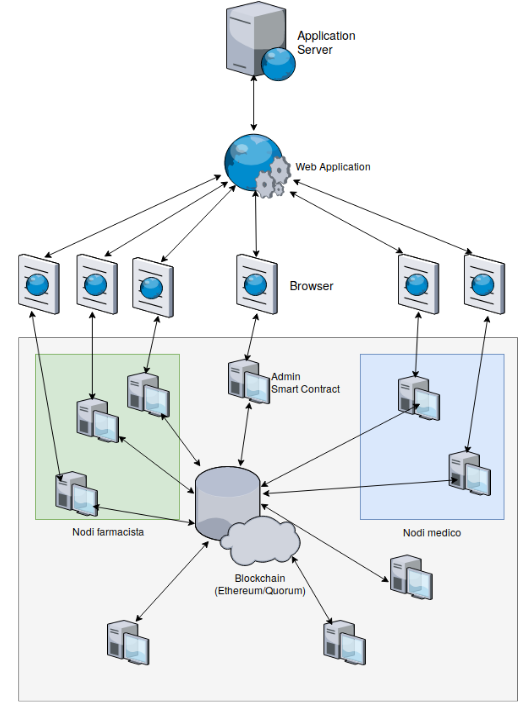
\includegraphics[width=.6\textwidth]{Implementazione/arch}
	%
	\caption{Diagramma del sistema}
	%
	\label{fig:diagramma del sistema}
	%
\end{figure}
%
Per gestire la prescrizione e l'erogazione delle ricette dematerializzate nonchè l'assegnazione dei ruoli all'interno della rete, la blockchain viene personalizzata mediante il deploy di uno specifico contratto di \textit{erogazione}, contenente la logica dell'applicazione. Gli utenti potranno interagire direttamente con la blockchain attraverso il proprio browser. L'applicazione decentralizzata è stata pensata come una \enquote*{single page application} con l'obiettivo di fornire una esperienza utente più fluida e simile alle applicazioni desktop dei sistemi operativi tradizionali. L'interfaccia è stata scritta utilizzando i linguaggi standard della programmazione web quali HTML5, CSS3 e JavaScript.
%
\section{Ricetta medica}
%
Il primo passo nell'implementazione dell'applicazione è stato quello di modellare l'oggetto "ricetta medica" secondo i requisiti enunciati. La ricetta medica dematerializzata si presenterà quindi in questo modo:
\begin{figure}[H]
	%
	\centering
	%
	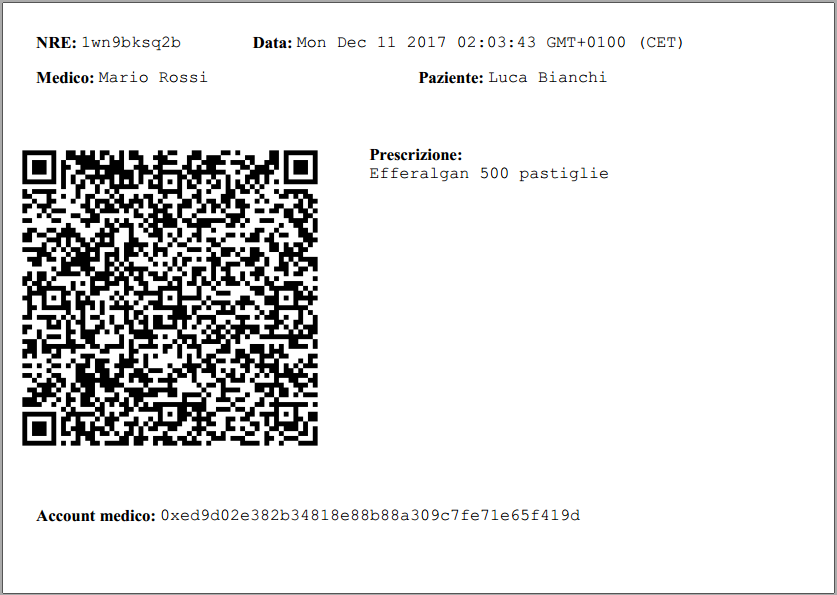
\includegraphics[width=.8\textwidth]{Implementazione/ricetta}
	%
	\caption{Struttura di una ricetta medica bianca dematerializzata}
	%
	\label{fig:struttura di una ricetta medica bianca dematerializzata}
	%
\end{figure}
ed è composta dai seguenti campi:
\begin{enumerate}
	\item \emph{NRE}. Codice univoco identificativo della ricetta dematerializzata. Viene utilizzato per ottimizzare la ricerca di una particolare ricetta all'interno della struttura dove vengono salvate.
	\item \emph{Timestamp}: rappresenta il timestamp preso all'atto della creazione della ricetta.
	\item \emph{Medico}: rappresenta il nome e il cognome del medico prescrittore.
	\item \emph{Paziente}: rappresenta il nome e il cognome del paziente.
	\item \emph{Prescrizione} rappresenta il contenuto della prescrizione.
	\item \emph{Qr-code}. Si è scelto di utilizzare il \gls{qrcode} come tecnologia per velocizzare l'erogazione della ricetta elettronica da parte dei farmacisti. Il farmacista andrà ad effettuare la scansione del qr-code per avviare il processo di erogazione della ricetta.
	\item \emph{Account Medico}: rappresenta l'indirizzo dell' account del medico prescrittore.
\end{enumerate}
Una volta ottenuta l'astrazione riguardante l'oggetto \enquote*{ricetta medica}, si è passati alla progettazione del contratto che regolasse la logica di funzionamento dell'applicazione sulla blockchain Quorum.
%
\section{Il contratto prescrizione}
%
La gestione della logica di funzionamento è stata realizzata mediante un contratto denominato \emph{Prescription.sol} caratterizzato dalle seguenti proprietà:
\begin{enumerate}
	\item una struttura per gestire i ruoli nel contratto (medico, farmacista e admin).
	\item una struttura per gestire le informazioni di un account. Nell'applicazione saranno composte per semplicità da nome, cognome e ruolo.
	\item una struttura per gestire le informazioni di una data ricetta. Nell'applicazione saranno composte da:
	      \begin{itemize}
	      	\item due variabili di tipo \emph{address}\footnote{Contiene un valore di 20 byte che corrisponde alla grandezza  indirizzo Ethereum} di cui una conterrà l'indirizzo sulla blockchain del medico prescrittore mentre l'altra onterrà l'indirizzo della farmacia che erogherà la farmacia. All'atto della creazione della ricetta questo dato particolare non è settato.
	      	\item una variabile di tipo \emph{bytes32} che conterrà il risultato dell'applicazione della primitiva crittografica \emph{Keccak-256 SHA3} sul contenuto della ricetta generata dal medico.
	      \end{itemize}
	\item per garantire invece che la modifica dello stato del contratto o l'invocazione delle funzioni del contratto vengano effettuate solo da determinati indirizzi, sono state inserite delle funzioni predefinite in Solidity denominate \emph{modifiers}. Ogni ruolo definito nel contratto ha la propria funzione modifiers associata in modo tale da poter garantire il corretto funzionamento del contratto. I modifiers vengono usate per modificare il corpo di una funzione e in particolare vengono preposti all'atto della chiamata della funzione per cui sono specificati. Il controllo ha successo solo se l'indirizzo che ha chiamato la funzione è del tipo giusto.
	\item il contratto infine contiene due strutture dati denominate \emph{mapping}. In Solidity un mapping  viene realizzato tramite la seguente sintassi $mapping (\textunderscore KeyType => \textunderscore ValueType) mapName$ dove \emph{\textunderscore KeyType} può essere la maggior parte dei tipo di dato\footnote{I tipi di dato non permessi come keyType sono mapping, array dinamici, struct ed enum} offerti in Solidity mentre \emph{\textunderscore ValueType} può essere qualsiasi tipo di dato. Questo tipo di dato può essere paragonato ad una tabella Hash. I due mapping sono stati definiti in accordo ai requisiti dell'applicazione in questo modo:
	      \begin{itemize}
	      	\item un mapping privato tra il codice univoco NRE e la struttura dati ricetta definita precedentemente. Questo mapping viene utilizzato per aumentare la velocità della ricerca della ricetta quando il farmacista procede ad effettuare il controllo su uno stato di una ricetta.
	      	\item un mapping privato tra l'indirizzo di un account sulla blockchain e la struttura contenente che gestisce le informazioni di un account.
	      \end{itemize}
	\item una serie di funzioni eseguibili che abilitano la logica del contratto. In particolare sono state implementate:
	      \begin{itemize}
	      	\item la funzione costruttrice del contratto che, all'atto del deploy sulla blockchain, setta l'account che effettua il deploy con il ruolo di amministratore. Si assume infatti che nella blockchain privata l'entità che procede al deploy del contratto sia l'entità di supervisione descritta nei capitoli precedenti.
	      	\item le funzioni per recuperare i dati anagrafici di un account.
	      	\item la funzione per recuperare il ruolo del mittente di una transazione.
	      	\item la funzione che permette di creare l'associazione tra nome, cognome, ruolo e indirizzo. A questa funzione viene associato il modifiers \emph{onlyAdmin}.
	      	\item la funzione per inserire una ricetta nella blockchain. Prende l'hash del contenuto della ricetta, l'nre associato e crea l'associazione con l'indirizzo che ha inviato la transazione che corrisponde al medico prescrittore. A questa funzione viene associato il modifiers \emph{onlyMedico}.
	      	\item la funzione che recupera una ricetta a partire dal NRE. Questa restituisce l'indirizzo del medico associato alla ricetta, il suo nre e l'hash. Nel caso in cui la ricetta non esiste nella blockchain verrà restituito il valore $0x0000000000000000000000000000000000000000$.
	      	\item la funzione che permette l'erogazione della ricetta da parte del farmacista. A partire dal NRE della ricetta va ad aggiornare il secondo campo address della ricetta inserendo l'indirizzo dell'account che l'ha appena erogata (quello della farmacia).
	      \end{itemize}
\end{enumerate}
%
\section{Creazione di una ricetta medica elettronica}
%
Abbiamo visto come, nella soluzione proposta, la ricetta dematerializzata viene concepita come un documento elettronico compilato dal medico prescrittore. Quest'ultimo infatti, tramite l'interfaccia specifica per il suo ruolo, andrà a riempire i campi della form corrispondenti alla ricetta elettronica. La pagina che viene presentata al medico è la seguente:
%
\begin{figure}[H]
	%
	\centering
	%
	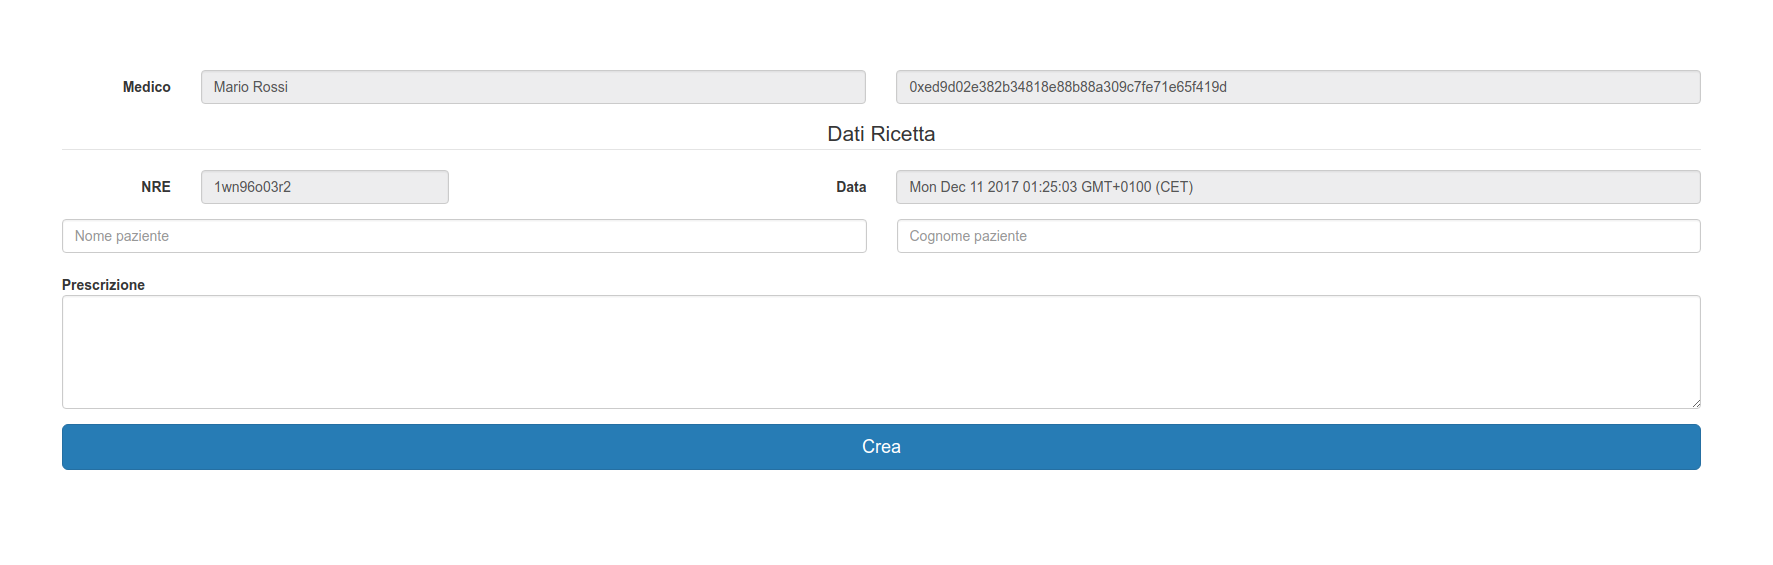
\includegraphics[width=1\textwidth]{Implementazione/prescrizione}
	%
	\caption{Schermata del medico prescrittore}
	%
	\label{fig:schermata del medico prescrittore}
	%
\end{figure}
%
Alcuni campi della form sono riempiti automaticamente e non possono essere modificati dal medico. In particolare le informazioni relative al nome e cognome del medico sono recuperate a partire dalla sessione di Web3.js attiva all'interno del browser (permette al browser di interagire direttamente con il contratto e la blockchain) mentre il timestamp viene generato lato client e il codice univoco NRE viene ricevuto dall'application server (tramite Express). La creazione di una ricetta elettronica da parte di un medico avviene nel modo seguente:
\begin{enumerate}
	\item All'atto del caricamento della pagina del medico, l'application server provvede a generare ed inviare un nuovo NRE al client.
	\item Il medico provvede a riempire i campi della form della ricetta elettronica.
	\item Una volta riempiti tutti i campi il medico provvede a creare la ricetta cliccando sul bottone \enquote*{crea}. Il submit della form avvierà la seguente sottoprocedura (il dialogo con la blockchain è asincrono):
	      \begin{enumerate}
	      	\item viene parsato il campo data al fine di renderlo adatto alla trasmissione.
	      	\item tutti i campi della ricetta vengono serializzati in un oggetto json. 
	      	\item l'oggetto json viene convertito in stringa per potervi applicare la primitiva crittografica sha3\footnote{Ethereum vuole una stringa come argomento da passare a questa api} messa a disposizione da Ethereum tramite le sue api. 
	      	\item a questo punto viene effettuata una transazione in quanto si va a chiamare la funzione del contratto che si occupa dell'inserimento di una ricetta sulla blockchain.
	      	\item una volta ottenuto il riscontro effettivo dell'avvenuto inserimento della ricetta sulla blockchain viene effettuata una chiamata post verso l'application server al quale viene passato lo stesso oggetto serializzato inviato sulla blockchain. 
	      	\item il server andrà prima a creare la struttura della ricetta elettronica (un documento in formato B6 landscape) inserendo tutti i campi come abbiamo visto nei paragrafi precedenti e, successivamente, andrà a creare il qr-code\footnote{Per la generazione del qr-code si è scelta una tra le tante librerire disponibili per Node. In questo caso \emph{qr-image}ancona17} contenente la stringa generata a partire dal json serializzato (così come è avvenuto nello step precedente) e lo inserirà all'interno della ricetta elettronica. Una volta generata la ricetta elettronica il server invierà il risultato al client permettendo al medico di salvare la ricetta elettronica oppure di creare una nuova ricetta. Si è scelto di dare la possibilità di stampa della ricetta dematerializzata (ripristinando così il promemoria essitente) per similitudine rispetto al sistema attuale tuttavia la scansione del qr-code può anche essere fatta tramite ricetta elettronica su smartphone permettendo così l'abbandono completo della carta nel processo di prescrizione delle ricette mediche.
	      \end{enumerate}
\end{enumerate}
Il procedimento appena descritto viene inoltre mostrato nel seguente diagramma delle sequenze:
%
\begin{figure}[H]
	%
	\centering
	%
	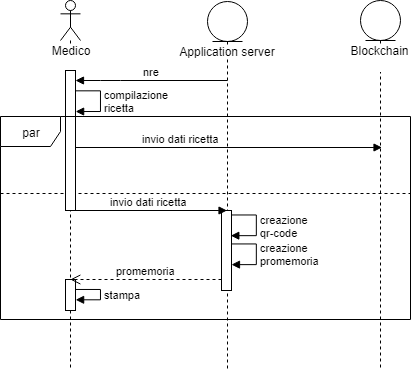
\includegraphics[width=.9\textwidth]{Implementazione/prescrizioneSeq}
	%
	\caption{Creazione di una ricetta dematerializzata}
	%
	\label{fig:creazione di una ricetta dematerializzata}
	%
\end{figure}
%
\section{Erogazione di una ricetta elettronica}
%
Una volta che la ricetta viene correttamente salvata sulla blockchain e viene generato il corretto promemoria elettronico (ed eventualmente stampato) per il paziente, quest'ultimo può recarsi in una farmacia per richiedere l'erogazione della prescrizione che ha appena ricevuto. Come avviene per il medico prescrittore anche per il farmacista è stata un'interfaccia esclusiva per il suo ruolo così fatta:
%
\begin{figure}[H]
	%
	\centering
	%
	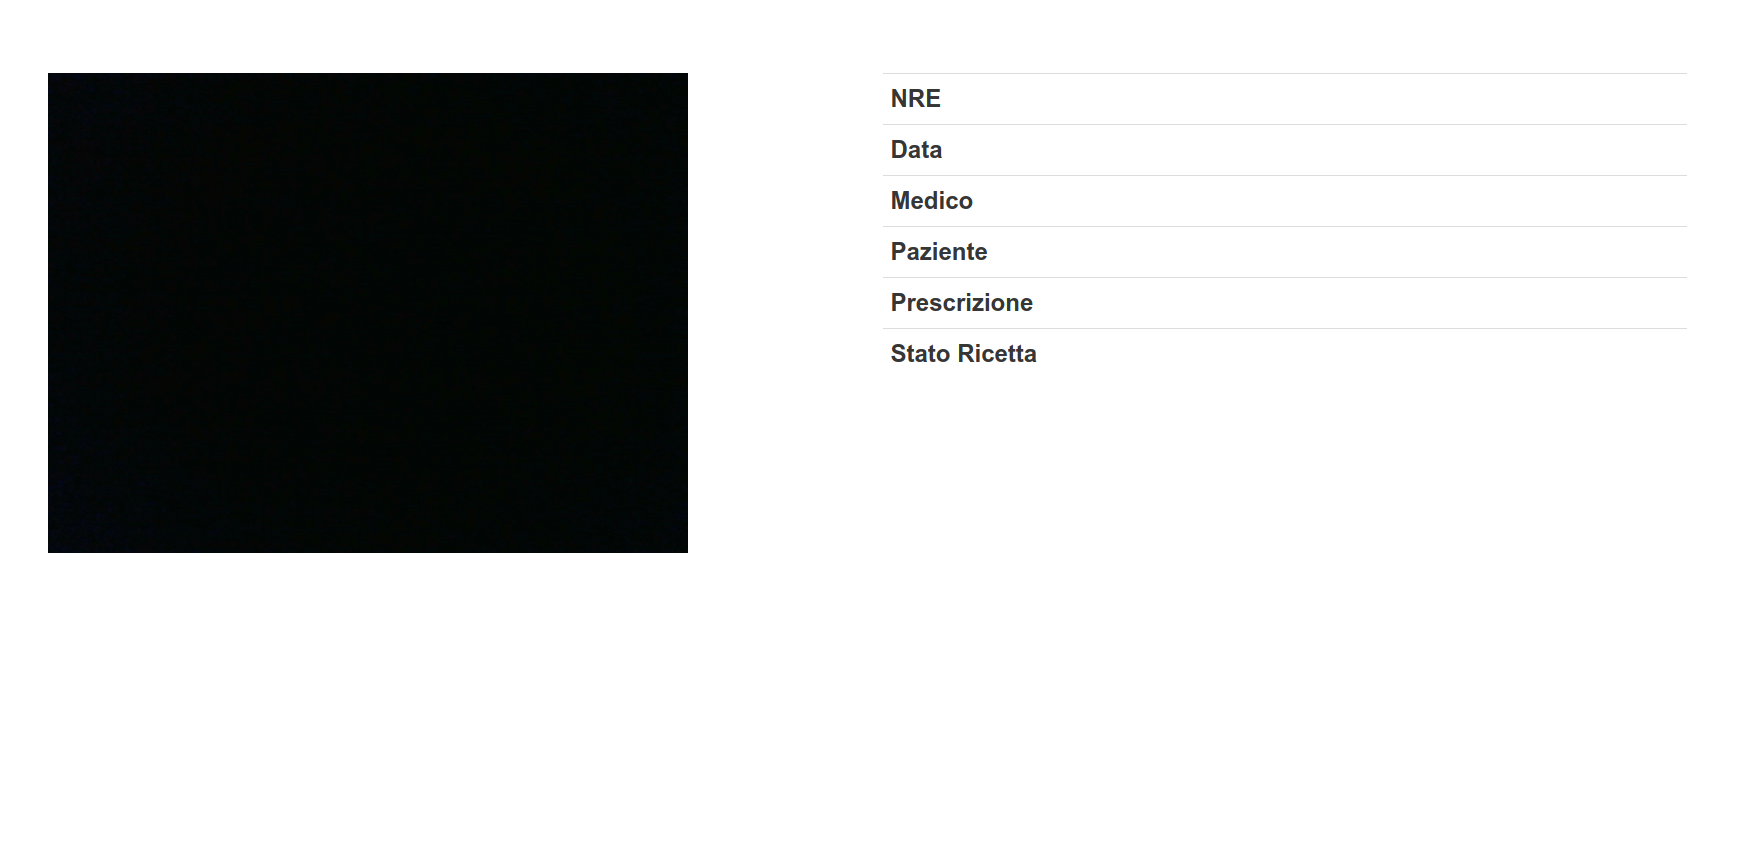
\includegraphics[width=1\textwidth]{Implementazione/farmacia}
	%
	\caption{Schermata del farmacista}
	%
	\label{fig:schermata del farmacista}
	%
\end{figure}
L'interfaccia è stata divisa in due zone:
\begin{itemize}
	\item Il box di sinistra andrà a contenere il feed della webcam. Sia per velocizzare la procedura di erogazione che per minimizzare l'errore dell'operatore (non è più necessario inserire i campi della ricetta manualmente per cercarla ed erogarla) è stato implementato uno scanner di codici qr-code che interagisce direttamente con la webcam del terminale dell'operatore. \\
	      Lo scanner di qr-code è stato implementato completamente mediante HTML5 (HTML5 compliant) per renderlo il più possibile compatibile con i browser attuali senza il bisogno di installare tecnologie abilitanti di terze parti (e.g. Flash player di Adobe).
	\item la griglia di destra invece viene automaticamente popolata all'atto della scansione del qr-code andando quindi a contenere il riassunto, mostrato a schermo, del contenuto della ricetta estratto dal codice appena scansionato.
\end{itemize}
L'erogazione di una ricetta da parte del farmacista avviene nel seguente modo:
\begin{enumerate}
	\item All'atto del caricamento della pagina del farmacista viene avviato lo scanner del qr-code e il suo feed sarà mostrato sull'interfaccia.
	\item Nel momento in cui si va a scansionare un codice qr-code contenuto sulla ricetta elettronica il client provvederà a parsare il contenuto del qrcode per popolare la griglia e preparare i dati per la ricerca della ricetta sulla blockchain.
	\item Una volta ottenuti tutti i campi della ricetta, il client ricrea la stringa che il client del medico prescrittore ha generato all'atto della creazione. Questo viene fatto perchè l'hash creato dal farmacista tramite i campi appena scansionati sarà confrontato con l'hash salvato dalla blockchain dal medico. Per far questo il client chiamerà la funzione del contratto addetta alla ricerca di una determinata ricetta medica passandogli il codice univoco NRE. La ricerca può avere due esiti diversi:
	      \begin{itemize}
	      	\item La ricetta non viene trovata. La funzione di ricerca restituisce valore $0x0000000000000000000000000000000000000000$ e il client notifica al farmacista che la ricetta che sta valutando non è valida in quanto non presente nella blockchain. Questo esito viene mostrato nella seguente figura:
	      	      %
	      	      \begin{figure}[H]
	      	      	%
	      	      	\centering
	      	      	%
	      	      	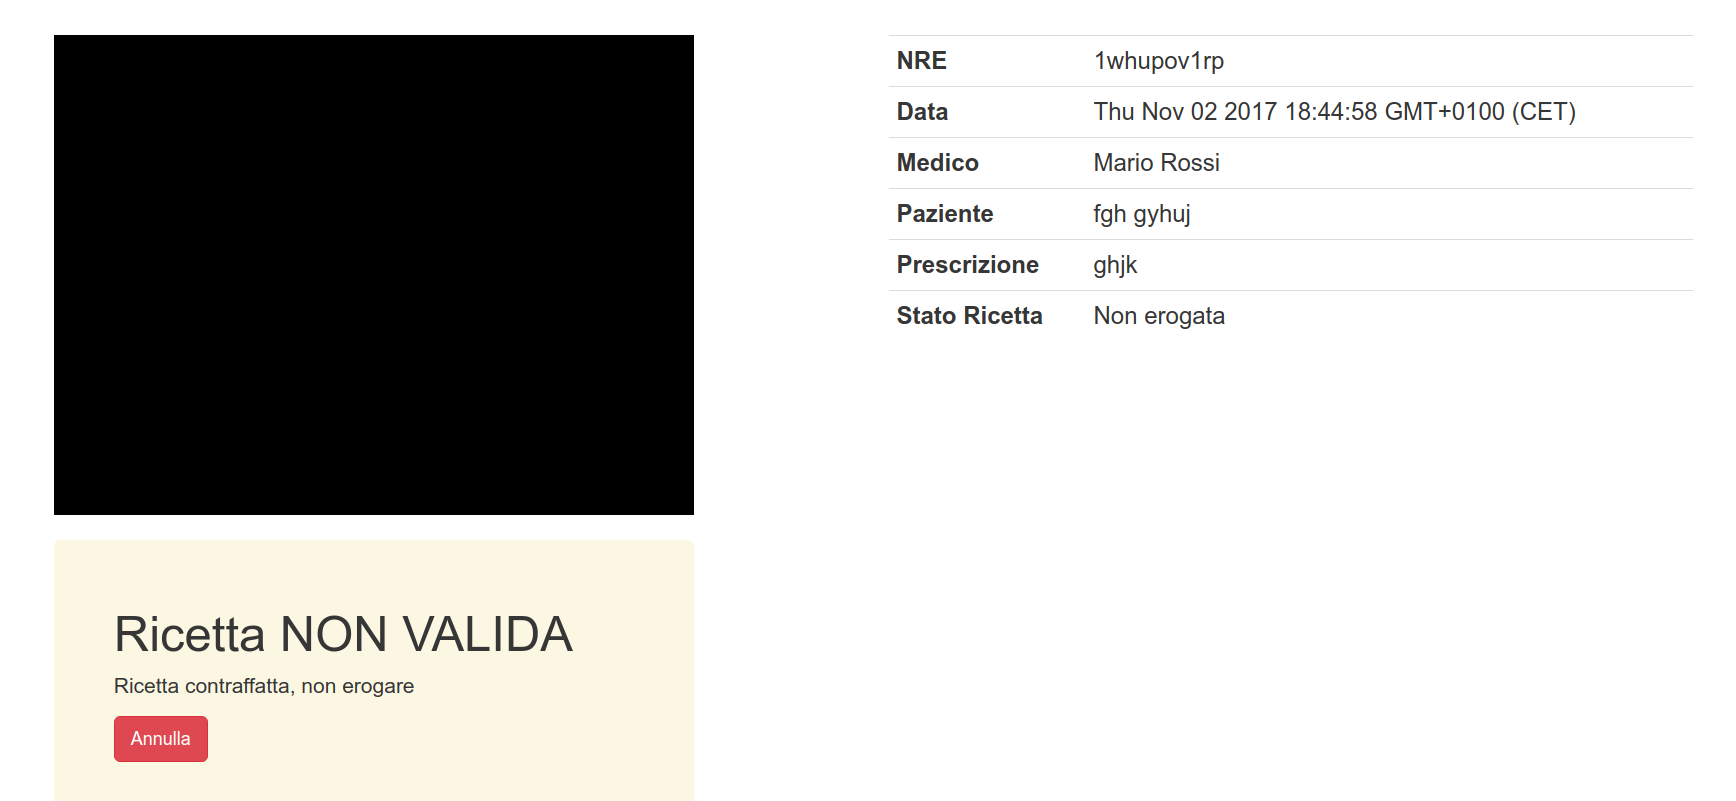
\includegraphics[width=.7\textwidth]{Implementazione/ricettaNO}
	      	      	%
	      	      	\caption{Ricetta medica non valida}
	      	      	%
	      	      	\label{fig:ricetta medica non valida}
	      	      	%
	      	      \end{figure}
	      	      %
	      	\item la ricetta viene trovata all'interno della blockchain e il risultato della transazione è un oggetto che contiene l'account del medico prescrittore, l'hash della ricetta e il suo stato(se è stata o meno già erogata). 	      
	      \end{itemize}
	\item L'hash della ricetta creato dal farmacista sarà ora confrontato con l'hash della ricetta ricevuto dalla blockchain come prova di integrità e non manomissione del contenuto della ricetta. I possibili risultati di questo confronto sono:
	      \begin{itemize}
	      	\item Ricetta valida. Il contenuto della ricetta corrisponde a quello salvato nella blockchain e non è già stata erogata. Il farmacista può procedere all'erogazione andando ad aggiornare lo stato della ricetta salvato sulla blockchain. Questa situazione viene mostrata nella seguente figura: 
	      	      %
	      	      \begin{figure}[H]
	      	      	%
	      	      	\centering
	      	      	%
	      	      	\includegraphics[width=.7\textwidth]{Implementazione/farmaciaOk}
	      	      	%
	      	      	\caption{Ricetta medica valida}
	      	      	%
	      	      	\label{fig:ricetta medica valida}
	      	      	%
	      	      \end{figure}
	      	      %
	      	\item La ricetta è valida ma è già stata erogata. Non è concessa la possibilità di erogare una seconda volta la ricetta elettronica. Questa situazione viene mostrata nella seguente figura: 
	      	      %
	      	      \begin{figure}[H]
	      	      	%
	      	      	\centering
	      	      	%
	      	      	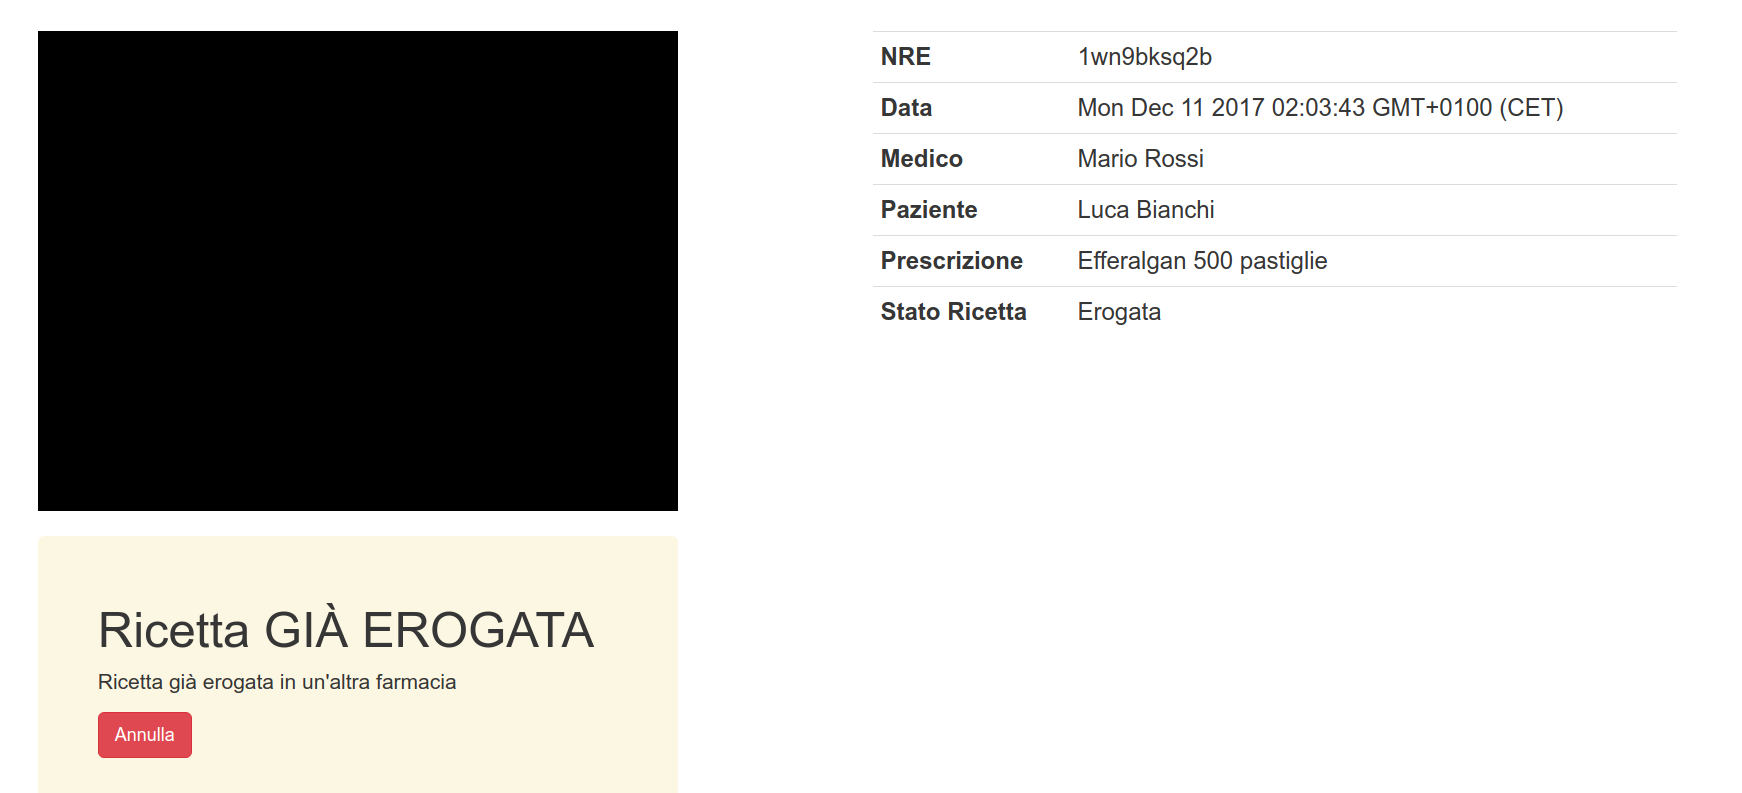
\includegraphics[width=.7\textwidth]{Implementazione/ricettaUSATA}
	      	      	%
	      	      	\caption{Ricetta medica già erogata}
	      	      	%
	      	      	\label{fig:ricetta medica già erogata}
	      	      	%
	      	      \end{figure}
	      	      %
	      	\item Ricetta medica non valida. Il contenuto della ricetta è stato alterato in qualche modo. L'erogazione viene rifiutata e la ricetta viene considerata non valida. Viene mostrata la stessa schermata di errore vista nel caso in cui la ricetta non viene trovata, ma con un codice di errore diverso.
	      \end{itemize}
\end{enumerate}
Il procedimento appena descritto viene inoltre mostrato nel seguente diagramma delle sequenze:
%
\begin{figure}[H]
	%
	\centering
	%
	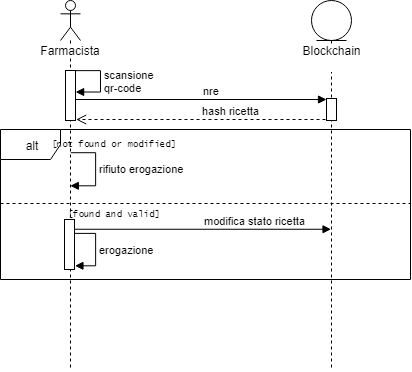
\includegraphics[width=.9\textwidth]{Implementazione/erogazioneSeq}
	%
	\caption{Creazione di una ricetta dematerializzata}
	%
	\label{fig:creazione di una ricetta dematerializzata}
	%
\end{figure}
%  	 
\section{Registrazione di nuovi account}
%
L'ammministratore presente all'interno della blockchain ha l'unico compito di gestire le associazioni tra gli indirizzi degli account presenti sulla catena e il ruolo che essi andranno a ricoprire nell'applicazione. La sua figura è stata inserita per avere una gestione più rapida del mapping account-ruolo, considerando anche il fatto che una figura di supervisione, seppur senza possibilità di fare altre azioni, sia necessaria in quanto stiamo parlando di un ambito sanitario nazionale La sua schermata è la seguente:
%
\begin{figure}[H]
	%
	\centering
	%
	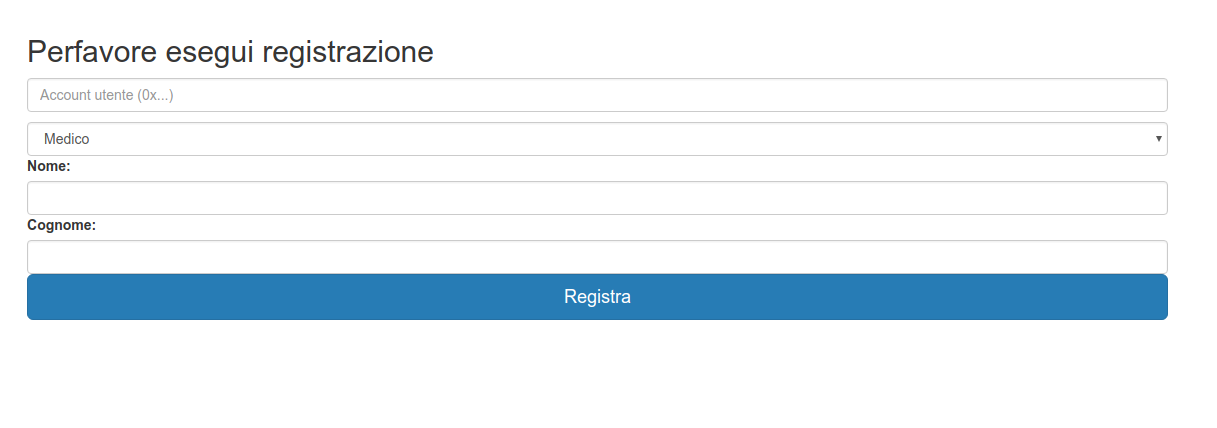
\includegraphics[width=.9\textwidth]{Implementazione/admin}
	%
	\caption{Assegnazione del ruolo da parte dell'amministratore}
	%
	\label{fig:assegnazione del ruolo da parte dell'amministratore}
	%
\end{figure}
% 
 
%
% ------------------------------------------------------------------------ %
% !TEX encoding = UTF-8 Unicode
% !TEX TS-program = pdflatex
% !TEX root = ../Tesi.tex
% !TEX spellcheck = it-IT
% ------------------------------------------------------------------------ %
%
% ------------------------------------------------------------------------ %
% 	NOME CAPITOLO
% ------------------------------------------------------------------------ %
%
\chapter{Considerazioni sulla sicurezza \& conclusioni}
%
\label{cap:conclusioni}
%
\section{Sicurezza}
%
Quello realizzato nel corso dell'attività di tesi è un prototipo di un'applicazione per ricette mediche bianche dematerializzate che risponde ai \emph{Requisiti centrati sulle informazioni}\footnote{Modello CIA}ovvero quei requisiti informali che esprimono come dovrebbero essere gestite le informazioni all'interno di un sistema informatico. Questi requisiti sono:
\begin{enumerate}
	\item \emph{confidenzialità}: le informazioni devono essere accessibili solo a coloro che sono autorizzati. Questo è stato realizzato mediante l'utilizzo di una blockchain permissione privata che supporta sia transazioni pubbliche e private e non è interrogabile dall'esternon se non previa autorizzazione dell'autorità di supervisione. Inoltre il dato sensibile corrispondente al contenuto della ricetta elettronica non viaggia mai in chiaro sulla blockchain, ma quello che vedrebbe un eventuale utente malevolo sarebbe l'hash della ricetta.
	\item \emph{integrità}: le informazioni possono essere modificate solo da coloro che sono autorizzati. Questo requisito viene gestito a livello di logica di contratto tramite i modifier di accesso che vengono preposti alle transazioni quando si va ad interagire con l'inserimento della ricetta nella blockchain. L'applicazione supporta una divisione di ruoli che può essere eventualmente estesa per adattarsi alle nuove esigenze applicative.
	\item \emph{disponibilità}: le informazioni devono essere sempre accessibili in qualsiasi momento a coloro che ne hanno l'autorità o il permesso. Questa è una proprietà intrinseca della blockchain, data la sua natura decentralizzata.
\end{enumerate}
Inoltre l'applicazione risponde ai \emph{requisiti centrati sulle persone}\footnote{Modello AAA} ovvero quei requisiti informali che esprimono i vincoli a cui dovrebbero essere soggetti gli individui che interagiscono con i sistemi informatici. Questi requisiti sono:
\begin{enumerate}
	\item \emph{autenticazione}: le persone devono provare la loro identità. Questo requisito viene supportato dalla tipica gestione degli account nella blockchain che sono identificati ed agiscono mediante la loro coppia di chiave pubblica-chiave privata. Ogni browser verrà configurato per utilizzare un solo account precedentemente autorizzato e le chiavi saranno conservate in modo sicuro. Al momento della scrittura del lavoro di tesi i modi possibili per raggiungere questo scopo sono:
	      \begin{itemize}
	      	\item  l'utilizzo di un programma denominato "Metamask" compatibile con i maggiori browser in commercio, che permette di interagire con la blockchain dopo aver correttamente importato l'account mediante la chiave privata corrispondente (questo è possibile perchè in Metamask è capace di iniettare la sessione di web3.js all'interno del browser, permettendo così di effettuare transazioni da e verso la blockchain tramite l'account configurato in esso). Metamask è un programma di tipo "sandbox" ovvero una volta che è stata importata la chiave privata, se questa viene perduta risulta impossibile recuperarla tramite questo programma. 
	      	\item l'utilizzo di un browser modificato denominato "Mist". Attualmente si presenta come la principale alternativa ai browser in commercio. Mist ha già integrate tutte le librerie necessare per dialogare ed interagire con le blockchain e le applicazioni decentralizzate su di essa senza l'aggiunta di ulteriori programmi. A suo svantaggio va il fatto che deve essere configurato per interagire con le blockchain private (può risultare problematico) e rimane un programma con cui l'utente non ha familiarità.
	      \end{itemize}
	\item \emph{autorizzazione}. Le persone devono poter accedere ad una risorsa solo se autorizzate. Questo viene gestito ed implementato nella logica di contratto a livello di ruolo del singolo account.
	\item \emph{non ripudio}. Le persone devono essere responsabili delle proprie azioni e, in particolare, non possono negare quanto affermato precedentemente. Questo viene intrinsecamente supportato dalla blockchain in quanto ogni transazione viene firmata dal mittente (che sia essa pubblica o privata). Inoltre nel contratto sono state inseriti delle strutture dati come ulteriore traccia delle associazioni tra ruolo-account e account-ricetta.
\end{enumerate}
%
\subsection{Application server}
All'interno dell'architettura decentralizzata è stata valutato ed implementato un elemento application server, un elemento tipico delle architetture client-server. Questa scelta che in prima istanza sembra vada ad inficiare l'implementazione decentralizzata è risultato necessario per questioni di sicurezza. Infatti il codice lato client, nonostante tutte le tecniche per pervenire XSS\footnote{Cross-Site-Scripting} e di offuscamento del codice, risulta sempre vulnerabile all'injection tramite la console del browser. Allora la logica di generazione della ricetta elettronica è stata spostata server-side (Express) al fine di evitare la modifica della logica di generazione di ricetta dematerializzata da parte di un utente malevolo e preservare così l'integrità dei file generati dal medico. Lo svantaggio di questa entità è che si comporta a tutti gli effetti come un \emph{Single point of failure} ed è necessario prendere provvedimenti al livello di:
\begin{itemize}
	\item gestione del carico del server tramite l'inserimento di load balancer (evitare i colli di bottiglia).
	\item gestione della disponibilità del server in caso di \gls{dos}\footnote{Denial of service} tramite l'applicazione di tecniche di tolleranza ai guasti (tecniche di replicazione e duplicazione).
\end{itemize}
%
\section{Conclusioni}
%
La scelta di una blockchain privata come Quorum, anche se complessa dal punto di vista della configurazione, risulta estremamente versatile nella gestione di sistemi complessi decentralizzati in cui sono necessarie determinati livelli di sicurezza. Inoltre si presenta anche come una valida soluzione per sviluppare software blockchain-based la cui logica risieda all'interno di contratti che vengono eseguiti sulla stessa blockchain dato che contiene dentro di se tutte le feature di Ethereum. \\
Inoltre l'utilizzo della tecnologia della blockchain si presenta come una valida alternativa all'utilizzo dei database tradizionali perchè sotto determinati requisiti riesce ad offrire maggiori garanzie rispetto ad essi. Infatti, anche se presente un'entità supervisionante, non sono presenti intermediari durante l'interazione tra gli attori principali del sistema (medici e farmacisti) e chiunque possiede l'autorizzazione (sia di ruolo che di peer) può interagire con le informazioni sulla blockchain mentre questo non è possibile nei database tradizionali dove solo l'autorità centrale può accedere ai nostri dati. \\
Inoltre, mentre nei database tradizioni risulta necessario applicare attivamente tecniche di replicazione e di tolleranza ai guasti, nella blockchain questo è intrinseco nell'architettura stessa. Perciò la scelta riguardante quale tecnologia da utilizzare deve essere presa in relazione agli obiettivi che si vogliono raggiungere.
\subsection{Soluzione offerta}
Nel merito dell'applicazione implementata per la gestione di ricette elettroniche dematerializzate sono stati raggiunti i seguenti obiettivi principali:
\begin{itemize}
	\item \textit{\textbf{performance}}: rispetto alla controparte pubblica una blockchan privata offre performance maggiori in quanto utilizza meccanismi di consenso più adatti ad un ambiente permissioned e meno pesanti computazionalmente come la POW.
	\item \textit{\textbf{disponibilità}}: essendo una struttura di tipo peer-to-peer che cresce con l'aumentare degli utenti che partecipano all'attività al suo interno la possibilità di avere informazioni sempre disponibili aumenta.
	\item \textit{\textbf{aggiornamento}}: la blockchain risulta sempre aggiornata perchè le transazioni vengono sempre propagate attraverso i nodi, siano esse pubbliche o private.
	\item \textit{\textbf{affidabilità}}: il corretto funzionamento delle attività di mining viene supervisionato da un entità garante soprattutto nel caso di informazioni sensibili come i dati medico-sanitari.
	\item \textit{\textbf{resilienza ai guasti}}: la blockchain è intrinsecamente resiliente ai guasti.
\end{itemize} 
%
\appendix
%
% ------------------------------------------------------------------------ %
% !TEX encoding = UTF-8 Unicode
% !TEX TS-program = pdflatex
% !TEX root = ../Tesi.tex
% !TEX spellcheck = it-IT
% ------------------------------------------------------------------------ %
%
% ------------------------------------------------------------------------ %
% 	NOME APPENDICE 1
% ------------------------------------------------------------------------ %
%
\chapter{Block Header Ethereum}
%
\label{cap:blockheader}
%
\begin{figure}[H]
	%
	\centering
	%
	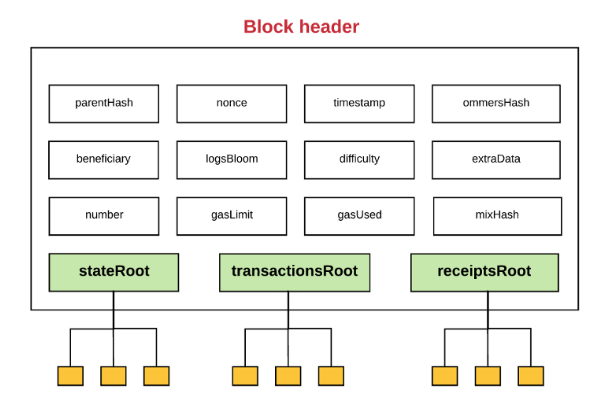
\includegraphics[width=.8\textwidth]{Ethereum/blockHeader}
	%
	\caption{Schema Blocco in Ethereum}
	%
	\label{fig:schema blocco in Ethereum}
	%
\end{figure}
In ethereum un blocco è composto da:
\begin{itemize}
	\item il block header;
	\item le informazioni che riguardano l'insieme delle transazioni incluse nel blocco;
	\item un insieme di altri block header per l'attuale block ommers. Con \enquote*{ommer} o \enquote*{uncle block} si intende un figlio di un antenato che non è un antenato. Se A è uncle di B, B è nipote di A. Questi sono necessari per aiutare a ricompensare i miners quando sono trovate soluzioni duplicate di blocchi a causa dei tempi di blocco più corti di Ethereum (rispetto a Bitcoin ad esempio). Un uncle è una ricompensa più piccola rispetto ad un full block (se sono inviati oltre il blocco successivo, la ricompensa decresce rapidamente fino a zero dopo sette blocchi).
\end{itemize}%
La parte che contiene la maggior parte delle informazioni per il corretto funzionamento della blockchain è il block header. Esso è composto da:
\begin{enumerate}
	\item parentHash: l'\gls{hash} del block header genitore (questo è quello che rende l'insieme di blocchi una catena);
	\item ommersHash: l'hash della corrente lista di block ommers;
	\item beneficiary: l'indirizzo dell'account che riceve la ricompensa per minare il blocco;
	\item stateRoot: struttura dati di tipo Tree. Contiene l'hash del root node dello state tree (così è facile per i light client verificare gli stati);
	\item transactionsRoot: struttura dati di tipo Tree. Contiene l'hash del root node del tree che contiene tutte le transazioni listate nel blocco;
	\item receiptsRoot: struttura dati di tipo Tree. Contiene l'hash del root node del tree che contiene le ricevute di tutte le transazioni listate nel blocco;
	\item logsBloom: una struttura dati che contiene informazioni di log;
	\item difficulty: indica il livello di difficoltà del blocco;
	\item number: il numero del blocco corrente (il genesis block ha numero di blocco 0);
	\item gasLimit: l'attuale gasLimit per blocco;
	\item gasUsed: la somma del gas totale usato dalle transazioni in questo blocco;
	\item timestamp: iltimestamp unix dell'inception di questo blocco;
	\item extraData: dati extra relativi a questo blocco;
	\item mixHash: un hash che, quando combinato con il nonce, dimostra che questo blocco ha portato avanti sufficiente computazione;
	\item nonce: un hash che, quando combinato con il mixHash, dimostra che questo blocco ha portato avanti sufficiente computazione.
\end{enumerate}%

%
% ------------------------------------------------------------------------ %
% !TEX encoding = UTF-8 Unicode
% !TEX TS-program = pdflatex
% !TEX root = ../Tesi.tex
% !TEX spellcheck = it-IT
% ------------------------------------------------------------------------ %
%
% ------------------------------------------------------------------------ %
% 	NOME APPENDICE 2
% ------------------------------------------------------------------------ %
%
\chapter{Schema transazioni Quorum}
%
\label{cap:transaction}
%
La figura mostra come viene processata una transazione privata in Quorum:
%
\begin{figure}[H]
	%
	\centering
	%
	\includegraphics[width=.9\textwidth]{Quorum/transaction}
	%
	\caption{Schema di una transazione privata Quorum}
	%
	\label{fig:schema di una transazione privata quorum}
	%
\end{figure}
%
\begin{enumerate}
	\item il party A invia una transazione al proprio nodo Quorum, specificando il payload della transazione e settando il \enquote*{privateFor} con la chiave pubblica per i gruppi A e B.
	\item il nodo Quorum del party A passa la transazione al relativo gestore delle transazioni, richiedendogli di memorizzare il payload.
	\item il transaction manager del party A chiama il proprio Enclave associato per validare il mittente e crittare il payload.
	\item l'Enclave del party A controlla la chiave privata\footnote{\gls{asimmetrica}} del party A e, una volta validata, effettua la conversione della transazione. Questo comporta: 
	      \begin{enumerate}
	      	\item generazione di chiave simmetrica e random nonce.
	      	\item crittografia del payload della transazione e del nonce con la chiave simmetrica dello step precedente.
	      	\item calcolo SHA3-512 del payload del passo precedente.
	      	\item iterazione attraverso la lista dei destinatari della transazione, in questo caso i party A e B, crittando la chiave simmetrica dello step precedente con la chiave pubblica del destinatario (PGP). 
	      	\item viene ritornato il payload crittografato allo step 4.2, l'hash dello step 4.3 e la chiave crittografata (per ogni destinatario) dello step precedente al transaction manager.
	      \end{enumerate}
	\item il transaction manager del party A immagazzina il payload (criptato con la chiave simmetrica) e la chiave simmetrica criptata utilizzando l'hash come indice e poi trasferendo in modo sicuro: hash, payload criptato e la chiave simmetrica criptata con la chiave pubblica del party B al transaction manager del party B. Quest'ultimo risponderà con una risposta di tipo ack/nack. Se il party A non riceve risposta o riceve nack dal party B allora la transazione non sarà propagata nella rete.
	\item una volta che la trasmissione dei dati al transaction manager del party B ha avuto successo il transaction manager del party A ritorna l'hash al nodo Quorum, il quale hash va a rimpiazzare il payload originale della transazione e cambia il valore \emph{V} della transazione in 37 o 38. Questo valore indicherà agli altri nodi che questo hash rappresenta una transazione privata con un payload associato criptato.
	\item a questo punto la transazione è propagata al resto della rete utilizzando il protocollo P2P standard di Ethereum.
	\item un blocco contenente la transazione AB è creato e distribuito ad ogni party sulla rete.
	\item Elaborando il blocco tutti i party proveranno a processare la transazione. Ogni nodo Quorum riconoscerà un valore \emph{V} di 37 o 38, identificandola quindi come transazione il cui payload deve essere decrittato, ed effettuerà una chiamata al proprio transaction manager per determinare se possiedono la transazione (utilizzando l'hash come indice per cercare).
	\item dato che il party C non possiede la transazione riceverà un messaggio \enquote*{NotRecipient} e salterà la transazione non aggiornando il suo stateDb privato. Invece la ricerca da parte dei party A e B avrà esito positivo identificando quindi il fatto che posseggono la transazione e procederanno a chiamare il proprio Enclave passando il payload criptato, la chiave simmetrica criptata e la firma.
	\item Enclave valida la firma e poi decritta la chiave simmetrica utilizzando la chiave privata del party (posseduta da Enclave) , decritta il payload della transazione utilizzando la chiave simmetrica appena ottenuta e ritorna il payload decrittato al transaction manager.
	\item il transaction manager dei party A e B allora invia il payload decrittato all'EVM per l'esecuzione del codice del contratto. Questa esecuzione aggiornerà solo il private stateDB del nodo Quorum. Una volta che il codice è stato eseguito, viene eliminato per far sì che non sia disponibile a meno di rieseguire il processo di decrittazione
\end{enumerate} 
%
% ------------------------------------------------------------------------ %
% !TEX encoding = UTF-8 Unicode
% !TEX TS-program = pdflatex
% !TEX root = ../Tesi.tex
% !TEX spellcheck = it-IT
% ------------------------------------------------------------------------ %
%
% ------------------------------------------------------------------------ %
% 	NOME APPENDICE 3
% ------------------------------------------------------------------------ %
%
\chapter{Conseus Process Flow}
%
\label{cap:conseus}
%
%
\begin{figure}[H]
	%
	\centering
	%
	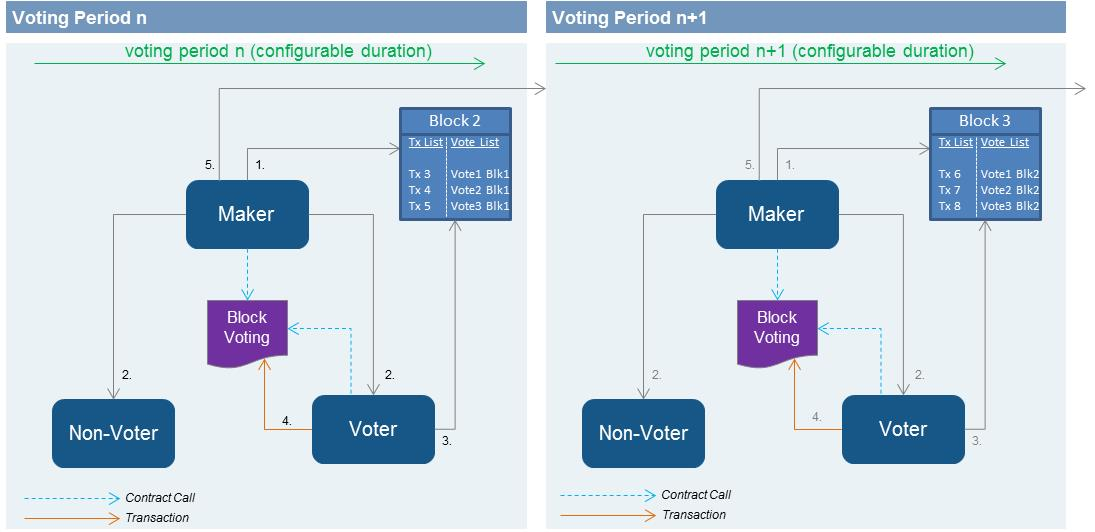
\includegraphics[width=.9\textwidth]{Quorum/conseus}
	%
	\caption{Flusso del consenso in Quorum}
	%
	\label{fig:flusso del consenso di quorum}
	%
\end{figure}
%
All'interno di un periodo:
\begin{enumerate}
	\item Il maker node che raggiunge il timeout per primo crea il blocco e lo firma. Il blocco include i voti per il blocco genitore che sono stati trasmessi nel precedente periodo.
	\item Il blocco viene pubblicato sulla rete utilzizando lo standard P2P Ethereum Protocol. Tutti i nodi ricevono il blocco, a prescindere dal loro ruolo.
	\item I Voters validano il blocco. Questo include:
	      \begin{enumerate}
	      	\item Chiamata al contratto BlockVoting per controllare se il maker può effettivamente creare il blocchi (i.e. ha il ruolo maker).
	      	\item Chiamata al contratto BlockVoting per controllare se il blocco genitore del blocco in valutazione ha ricevuto abbastanza voti.
	      	\item Vengono eseguite tutte le transazioni processabili nel blocco ovvero le transazioni pubbliche e quelle private del insieme di partecipanti di cui fa parte il nodo (questo dopo aver recuperato il payload transaciont dal Transaction Manager).
	      	\item Viene validato lo stato pubblico comparando il \emph{Public state root hash} con lo \emph{State root} all'interno del blocco.
	      	\item Viene effettuato l'hash di tutte le transazioni del blocco (sia pubbliche che private) e viene quindi confrontato con il \emph{transaction hash} del blocco. Questo viene realizzato per assicurarsi che tutti i Voters concordino sulla lista delle transazioni nel blocco.
	      \end{enumerate}
	\item Una volta validato con successo, i nodi Voters inviano il proprio voto al contratto BlockVoting usando una transazione Ethereum standard che viene distribuita su tutti i nodi. Dato che i voti per un dato blocco sono trasmessi tramite transazioni standard, possono essere processati solo quando il blocco successivo è stato creato.
	\item I maker node raggiungono il proprio timeout, determinano se il numero minimo di voti è stato raggiungo per il blocco precedente e poi la procedura di creazione del blocco$->$validazione$->$votazione viene ripetuta.
\end{enumerate}%
Mentre il consenso sullo stato privato è implicito e viene ottenuto attraverso una combinazione sincronizzata di input di contratti (\emph{Global Transaction Hash Validation Check}), un EVM deterministico (\emph{Public State Validation Check}), sincronizzazione della catena (nuovi blocchi aggiunti solo alla catena canonica) è possibile validare ulteriormente il consenso sullo stato privato tramite il comdanto Quorum \emph{eth\_StorageRoot}. Questo comando infatti restituisce il \emph{Private State Root Hash} di un account contratto ad un dato numero di blocco che può quindi essere validato rispetto al risultato dello storageRoot di una controparte fuori dalla catena o a livello di applicazione. Questa risulta un'ulteriore forma di sicurezza sulle transazioni private implementata dagli sviluppatori di Quorum. %
 
%
% ------------------------------------------------------------------------ %
% !TEX encoding = UTF-8 Unicode
% !TEX TS-program = pdflatex
% !TEX root = ../Tesi.tex
% !TEX spellcheck = it-IT
% ------------------------------------------------------------------------ %
%
% ------------------------------------------------------------------------ %
%   NOME APPENDICE 4
% ------------------------------------------------------------------------ %
%
\chapter{Script di configurazione}
%
\label{cap:codici}
%
Questo capitolo conterrà tutti gli script di configurazione, utilizzati nell'ambito dell'implementazione dell'applicazione e citati nel capitolo \autoref{cap:implementazione}.
%
\section{Vagrant}
%
\label{cap:vagrantConfig}
%
Il VagrantFile utilizzato nello sviluppo:\newline
\begin{center}
	\begin{lstlisting}[language=ruby,caption={VagrantFile del progetto},captionpos=b,frame=lines,basicstyle=\linespread{0.9}\small]
Vagrant.configure(2) do |config|
  config.vm.box = "ubuntu/xenial64"
  config.vm.provision :shell, path: "vagrant/bootstrap.sh"
  config.vm.network "forwarded_port", guest: 22000, host: 22000
  config.vm.network "forwarded_port", guest: 22001, host: 22001
  config.vm.network "forwarded_port", guest: 22002, host: 22002
  config.vm.network "forwarded_port", guest: 22003, host: 22003
  config.vm.network "forwarded_port", guest: 22004, host: 22004
  config.vm.network "forwarded_port", guest: 22005, host: 22005
  config.vm.network "forwarded_port", guest: 22006, host: 22006
  config.vm.provider "virtualbox" do |v|
    v.memory = 4096
  v.gui = false
  end
end
	\end{lstlisting}
\end{center}
%
Invece il file bootstrap.sh utilizzato per configurare le dipendenze software della blokchain è il seguente:
\newline
\begin{center}\begin{lstlisting}[language=sh,caption={Script di bootstrap utilizzato dal Vagrantfile},captionpos=b,frame=lines,basicstyle=\linespread{0.9}\small]
	#!/bin/bash
							      
	set -eu -o pipefail
							      
	# install build deps
	add-apt-repository ppa:ethereum/ethereum
	apt-get update
	apt-get install -y build-essential unzip libdb-dev libsodium-dev zlib1g-dev libtinfo-dev solc sysvbanner wrk
							      
	# install constellation
	wget -q https://github.com/jpmorganchase/constellation/releases/download/v0.0.1-alpha/ubuntu1604.zip
	unzip ubuntu1604.zip
	cp ubuntu1604/constellation-node /usr/local/bin && chmod 0755 /usr/local/bin/constellation-node
	cp ubuntu1604/constellation-enclave-keygen /usr/local/bin && chmod 0755 /usr/local/bin/constellation-enclave-keygen
	rm -rf ubuntu1604.zip ubuntu1604
							      
	# install golang
	GOREL=go1.7.3.linux-amd64.tar.gz
	wget -q https://storage.googleapis.com/golang/$GOREL
	tar xfz $GOREL
	mv go /usr/local/go
	rm -f $GOREL
	PATH=$PATH:/usr/local/go/bin
	echo 'PATH=$PATH:/usr/local/go/bin' >> /home/ubuntu/.bashrc
							      
	# make/install quorum
	git clone https://github.com/jpmorganchase/quorum.git
	pushd quorum >/dev/null
	git checkout tags/v1.1.0
	make all
	cp build/bin/geth /usr/local/bin
	cp build/bin/bootnode /usr/local/bin
	popd >/dev/null
							      
	# copy examples
	cp -r /vagrant/examples /home/ubuntu/quorum-examples
	chown -R ubuntu:ubuntu /home/ubuntu/quorum /home/ubuntu/quorum-examples
	\end{lstlisting}
	%
\end{center}
%
\section{Blockchain Quorum}
%
\label{cap:quorumCode}
%
Il file \emph{init.sh} è stato riorganizzato in maniera tale da avere all'avvio della blockchain due account sul nodo target 1:
\begin{center}
	\begin{lstlisting}[language=sh,caption={Script di inizializzazione della blockchain Quorum},captionpos=b,frame=lines,basicstyle=\linespread{0.8}\small]
	#!/bin/bash
	set -u
	set -e

	echo "[*] Cleaning up temporary data directories"
	rm -rf qdata
	mkdir -p qdata/logs

	echo "[*] Configuring node 1"
	mkdir -p qdata/dd1/keystore
	cp keys/key1 qdata/dd1/keystore
	cp keys/key2 qdata/dd1/keystore
	geth --datadir qdata/dd1 init genesis.json

	echo "[*] Configuring node 2 as block maker and voter"
	mkdir -p qdata/dd2/keystore
	cp keys/key2 qdata/dd2/keystore
	cp keys/key3 qdata/dd2/keystore
	geth --datadir qdata/dd2 init genesis.json

	echo "[*] Configuring node 3"
	mkdir -p qdata/dd3/keystore
	geth --datadir qdata/dd3 init genesis.json

	echo "[*] Configuring node 4 as voter"
	mkdir -p qdata/dd4/keystore
	cp keys/key4 qdata/dd4/keystore
	geth --datadir qdata/dd4 init genesis.json

	echo "[*] Configuring node 5 as voter"
	mkdir -p qdata/dd5/keystore
	geth --datadir qdata/dd5 init genesis.json

	echo "[*] Configuring node 6"
	mkdir -p qdata/dd6/keystore
	geth --datadir qdata/dd6 init genesis.json

	echo "[*] Configuring node 7"
	mkdir -p qdata/dd7/keystore
	geth --datadir qdata/dd7 init genesis.json
	\end{lstlisting}
\end{center}
Invece, il file start.sh è stato riscritto per avere i nodi configurati secondo le necessità dell'applicazione:
\begin{center}
	\begin{lstlisting}[language=sh,caption={Script di avvio della blockchain Quorum},captionpos=b,frame=lines,basicstyle=\linespread{0.8}\small]
	#!/bin/bash
	set -u
	set -e
	NETID=87234
	BOOTNODE_KEYHEX=77bd02ffa26e3fb8f324bda24ae588066f1873d95680104de5bc2db9e7b2e510
	BOOTNODE_ENODE=enode://61077a284f5ba7607ab04f33cfde2750d659ad9af962516e159cf6ce708646066cd927a900944ce393b98b95c914e4d6c54b099f568342647a1cd4a262cc0423@[127.0.0.1]:33445

	GLOBAL_ARGS="--bootnodes $BOOTNODE_ENODE --networkid $NETID --rpc --rpcaddr 0.0.0.0 --rpcapi admin,db,eth,debug,miner,net,shh,txpool,personal,web3,quorum"

	echo "[*] Starting Constellation nodes"
	nohup constellation-node tm1.conf 2>> qdata/logs/constellation1.log &
	sleep 1
	nohup constellation-node tm2.conf 2>> qdata/logs/constellation2.log &
	nohup constellation-node tm3.conf 2>> qdata/logs/constellation3.log &
	nohup constellation-node tm4.conf 2>> qdata/logs/constellation4.log &
	nohup constellation-node tm5.conf 2>> qdata/logs/constellation5.log &
	nohup constellation-node tm6.conf 2>> qdata/logs/constellation6.log &
	nohup constellation-node tm7.conf 2>> qdata/logs/constellation7.log &

	echo "Bootnode"
	nohup bootnode --nodekeyhex "$BOOTNODE_KEYHEX" --addr="127.0.0.1:33445" 2>>qdata/logs/bootnode.log &
	echo "wait for bootnode to start..."
	sleep 6

	echo "Node 1"
	PRIVATE_CONFIG=tm1.conf nohup geth --datadir qdata/dd1 $GLOBAL_ARGS --rpcport 22000 --port 21000 --unlock "0xed9d02e382b34818e88b88a309c7fe71e65f419d" --password passwords.txt --voteaccount "0x0638e15747$

	echo "Node 2"
	PRIVATE_CONFIG=tm2.conf nohup geth --datadir qdata/dd2 $GLOBAL_ARGS --rpcport 22001 --port 21001 --voteaccount "0x0fbdc686b912d7722dc86510934589e0aaf3b55a" --votepassword "" --blockmakeraccount "0xca8435$

	echo "Node 3"
	PRIVATE_CONFIG=tm3.conf nohup geth --datadir qdata/dd3 $GLOBAL_ARGS --rpcport 22002 --port 21002 2>>qdata/logs/3.log &

	echo "Node 4"
	PRIVATE_CONFIG=tm4.conf nohup geth --datadir qdata/dd4 $GLOBAL_ARGS --rpcport 22003 --port 21003 --voteaccount "0x9186eb3d20cbd1f5f992a950d808c4495153abd5" --votepassword "" 2>>qdata/logs/4.log &

	echo "Node 5"
	PRIVATE_CONFIG=tm5.conf nohup geth --datadir qdata/dd5 $GLOBAL_ARGS --rpcport 22004 --port 21004 2>>qdata/logs/5.log &

	echo "Node 6"
	PRIVATE_CONFIG=tm6.conf nohup geth --datadir qdata/dd6 $GLOBAL_ARGS --rpcport 22005 --port 21005 2>>qdata/logs/6.log &

	echo "Node 7"
	PRIVATE_CONFIG=tm7.conf nohup geth --datadir qdata/dd7 $GLOBAL_ARGS --rpcport 22006 --port 21006 2>>qdata/logs/7.log &

	echo "Nodes Up. Blockchain up. Run 'geth attach qdata/dd1/geth.ipc' to attach to the first Geth node"
	\end{lstlisting}
\end{center}
Nella blockchain appena deployata si può notare come ogni nodo possieda un'istanza di geth (ovvero è un full node)
%
% ------------------------------------------------------------------------ %
% 	BACKMATTER
% ------------------------------------------------------------------------ %
%
\cleardoublepage
%
\backmatter
%
\printglossaries
% 
\printbibliography
%
\addcontentsline{toc}{chapter}{Bibliografia}
%
% ------------------------------------------------------------------------ %
% !TEX encoding = UTF-8 Unicode
% !TEX TS-program = pdflatex
% !TEX root = ../Tesi.tex
% !TEX spellcheck = it-IT
% ------------------------------------------------------------------------ %
%
% ------------------------------------------------------------------------ %
% 	RINGRAZIAMENTI
% ------------------------------------------------------------------------ %
%
\cleardoublepage
%
\phantomsection
%
\pdfbookmark{Ringraziamenti}{ringraziamenti}
%
\chapter*{Ringraziamenti}
%
Chi mi conosce probabilmente non si aspetta una pagina del genere perchè non sono il tipo di persona che esterna spesso quello che pensa. Ma oggi è un giorno speciale e vorrei cercare di ringraziare tutte le persone che mi hanno accompagnato in questo percorso. Se sono arrivato qui è anche grazie alla vostra presenza.  

% \setlength{\parindent}{5ex} 
In primis naturalmente \emph{Marianna}, sempre al mio fianco. È difficile spiegare a parole quanto il tuo supporto sia stato determinante in questo cammino. In tutti questi anni hai dovuto sentire le mie lamentele sui problemi più disparati e (secondo me l'hai sempre pensato) più assurdi. Mi hai sempre dato il tuo supporto, il tuo affetto e una parola di conforto. Abbiamo cominciato insieme tanti anni fa e siamo ancora qui. Scusa per tutti i problemi che ti ho creato. Semplicemente grazie, \emph{Amore}.

La mia \emph{famiglia}. Senza di voi non potrei essere qui ed il vostro appoggio è stato costante e solido, pronto ad accettare la distanza e l’assenza da casa del vostro ometto. Mi avete sempre permesso di andare dritto per la mia strada senza dover pensare a null’altro che alla mia carriera, ai miei legami, alle mie distrazioni
ed alla mia felicità (anzi quello che si faceva più problemi di tutti ero sempre e solo io).

Una persona che ho incontrato in quest'avventura quasi per caso, ma che è diventata uno dei miei punti di riferimento più grandi. Una vera fortuna conoscerti non saprei come definirla altrimenti. A \emph{Chiara}. Grazie per tutto. E ovviamente non mi posso dimenticare di \emph{Aurora}. Impossibile dividervi. Anche tu mi hai aiutato, anche con 4 semplici chiacchiere vicino al tavolo per svagarmi 5 minuti con il solito \enquote*{problema al pc}, a sentire di meno i peggiori momenti di stress (so che è la prima volta che lo senti dopo tutti questi anni).

Ai miei coinquilini \emph{Fabio}, \emph{Federico}, \emph{Mattia}, \emph{Valerio}. Avete visto il peggio di me e non avete mai avviato una votazione per cacciarmi di casa (il che è tutto dire). Avete condiviso i miei ripassi fino all'ultimo minuto, i miei "e se poi me lo chiede" e, quando tornavo a casa, "alla fine me l'ha chiesto veramente che palle" (lo so che non l'ho mai detto in questo modo ma capitemi).Grazie a tutti voi per aver sempre tentato di farmi ridere con qualche battuta, per le pause caffè e per tutto quello che non sto scrivendo.

A tutti i miei altri coinquilini mancati. \emph{Vincenzo}, \emph{Ilario}, \emph{Giulia}, \emph{Giulia}, \emph{Sara}, \emph{Andrea}, \emph{Dante} e a tutte quante le altre persone che per un motivo o per l'altro sono arrivate nella mia vita. Abbiamo condiviso progetti, nottate, spetteguless, caffè, pucce, panini, ansie da pre-esame, ansie da esame, ansie da post-esame, serate in giro (poche). Grazie per tutto.

Al gruppo di Cyber Security dell’UNIVPM, tra i quali sento il dovere di menzionare in particolare (mi permetto di citarvi per nome) i professori Luca, Marco e Franco. Grazie per il costante aiuto, per i consigli e per gli incoraggiamenti in questa opportunità che mi avete concesso. 

Grazie infine a tutti voi che siete venuti qui ad ascoltarmi o anche solo per un brindisi, a voi che per un motivo o per l'altro non siete potuti essere qui anche se avreste voluto e a tutti voi che per motivi di spazio non ho citato esplicitamente anche se avrei voluto/dovuto. Grazie.
%

\bigskip
%
\noindent\textit{\myLocation, \myTime}
\hfill C.~P.
%

%
\end{document}